\documentclass[french,a4paper,12pt]{report}
\usepackage[pdftex]{graphicx}
	% Pour la c\'esure des mots
\usepackage[T1]{fontenc}
	% Pour traduire par exemple Chapter -> Chapitre
\usepackage{babel, fancyhdr, amsmath, amsfonts}
%\usepackage{pst-plot, pst-tree}
\usepackage{tikz}
\usetikzlibrary{arrows}

% Chemin des graphiques
\graphicspath{{../fig/}}

\usepackage{color}

% Profondeur de la table des matieres
\setcounter{tocdepth}{1}     % 1 = \section

% Definitions Style
\hoffset         -1in
\voffset         -1in
\topmargin        2cm
\oddsidemargin    2.5cm
\evensidemargin   2.5cm
\textwidth        16cm
\textheight       23cm
\footskip         10eX
\setlength{\parindent}{0em}
\setlength{\parskip}{0.3cm}
%\setlength{\parskip}{0.5em}
\headheight             15pt

\newtheorem{theo}{\textcolor{red}{Th\'eor\`eme}}[chapter]
\newtheorem{exo}{Exercice}[chapter]
\newtheorem{defi}{\textcolor{green} {D\'efinition}}[chapter]
\newtheorem{pro}[theo]{\textcolor{red}{Propri\'et\'e}}
\newtheorem{lem}[theo]{\textcolor{red}{Lemme}}
\newtheorem{cor}[theo]{\textcolor{red}{Corollaire}}

\newenvironment{proof}
{\begin{quote}\textbf{Preuve:}\\}
{\\$\sharp$\end{quote}}
%
\newenvironment{ex}
{\textit{Exemple:}\begin{quote}}
{\end{quote}}
%
\newenvironment{rem}
{\textit{Remarque: }}
{}
%
\newenvironment{algoC}
{\scriptsize\setlength{\parskip}{0.2em}\begin{multicols}{2}}
{\end{multicols}}


% Definitions Maths
\DeclareMathOperator{\var}{Var}
\DeclareMathOperator{\cov}{Cov}
\DeclareMathOperator{\corr}{Corr}
\DeclareMathOperator{\biais}{Biais}
%\DeclareMathOperator{\sup}{sup}
%\DeclareMathOperator{\inf}{inf}
\newcommand{\IN} {\mathbb{N}}
\newcommand{\ZZ} {\mathbb{Z}}
\newcommand{\IR} {\mathbb{R}}
\newcommand{\IB} {\mathbb{B}}
\def\X{\mathop{\lower 2pt\hbox{\large{\textsf X}}}}
\newcommand{\E}{{\rm E}}
\newcommand{\med}{{\rm med}}
\newcommand{\prob}{{\rm P}}
\newcommand{\bin}{\mathcal{B}}
\newcommand{\binneg}{\mathcal{BN}}
\newcommand{\pois}{\mathcal{P}}
\newcommand{\hyperg}{\mathcal{H}}
\newcommand{\norm}{\mathcal{N}}
%\newcommand{\expo}{\mathcal{Exp}}
\newcommand{\unif}{\mathcal{U}}
\newcommand{\st}{\mathcal{T}}
\newcommand{\ki}{\mathcal{\chi}}

% Definir un mode de reponse
\newenvironment{Rep}
{\textcolor{red}{R\'eponse}: \begin{quote}}
{\end{quote}}


%%%% Enlever la num\'erotation des pages de la tdm %%%%
\makeatletter
\def\addcontentsline@toc#1#2#3{%
   \addtocontents{#1}{\protect\thispagestyle{empty}}%
   \addtocontents{#1}{\protect\contentsline{#2}{#3}{\thepage}}}
\def\addcontentsline#1#2#3{%
  \expandafter\@ifundefined{addcontentsline@#1}%
  {\addtocontents{#1}{\protect\contentsline{#2}{#3}{\thepage}}}
  {\csname addcontentsline@#1\endcsname{#1}{#2}{#3}}}
\makeatother

%%% Local Variables:
%%% mode: latex
%%% TeX-master: "ref"
%%% End:

\pagestyle{fancy}
\rhead{}
\lfoot{} \cfoot{}
\rfoot{\thepage}
%
\pagenumbering{roman}
\title{Statistique inf\'erentielle\\
{\small\it - Statistiques III -}}
\author{Dr Sacha Varone}
\date{\'Edition 2011\\[10cm]
\flushright \includegraphics[scale=0.7]{HEG_fr_ang}}
\thispagestyle{empty}

%\includeonly{normal}

\begin{document}
\maketitle

\newpage
\thispagestyle{empty}
\phantom{Invisible}
\newpage
\thispagestyle{empty}
\nocite{Groebner2005}
\nocite{Wonnacott1991}
\bibliographystyle{plain}
\bibliography{../biblio_stat}
\thispagestyle{plain} 
\tableofcontents

\section*{Remerciements}
Je tiens \`a remercier le prof. Andr\'e Berchtold, qui m'a fourni son support de cours, sur lequel une partie de ce cours a \'et\'e construit.

\pagenumbering{arabic}
\chapter{Introduction}

Les observations statistiques peuvent \'etre class\'ees en fonction de leur niveau, du plus particulier au plus g\'en\'eral:\\

\begin{defi}
Une \emph{unit\'e statistique} est le plus petit \'el\'ement sur lequel
porte l'analyse statistique.
\end{defi}
\begin{defi}
Une \emph{variable statistique} est une caract\'eristique d'une
unit\'e statistique.
\end{defi}
\begin{ex}
Unit\'e statistique: un(e) \'etudiant(e) de la HEG.\\
Variables: la couleur des yeux, la taille, le poids, le sexe, ....\\
\end{ex}

\begin{defi}
Une \emph{population} est un ensemble de toutes les unit\'es statistiques sur lequel porte une \'etude
statistique.
\end{defi}
\begin{defi}
Un \emph{\'echantillon} est un sous-ensemble de la population.
\end{defi}
Les donn\'ees r\'ecolt\'ees sont g\'en\'eralement issues d'un \'echantillon
d'\emph{individus} d'une population d'int\'er\'et.

\begin{ex}
Population: ensemble des \'etudiants de la HEG.\\
\'Echantillon: ensemble des \'etudiants de premi\`ere ann\'ee de la HEG.\\
Individu: un(e) \'etudiant(e) de premi\`ere ann\'ee de la HEG.
\end{ex}
On veut \'etudier une ou plusieurs caract\'eristiques que poss\`ede
chaque individu d'une population.

\begin{rem}
Lorsque les donn\'ees proviennent d'observations collect\'ees au m\^{e}me moment (ou presque), on parle de \emph{donn\'ees en coupe transversale}.
\end{rem}

{\bfseries \large Statistique descriptive}

En statistique descriptive, l'objectif est de d\'ecrire et comprendre les donn\'ees \`a disposition. Le niveau auquel elles appartiennent n'a pas alors beaucoup d'importance. Lorsque l'on travaille sur l'ensemble des donn\'ees d'une population, c'est parfois la seule phase statistique. L'analyse exploratoire sugg\`ere des hypoth\`eses de travail et des mod\`eles qui peuvent \^{e}tre formalis\'es et v\'erifi\'es en
statistique inf\'erentielle.

 \vspace*{2ex}

{\bfseries \large Statistique inf\'erentielle}

En statistique inf\'erentielle au contraire, on travaille toujours \`a partir d'un \'echantillon de donn\'ees issu d'une population que nous ne pouvons pas interroger ou examiner dans son ensemble, mais pour laquelle on aimerait disposer de r\'esultats fiables. Elle conduit \`a des conclusions statistiques \`a partir de donn\'ees en utilisant des notions de la th\'eorie des probabilit\'es. Cette partie s'occupe des m\'ethodes de test et d'estimation des param\`etres.

\begin{figure}[hbt]
\centerline{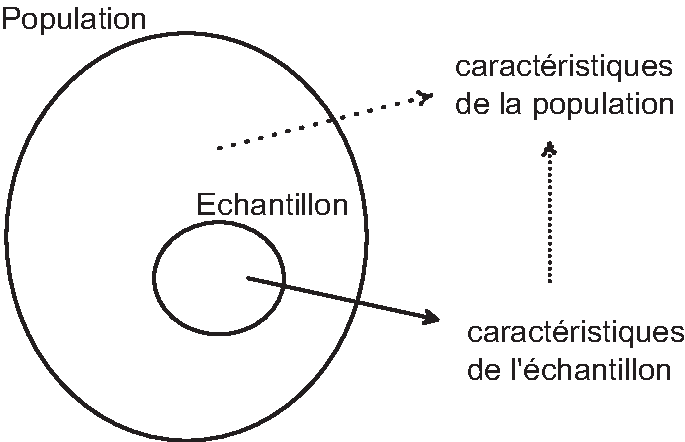
\includegraphics[scale=0.6]{inference}}
\caption{Principe de l'inf\'erence statistique}
\end{figure}

\begin{defi}
Un \emph{param\`etre} est une mesure calcul\'ee \`a partir d'une population enti\`ere.
\end{defi}

\begin{defi}
Une \emph{statistique} est une mesure calcul\'ee \`a partir d'un \'echantillon.
\end{defi}

Aussi longtemps que la population ne change pas, la valeur d'un param\`etre associ\'e \`a cette population ne varie pas. Par contre, la valeur d'une statistique d\'epend de l'\'echantillon s\'electionn\'e. Il existe donc g\'en\'eralement une diff\'erence entre la valeur d'un param\`etre, et son estimation par une statistique.

\begin{defi}
L'\emph{erreur d'\'echantillonnage} est la valeur de la diff\'erence entre une statistique et le param\`etre \'evalu\'e.
\end{defi}


% La statistique inf\'erentielle a les objectifs suivants:
% \begin{itemize}
% \item D\'eterminer des lois g\'en\'erales \`a partir d'un \'echantillon de donn\'ees.
% \item Estimer un param\`etre.
% \item Tester une hypoth\`ese.
% \item Evaluer la fiabilit\'e des r\'esultats.
% \end{itemize}

\chapter{Distributions continues}

Les donn\'ees peuvent provenir d'\'ev\'enements ponctuels comme le nombre de personnes entrant dans une banque en 1 heure, ou le nombre d'appels t\'el\'ephonique \`a faire afin de trouver 10 acheteurs d'un nouveau produit. Mais souvent, les donn\'ees sont continues, comme la quantit\'e de panure sur les mets \`a base de poisson, la longueur de coupes d'aciers, le temps de recharge d'une batterie de t\'el\'ephone, $\ldots$ .

Afin de mod\'eliser ces ph\'enom\`enes de type continu, nous utilisons des distributions continues, comme
\begin{itemize}
	\item la loi uniforme
	\item la loi normale
	\item la loi exponentielle
	\item ....
\end{itemize}

Des \emph{tables statistiques} sont disponibles pour chacune de ces lois, ainsi que des fonctions associ\'ees dans les logiciels de bureautique (MS Excel, Calc d'Openoffice, Gnumeric, ...) ou sp\'ecialis\'es (R).

\subsubsection{Variable al\'eatoire continue}
Une variable al\'eatoire continue $X$ prend ses valeurs dans un intervalle qui est un sous-ensemble de l'ensemble des r\'eels $\IR$ :
$$X \in [u,v]$$
avec $u,v\in\IR, u < v$

Le nombre de valeurs possibles de $X$ \'etant infini, chacune de ces valeurs a une probabilit\'e nulle. En revanche, il est possible de calculer la probabilit\'e associ\'ee \`a n'importe quel sous-intervalle $[a, b]$ de $[v,w]$ :
$$\begin{array}{ll}
	P(X = x) = 0 & \forall x \in [v,w]\\
  P(X \in [a, b]) \geq 0 & \forall a < b, [a, b] \subseteq [v,w]$$
\end{array}$$

\subsubsection{Fonction de densit\'e}
Une distribution continue est d\'efinie soit par sa fonction de densit\'e, soit par sa fonction de r\'epartition.

Une distribution continue peut \'etre repr\'esent\'ee par un histogramme. Si l'on dispose d'un grand nombre d'observations, il est possible de d\'efinir des classes de tr\`es petites amplitudes. A la limite, les classes deviennent d'amplitude nulle et l'histogramme devient une courbe. Cette courbe est la fonction de densit\'e de la variable al\'eatoire continue X, not\'ee $f(x)$.

La fonction de densit\'e n'est pas une distribution de probabilit\'e. En effet, pour tout $x$ appartenant \`a l'intervalle $[v,w]$, $P(X = x) = 0$, mais $f(x) \geq 0$.

En revanche, l'aire sous la courbe d'une fonction de densit\'e doit valoir 1, qui est la somme de toutes les probabilit\'es. Ainsi, la relation suivante est v\'erifi\'ee pour toute fonction de densit\'e
$$P(X \in ] -\infty,\infty[) = 1$$

\subsubsection{Fonction de r\'epartition}
La probabilit\'e d'\'etre dans un intervalle de longueur $dx$ tr\`es petit est donn\'ee par $f(x) dx$ :
$$P(X \in [x, x + dx]) = f(x) dx$$

La probabilit\'e de se trouver dans un intervalle $[a, b]$ est d\'efinie comme l'aire sous la fonction de densit\'e.
Math\'ematiquement, cela revient \`a calculer l'int\'egrale de la fonction $f(x)$ entre $a$ et $b$ :
$$P(X \in [a, b]) = \int^b_a f(x) dx$$

\begin{defi}
La fonction de r\'epartition, not\'ee $F(a)$, exprime pour une variable al\'eatoire $X$ la probabilit\'e d'\'etre inf\'erieure ou \'egale \`a $x$. Cela correspond \`a la surface sous la fonction de densit\'e \`a gauche de $x$ :

$$F(a) = P(X \leq a) = \int^a_{-\infty} f(x) dx$$
\end{defi}

\begin{pro}
La fonction de r\'epartition est telle que
\begin{itemize}
	\item $F(-\infty) = 0$, 
	\item $F(\infty) = 1$
	\item $P(X <a) = P(X \leq a) = F(a)$
  \item $P(X \in [a, b]) = F(b) - F(a)$
  \item Par compl\'ementarit\'e, $P(X>a) = 1- P(X\leq a) = 1-F(a)$
\end{itemize}
\end{pro}

\subsubsection{Esp\'erance et variance}

\begin{defi}
L'\emph{esp\'erance math\'ematique} d'une variable al\'eatoire continue $X$ le nombre
$$\E(X)=\int^{\infty}_{-\infty} x f(x) dx$$
\end{defi}

\begin{defi}
La \emph{variance} d'une variable al\'eatoire continue $X$ le nombre
$$\var(X)=\E\left[ X-\E(X)\right]^2 = \E(X^2)-\left[ \E(X)\right]^2$$
\end{defi}

\section{Loi normale}
La loi la plus utilis\'ee pour d\'ecrire des ph\'enom\`enes par une variable al\'eatoire continue est la loi normale. Par exemple, la description du poids, de la taille, du remplissage de r\'ecipients, ... Cette loi est abondamment utilis\'ee lors de l'inf\'erence statistique.

La repr\'esentation graphique de la loi normale est une courbe en forme de cloche, sym\'etrique.
$$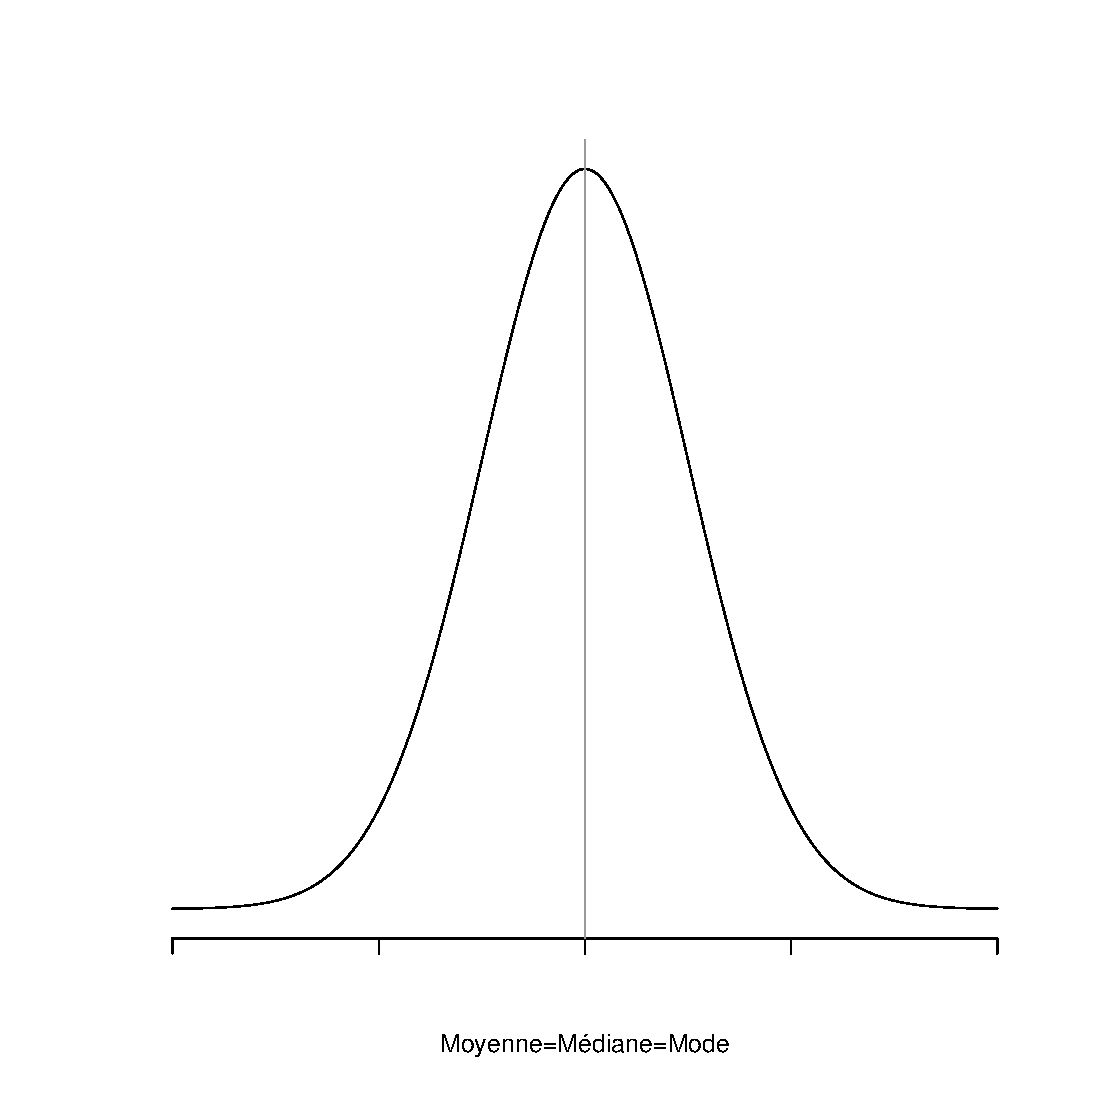
\includegraphics[scale=0.5]{norm_0_1}$$

\begin{defi}
La \emph{densit\'e de probabilit\'e normale} s'exprime par
$$f(x)=\frac{1}{\sigma\sqrt{2\pi}}e^{-\frac{(x-\mu)^2}{2\sigma^2}}$$
o� $\mu$ est la moyenne et $\sigma$ est l'\'ecart type
\end{defi}

La loi normale, not\'ee $\mathcal{N}(\mu,\sigma^2)$, comporte deux param\`etres $\mu$ et $\sigma^2$, qui d\'eterminent la position et la forme de la distribution. Il existe donc une famille de lois normales, et non pas une seule, qui se diff\'erencient par leur moyenne et leur \'ecart type.

\begin{pro}
\begin{itemize}
	\item Le point le plus \'elev\'e de la courbe normale correspond \`a la moyenne, qui est aussi la m\'ediane et le mode de la distribution.
  \item La distribution normale \'etant sym\'etrique, son  coefficient d'asym\'etrie (skewness) est nul.
  \item L'\'ecart type d\'etermine la largeur de la courbe. Plus sa valeur est \'elev\'ee, plus la courbe sera large et aplatie.
	\item La variable al\'eatoire associ\'ee peut prendre n'importe quelle valeur r\'eelle dans $]-\infty, \infty [$.
\end{itemize}
\end{pro}

La probabilit\'e est repr\'esent\'ee par l'aire sous la courbe de densit\'e $f(x)$. L'aire totale vaut 1 car il s'agit d'une probabilit\'e. Comme la loi normale est sym\'etrique, la probabilit\'e $P(X\leq\mu)=P(X\geq\mu)=0.5$, et par cons\'equent
$$P(X\leq x) = 1-P(X\geq x)$$
$$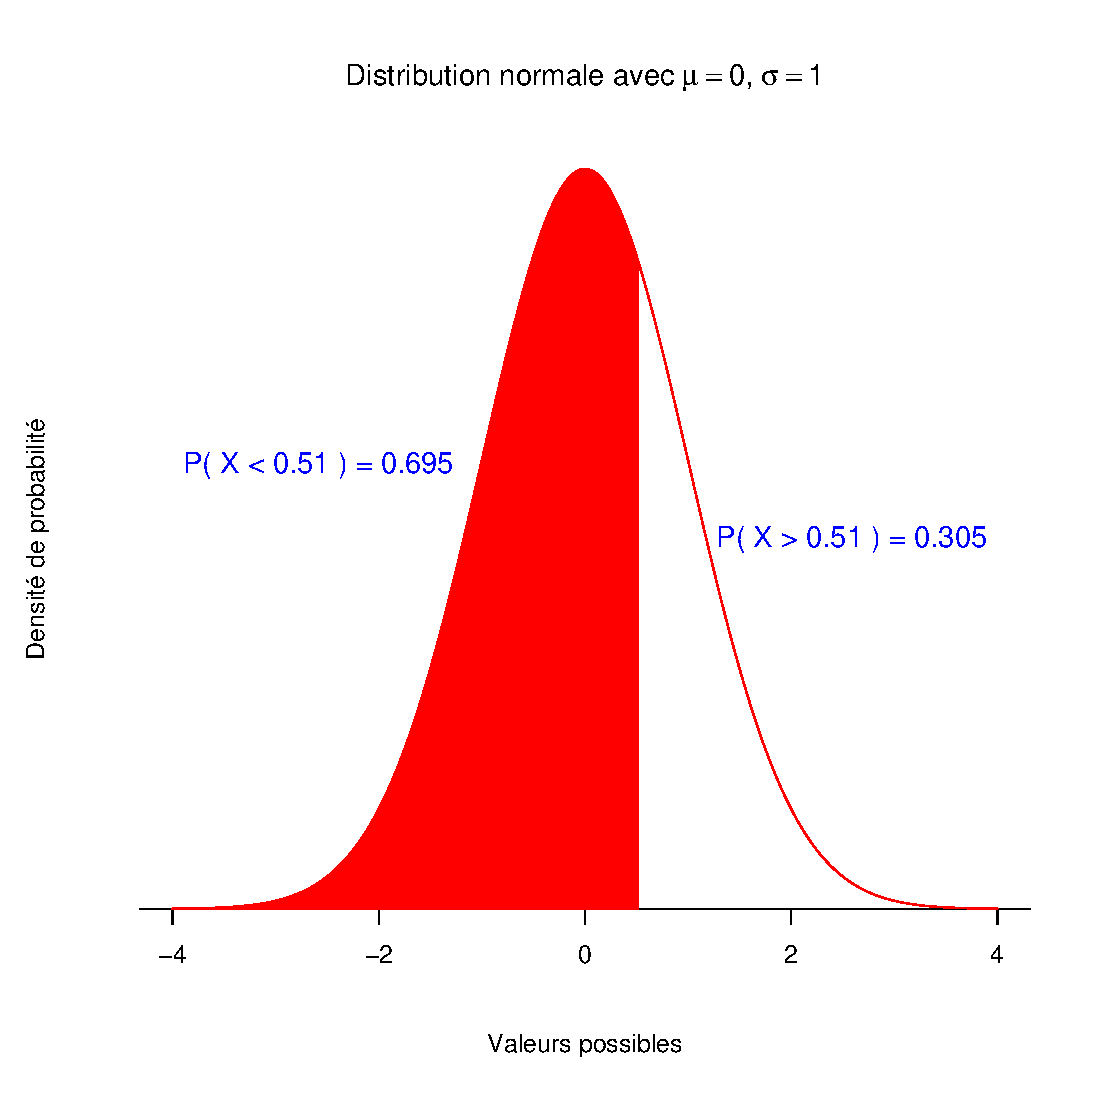
\includegraphics[scale=0.5]{norm_table}$$

En variant les param\`etres $\mu$ et $\sigma^2$ de la loi normale, nous obtenons diff\'erentes lois normales. Ainsi, il n'existe pas une seule loi normale, mais une multitudes de loi normales qui se diff\'erentient par leurs param\`etres.

$$
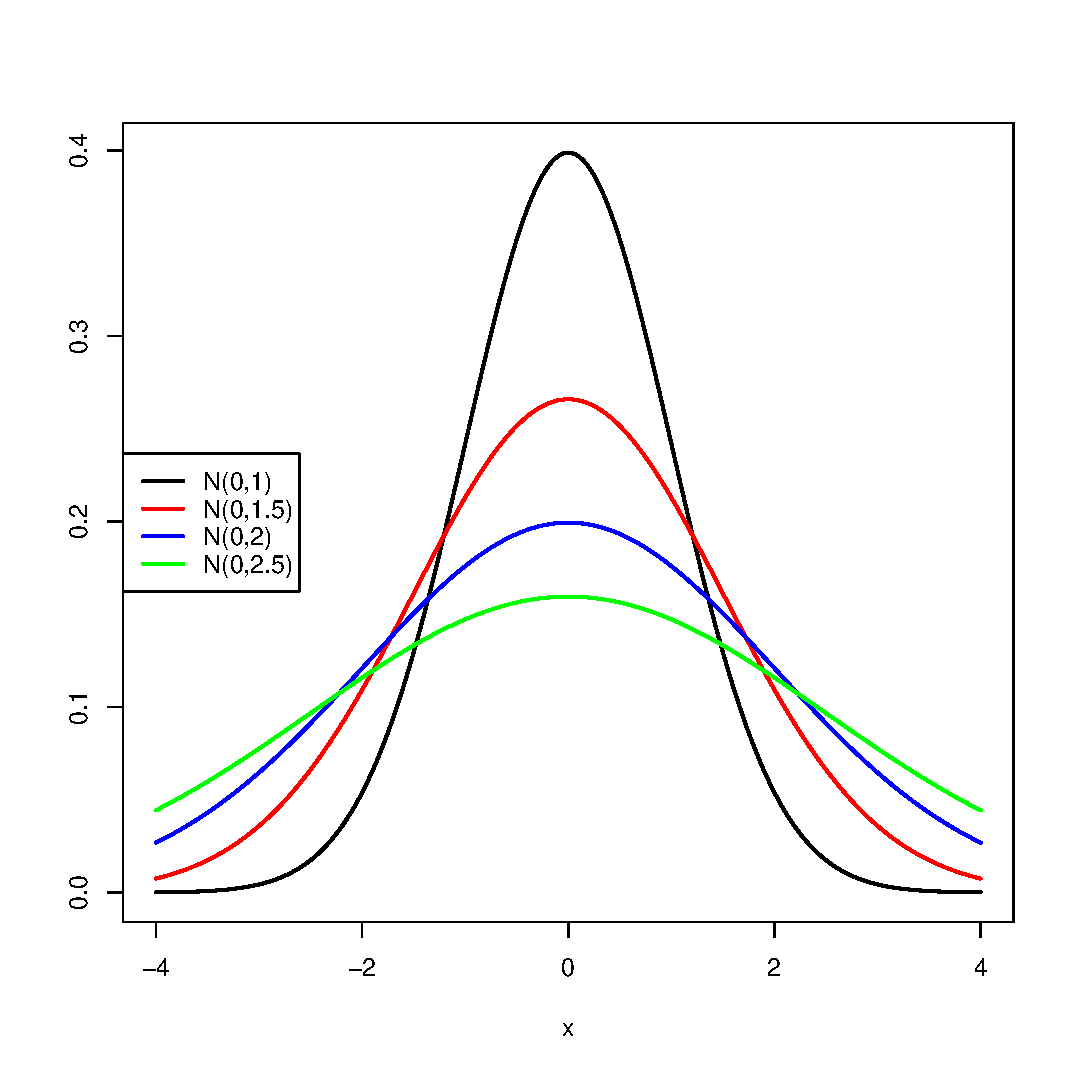
\includegraphics[scale=0.4]{normalesMu0}
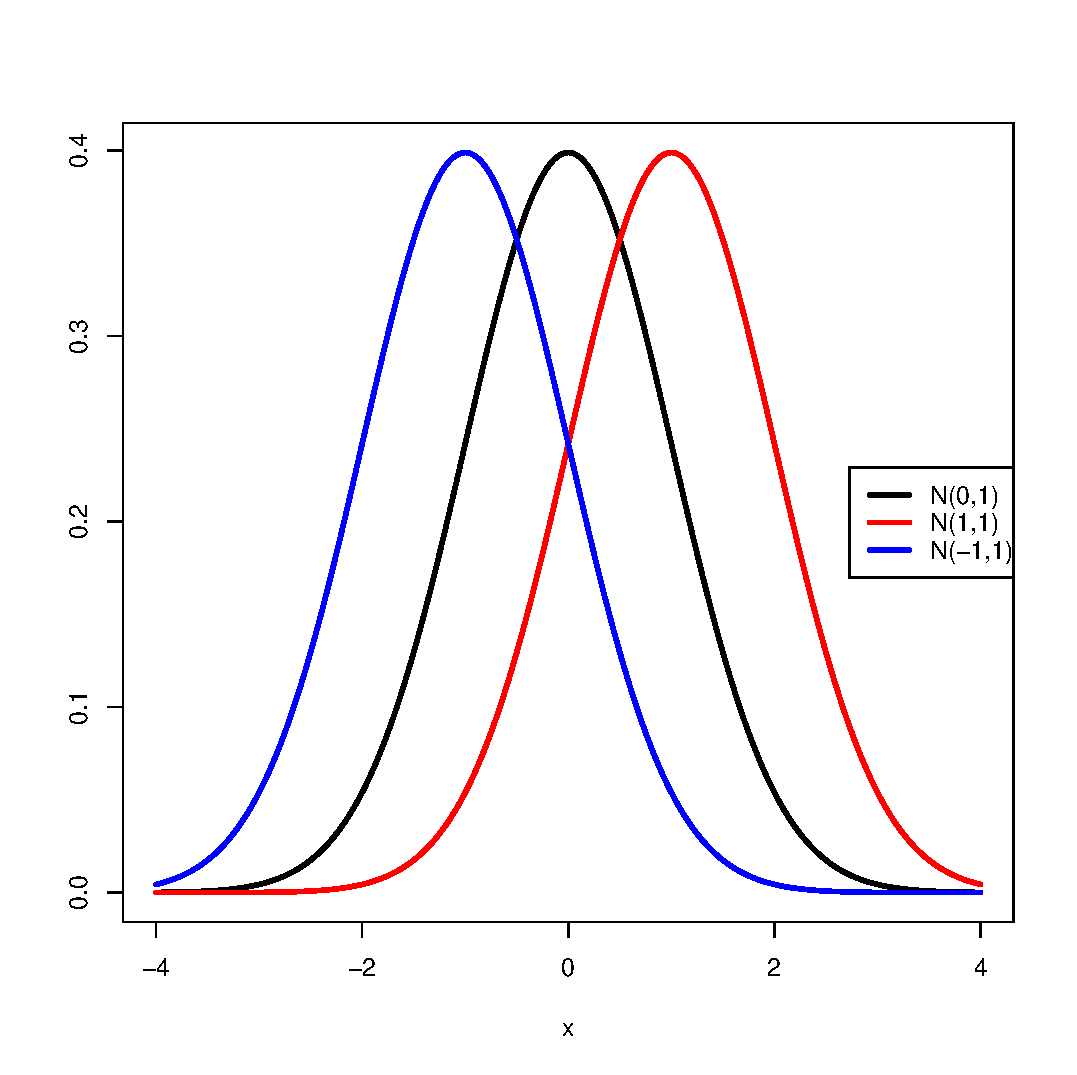
\includegraphics[scale=0.4]{normalesV1}$$

Il existe une distribution normale de r\'ef\'erence, de moyenne 0 et de variance 1, dite aussi distribution $Z$.

\begin{defi}
Une loi normale de moyenne nulle et d'\'ecart type 1 est dite \emph{loi normale centr\'ee r\'eduite}, aussi dite \emph{loi normale standard}. La fonction de densit\'e est alors
$$f(x)=\frac{1}{\sqrt{2\pi}}e^{-\frac{x^2}{2}}$$
\end{defi}

La lettre $Z$ est habituellement utilis\'ee pour d\'esigner la variable al\'eatoire continue dont la loi est normale centr\'ee r\'eduite. Il est toujours possible de transformer une variable al\'eatoire $X$ distribu\'ee selon une loi normale $\mathcal{N}(\mu,\sigma^2)$, en une variable $Z$ distribu\'ee selon une loi normale centr\'ee r\'eduite $\mathcal{N}(0,1)$. La transformation consiste \`a soustraire de $X$ la moyenne $\mu$, puis de diviser par l'\'ecart type $\sigma$
$$X\sim \mathcal{N}(\mu,\sigma^2)\quad\Rightarrow\quad Z=\frac{X-\mu}{\sigma}\sim\mathcal{N}(0,1)$$
Les probabilit\'es suivantes sont alors \'equivalentes, avec $X\sim\mathcal{N}(\mu,\sigma^2)$

$$X\leq x\quad\Rightarrow\quad Z\leq\frac{x-\mu}{\sigma}$$
$$P(X\leq x)=P(Z\leq\frac{x-\mu}{\sigma})$$

\begin{ex}
Si $X$ est une variable al\'eatoire suivant une loi normale de centre $\mu=100$ et d'\'ecart type $\sigma=50$, i.e. 
$$X\sim\norm (100,2500)$$ 
alors la $z$ valeur associ\'ee est 
$$Z=\frac{X-\mu}{\sigma}\sim\norm (0,1)$$
\vspace{5mm}

%$$
%	% \usepackage{pst-plot}
%\begin{pspicture}(-0.5,-1)(2.5,2.1)
%\psset{linewidth=0.5pt,xunit=3cm,yunit=3cm}
%\parametricplot[plotpoints=100]{-0.5}{2.5}{t 1 0.5 2 3.1416 mul sqrt mul div 2.71828 t 1 sub 2 exp 2 0.5 2 exp mul div neg exp mul}
%\psaxes[arrowscale=1.5,ticks=none,labels=none]{->}(-0.5,0)(2.5,1.0)
%\psline(1,-0.1)(1,0.1)
%\uput[90](1.0,-0.3){100}
%\uput[90](1.0,-0.45){\red 0}
%\psline(2.0,-0.1)(2.0,0.1)
%\uput[90](2.0,-0.3){200}
%\uput[90](2.5,-0.3){X}
%\uput[90](2.0,-0.45){\red 2}
%\uput[90](2.5,-0.45){\red Z}
%\uput[90](2,0.8){$X\sim\norm (100,2500)$}
%\uput[90](2,0.5){\red $Z\sim\norm (0,1)$}
%\end{pspicture}$$

%\newcommand{\sigma}{50}
%\newcommand{\moyenne}{100}
%% temporary off because of a bug of tikz
%\shorthandoff{:}
%$$
%\begin{tikzpicture}[scale=0.8, domain=0:4]
%\draw[->] (-0.2,0) -- (4.2,0);
%\draw[->] (0,-0.2) -- (0,4);
%%\draw plot (\x,{1/{\sigma*sqrt(2*pi)}*exp(-pow(\x-\moyenne,2)/{2*pow(\sigma,2)})}) ;
%\foreach \pos/\label in {1/100,2/200,3/300,4/X}
%        \draw (\pos,0) -- (\pos,-0.1) (\pos cm,-3ex) node
%            [anchor=base,fill=white,inner sep=1pt]  {\label};
%\foreach \pos/\label in {1/0,2/2,3/4,4/Z}
%        \draw [color=red] (\pos cm,-6ex) node
%            [anchor=base,fill=white,inner sep=1pt]  {\label};
%\node [right] at (2,3) {$X\sim\norm (100,2500)$};
%\node [right, color=red] at (2,2.3) {$Z\sim\norm (0,1)$};
%\end{tikzpicture}
%$$
%\shorthandon{:}

$$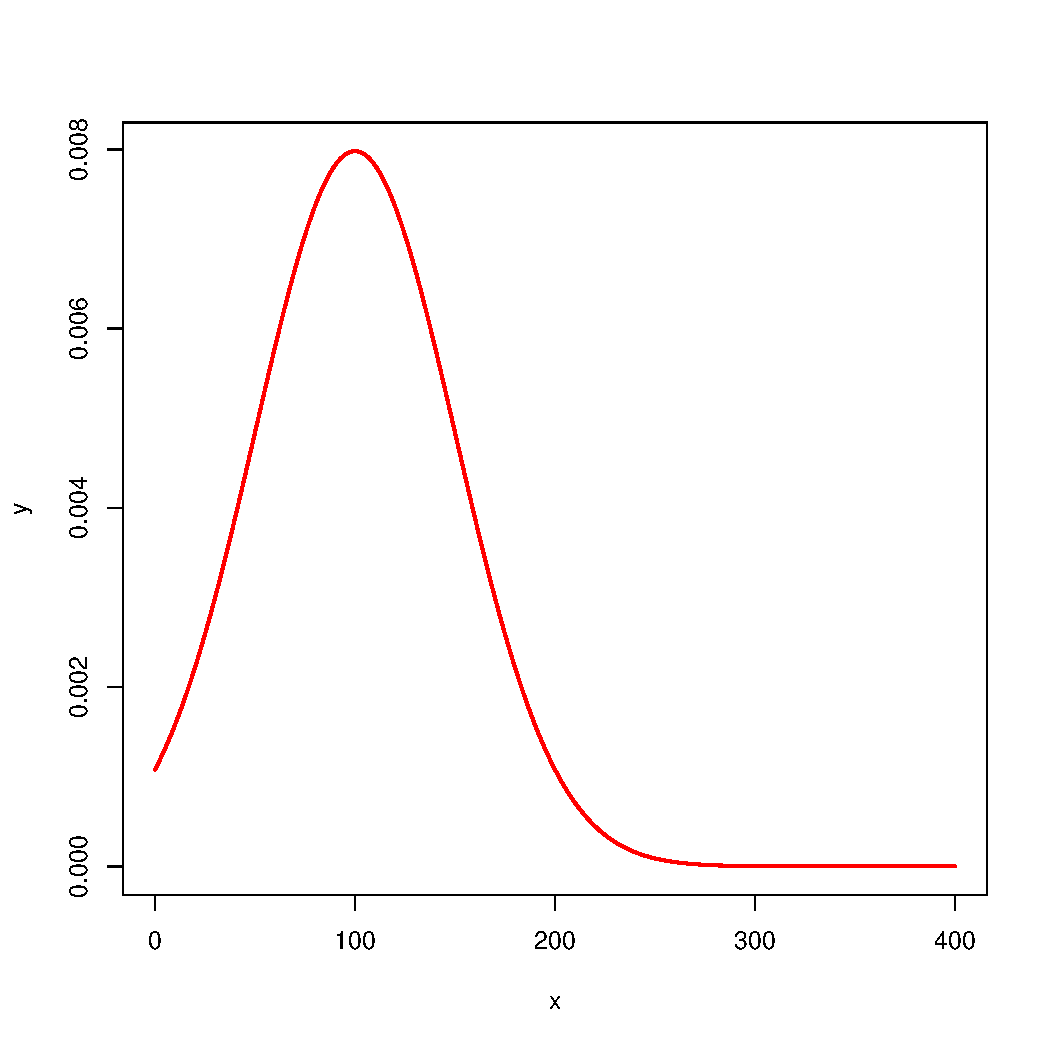
\includegraphics[scale=0.4]{Rnormal.pdf}$$

Ainsi, si $X=200$, alors $Z=\frac{200-100}{50}=2$. Cela signifie que $X=200$ est \'eloign\'e de 2 \'ecarts type au del\`a de la moyenne.\\
Nous avons alors $100+2*50 = 200 = X$
\end{ex}

\paragraph{Table de la loi normale}
La table de la loi normale donne les probabilit\'es d'occurrence jusqu'\`a la z-valeur consid\'er\'ee. La ligne donne la valeur de z jusqu'au dixi\`eme, et la colonne donne la valeur de z au centi\`eme.

\begin{ex}
\begin{itemize}
	\item La z-valeur associ\'ee \`a la ligne 0.5 et \`a la colonne 0.01 correspond \`a Z=0.51.\\
L'intersection de la ligne et de la colonne donne la probabilit\'e cherch\'ee:\\
$P(Z\leq 0.51)=0.6950$
  \item $P(Z\geq 0.51)=1-0.6950 = 0.305$ par compl\'ementarit\'e.
  \item $P(Z\leq -0.51) = P(Z\geq 0.51) = 0.305$ par sym\'etrie.
\end{itemize}
\end{ex}

\paragraph{R\`egle empirique}
En pratique, de nombreux ensembles de donn\'ees ont une distribution en forme de cloche. Dans ce cas, on peut utiliser une r\`egle empirique, fond\'ee sur une distribution de probabilit\'e normale:
\begin{itemize}
\item Environ 68\% des observations se situent dans l'intervalle $[\bar{x}-s;\bar{x}+s]$
\item Environ 95\% des observations se situent dans l'intervalle $[\bar{x}-2s;\bar{x}+2s]$
\item Environ 99.7\%  des observations (presque toutes) se situent dans l'intervalle\\ $[\bar{x}-3s;\bar{x}+3s]$
\end{itemize}

\vspace{5mm}
Les variables centr\'ees r\'eduites $Z$ permettent de d\'etecter des valeurs singuli\`eres de la mani\`ere suivante:
si les donn\'ees semblent \'etre le r\'esultat d'une variable al\'eatoire suivant une loi normale, presque toutes les observations devraient se trouver entre la moyenne et $\pm$ 3 \'ecarts type. Il est alors recommand\'e de consid\'erer toute observation dont la valeur de $Z$ se situe en dehors de cet intervalle comme \'etant singuli\`ere.

\section{Loi de Student ($\st_n$)}

William Gosset, alors qu'il travaillait pour la brasserie Guinness \`a Dublin, avait l'interdiction de publier le r\'esultat de ses travaux. Apr\`es avoir suivi un cours de Statistiques donn\'e par Karl Pearson, il prit le pseudonyme de ''Student'' pour publier la distribution du m�me nom en 1908.

\subsection{Loi de Student \`a $n$ degr\'es de libert\'e}

La distribution de Student, aussi appel\'ee $t$-distribution,  est une famille de distribution en forme de cloche et sym\'etrique. Elle est similaire \`a la distribution normale, mais avec des valeurs plus grandes aux extr\'emit\'es ($x$ petit ou $x$ grand). Elle se caract\'erise par le nombre de degr\'es de libert\'e.

\begin{center}
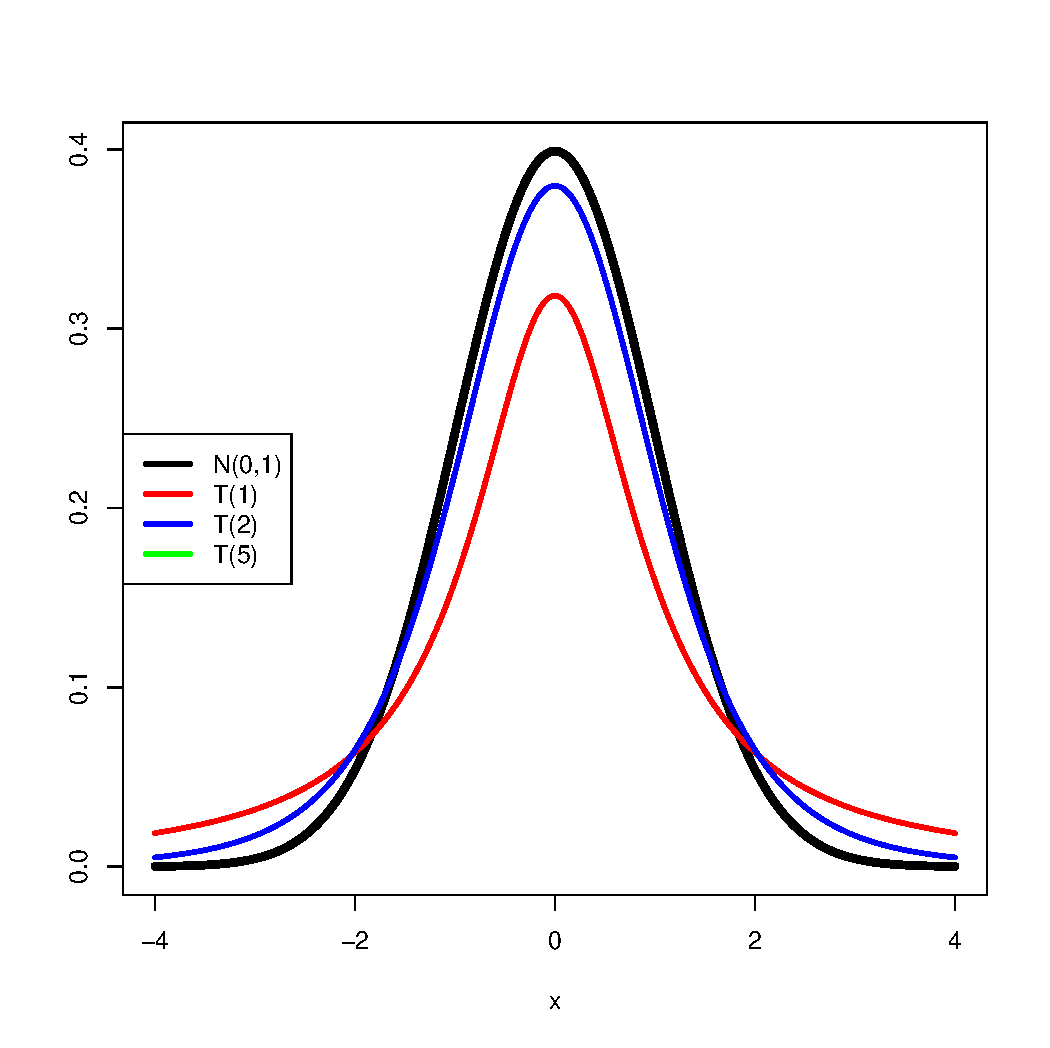
\includegraphics[scale=0.7]{normalevsStudent}
\end{center}

Lorsque le nombre de degr\'es de libert\'e $n$ tend vers l'infini, la loi de Student tend vers la loi normale $\norm(0,1)$.

%Soit $Z$ et $Q_n$, deux variables al\'eatoires ind\'ependantes telles que
%$$Z \sim N(0,1)\quad\quad Q_n\sim\chi^2_n$$
%
%Alors,
%$$T_n = \frac{Z}{\sqrt{\frac{Q_n}{n}}} \sim St_n$$
\newpage
\begin{pro}
$\st_n$: loi de Student \`a $n$ degr\'es de libert\'e
\begin{itemize}
	\item $\E(\st_n) = 0\, , \quad n>1$\\
	L'esp\'erance tend vers l'infini lorsque $n=1$. On dit alors qu'elle n'existe pas.
	\item $\var (\st_n) =  \frac{n}{n-2} \, , \quad n>2$\\
	La loi de Student a une variance infinie pour $n\leq 2$
	\item La loi de Student est sym\'etrique autour de 0.
\end{itemize}
\end{pro}

On utilisera le th\'eor\`eme suivant qui permet de faire de l'inf\'erence sur la moyenne d'une loi normale
de moyenne $\mu$ inconnue et de variance $\sigma^2$ inconnue.:
\begin{theo}
Soit un \'echantillon al\'eatoire de taille $n$, de moyenne $\bar{x}$ et de variance $s^2$, issu d'une loi normale $\norm(\mu,\sigma^2)$. Alors
$$\frac{\bar{x}- \mu}{\frac{s}{\sqrt{n}}}\sim \st_{n - 1}$$
\end{theo}

\subsection{Table de Student}
La table de la loi de Student se lit pour l'essentiel comme la table de la loi du $\chi^2$. Chaque ligne correspond \`a un nombre de degr\'es de libert\'e $n$ et chaque colonne \`a une erreur de premi\`ere esp\`ece $\alpha$. L'intersection d'une ligne et d'une colonne donne le seuil $t_{\alpha,n}$ tel que
$$P(\st_n\geq t_{\alpha,n})=\alpha$$
La relation entre $p$ et $\alpha$ est $p=1-\alpha$.

\begin{ex}
$$P(\st_{10}\leq t_{\alpha,10}) = 0.95  \quad \Longrightarrow t_{0.05,10} = 1.8125$$
\end{ex}

\'etant donn\'e que la loi de Student est sym\'etrique autour de 0, seules les erreurs de premi\`ere esp\`ece $\alpha$ inf\'erieures \`a 0.5 sont donn\'ees. Les $\alpha > 0.5$ peuvent �tre retrouv\'ees, comme pour la loi normale, par sym\'etrie et compl\'ementarit\'e.





\section{Loi du chi carr� ($\chi^2$)}

\subsection{Loi du chi-2 � $n$ degr�s de libert�}
\begin{defi}
Soit $n$ variables al�atoires normales centr�es-r�duites $Z_i$, ind�pendantes les unes des autres et identiquement distribu�es: $Z_i  \mbox{ i.i.d.} \sim\norm(0,1)$, $i=1,2,\ldots,n$. Alors la variable form�e de la somme des carr�s de ces variables
$$Q_n = \sum_{i=1}^{n} Z_i^2 \sim \chi^2$$
suit une \emph{loi du $\chi^2$ � $n$ degr�s de libert�}.
\end{defi}

On note parfois $\chi^2(n)$ ou $\chi^2_n$ pour indiquer une loi du $\chi^2$ � $n$ degr�s de libert�

\begin{pro} La loi du $\chi^2$ � $n$ degr�s de libert� poss�de les propri�t�s suivantes
\begin{itemize}
	\item Son esp�rance vaut $n$
	%$\E (Q_n) = \sum_i\var (Z_i) = n$
	\item Sa variance vaut $2n$
	%$\var (Q_n)= \sum_i\var (Z_i^2) = 2n$
\end{itemize}
\end{pro}

%\begin{proof}
%$\chi^2=\frac{(n-1)s^2}{\sigma^2}=\frac{(n-1)\frac{\sum(x-\bar{x})^2}{n-1}}{\sigma^2}
%=\frac{\sum(x-\bar{x})^2}{\sigma^2} = \sum(\frac{x-\bar{x}}{\sigma})^2$
%\end{proof}
 
$$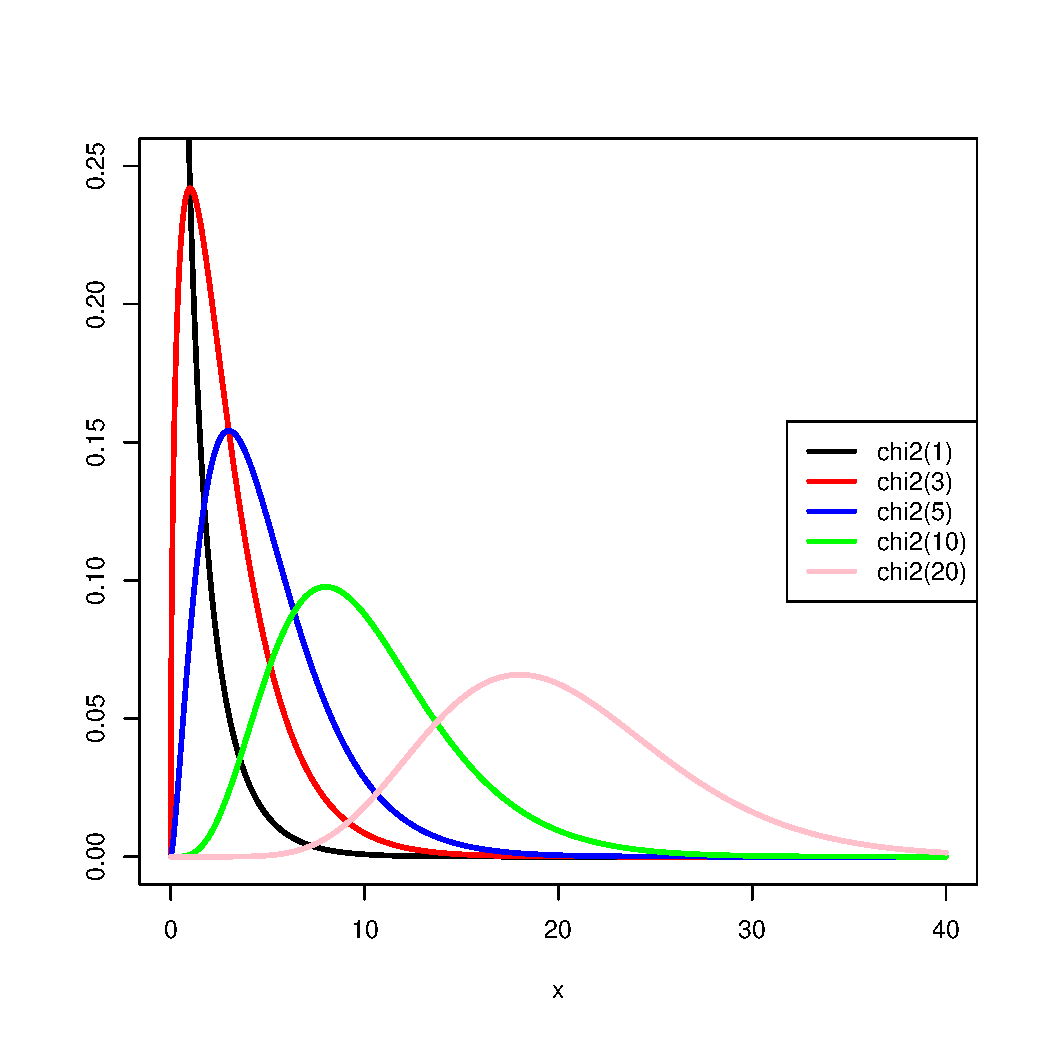
\includegraphics[scale=0.7]{chisquare}$$

\begin{rem}
La loi du chi-2 �tant d�finie comme une somme de carr�s, elle ne prend que des valeurs positives.
\end{rem}

Nous utiliserons la propri�t� suivante lorsque nous calculerons (cf. \ref{section:variance-estimation}
) un intervalle de confiance pour la variance d'une population.

\begin{pro}\label{pro:chi2}
La statistique $\chi^2$ � $n-1$ degr�s de libert� vaut
$$\chi^2 = \frac{(n-1)s^2}{\sigma^2}$$
o�\\
\begin{tabular}{ccl}
$\chi^2$ & = & variable chi-2 standard\\
$s^2$ &= &  variance de l'�chantillon\\
$\sigma^2$ & = & variance de la population\\
$n$ &= &  taille de l'�chantillon
\end{tabular}
\end{pro}


\subsection{Table du $\chi^2$}
\centerline{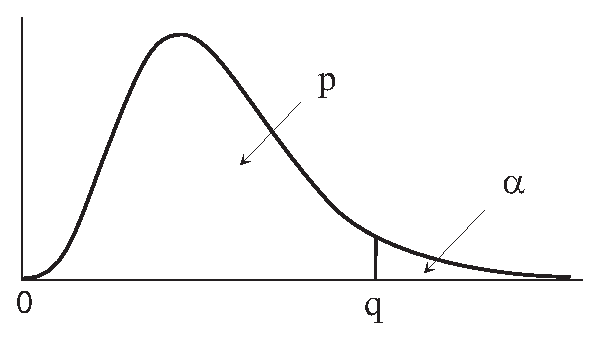
\includegraphics[width=10cm]{chi2b}}

Pour une variable $Q_n$ suivant une loi du $\chi^2$ � $n$ degr�s de libert�, $p = P(Q_n\leq q_{\alpha,n})$ et $\alpha = P(Q_n>q_{\alpha,n})$.
La relation entre $p$ et $\alpha$ est donn�e par 
$$p=1-\alpha$$

La table du $\chi^2$ en annexe \ref{sec:tablechideux} donne le seuil $q$ associ� � une erreur de premi�re esp�ce $\alpha$ (colonne) et un nombre de degr�s de libert� $n$ (ligne).

\begin{ex}
$P(Q_7 \leq q_{\alpha,7}) = 0.95$\\
Alors $\alpha=1-0.95=0.05$\\
Et donc $\quad q_{0.05,7} = 14.0671$
\end{ex}

%\section{Loi de Fisher-Snedecor}

\subsection{Loi de Fisher-Snedecor � $n$ et $m$ degr�s de libert�}
\begin{defi}
Soit $Q_n$ et $Q_m$ deux variables al�atoires ind�pendantes telles que
\begin{eqnarray*}
    Q_n & \sim & \chi^2_n\\
    Q_m & \sim & \chi^2_m
\end{eqnarray*}
Alors,
$$Y_{n,m} = \frac{\;\;\frac{Q_n}{n}\;\;}{\frac{Q_m}{m}} \sim F_{n,m}$$
$F_{n,m}$ est appel�e \emph{loi $F$ de Fisher-Snedecor} (ou plus simplement de Fisher) � $n$ et $m$ degr�s de libert�.
\end{defi}

\begin{rem}
La loi de Fisher �tant d�finie par le rapport de 2 quantit�s positives, elle ne prend donc que des valeurs positives.
\end{rem}

\begin{pro} La loi $F$ de Fisher poss�de les propri�t�s suivantes
\begin{itemize}
	\item $\E(Y_{n,m}) = \frac{m}{m-2}$, $m>2$\\
	L'esp�rance ne d�pend pas de $n$.\\
	\item $\var (Y_{n,m}) = \frac{2m^2(m+n-2)}{n(m-2)^2(m-4)}$, $m>4$
\end{itemize}
\end{pro}

\subsection{Table de Fisher}
Pour une probabilit� $p$ fix�e, la table de Fisher se lit en fonction des degr�s de libert� du num�rateur (colonne) et du d�nominateur (ligne). L'intersection de la ligne et de la colonne donne le seuil $f$ correspondant. Les tables les plus courantes sont celles correspondant � $p=95\%$ et $p=99\%$.
 
\begin{center}
\includegraphics[width=12cm]{Fisher}
\end{center}

\begin{eqnarray*}
p &=& P(Y_{n,m}\leq f)\\
\alpha &=& P(Y_{n,m}>f)
\end{eqnarray*}

\begin{ex}
$P(Y_{5,3}\leq f) = 0.95  \quad \Rightarrow \quad f=9.01$
$P(Y_{3,5}\leq f) = 0.95  \quad \Rightarrow \quad f=5.41$
\end{ex}
\chapter{Estimation}

L'estimation a pour objectif d'attribuer une valeur � un ou plusieurs param�tres de la population sur la base d'un �chantillon issu de celle-ci. L'estimation peut �tre ponctuelle ou par intervalle.


%%%%%%%%%%%%%%%%%%%%%%%%%%%%%%%%%%%%%%%%%%%%%%
%%                                          %%
%%     Estimation  ponctuelle               %%
%%                                          %%
%%%%%%%%%%%%%%%%%%%%%%%%%%%%%%%%%%%%%%%%%%%%%%
\section{Estimation ponctuelle}

\begin{defi}
Une \emph{estimation ponctuelle}, ou point d'estimation, est une valeur calcul�e � partir d'un �chantillon pour estimer un param�tre d'une population.
\end{defi}

\begin{ex}
Soit une variable al�atoire repr�sentant la taille des m�nages (nombre de personnes composant un m�nage) et soit deux
�chantillons al�atoires X et Y:

 \begin{center}
 \begin{tabular}{lcccccccc}
 �chantillon $X$ & $x_1$ & $x_2$ & $x_3$ & $x_4$ & $x_5$ & $x_6$ &
$x_7$ & $x_8$\\
 & 1 & 3 & 2 & 4 & 4 & 1 & 2 & 6\\
 \\
 �chantillon $Y$ & $y_1$ & $y_2$ & $y_3$ & $y_4$ & $y_5$\\
 & 2 & 2 & 1 & 1 & 3
 \end{tabular}
 \end{center}

\'Echantillon $X$: $\bar{x} = \frac{23}{8}$\\
\'Echantillon $Y$: $\bar{y} = \frac{9}{5}$\\
Les valeurs $\bar{x}$ et $\bar{y}$ sont des estimations ponctuelles de la taille moyenne des m�nage (=param�tre de la population).
\end{ex}

\subsection{Propri�t�s des estimateurs}

Chaque �chantillon conduit � une estimation diff�rente du param�tre. Il y a bien s�r des ensembles de valeurs qui sont plus ad�quates que d'autres pour un estimateur.

\begin{defi}
Une \emph{distribution d'�chantillonnage} est la distribution des valeurs possibles d'une statistique pour un �chantillon de taille fix�e, s�lectionn� � partir d'une population.
\end{defi}

%\begin{defi}
%La suite des valeurs possibles de l'estimateur $\hat\theta$ du param�tre $\theta$, ainsi que les probabilit�s correspondantes s'appelle la \emph{loi} de l'estimateur.
%\end{defi}

Ainsi, un estimateur $\hat{\Theta}$ est consid�r� comme une variable al�atoire dont le comportement en moyenne est
$$\E(\hat{\Theta})$$
et dont la variance est une mesure de dispersion des estimations
$$\var(\hat{\Theta})$$

Dans les situations o\`u l'esp�rance de l'estimateur est �gal au param�tre, on dit que l'estimateur est sans biais. Cependant, quel que soit le sondage (qui n'est pas un recensement), la diff�rence entre le point $\hat\theta$ calcul� et le param�tre $\theta$ de la population n'est pas connu. On attend d'un estimateur qu'il soit fiable, et aussi proche que possible de la v�ritable valeur du param�tre. Pour cela, deux propri�t�s sont souhaitables pour un estimateur $\hat{\Theta}$:

 \begin{itemize}
    \item l'absence de biais
    \item la convergence
 \end{itemize}

\begin{defi}
Le \emph{biais} est la quantit�
$$\E(\hat{\Theta}-\theta) = \E(\hat{\Theta})-\theta$$
Un estimateur est dit \emph{non-biais�} lorsque son esp�rance est
�gale � la vraie valeur du param�tre estim�:
$$\E(\hat{\Theta}) = \theta$$
\end{defi}

%------------------------------------
\begin{center}
 \begin{tabular}{ccc}
  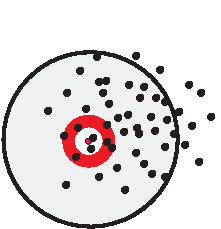
\includegraphics[width=5cm,clip]{cible_biais} & & 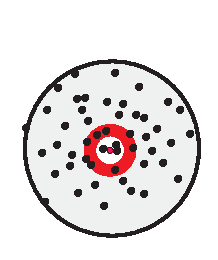
\includegraphics[width=4cm,clip]{cible_abs_biais}\\
  Biais & & Absence de bais	
 \end{tabular}
\end{center}
 %------------------------------------

\begin{defi}
 Un estimateur est dit \emph{convergent} si, lorsque la taille $n$ de l'�chantillon devient grande
\begin{enumerate}
	\item le biais dispara�t:
		$$\lim_{n\rightarrow\infty} \biais(\hat{\Theta}) = 0$$
  \item la variance devient nulle
  $$\lim_{n\rightarrow\infty} \var(\hat{\Theta}) = 0$$
\end{enumerate}
\end{defi}

Cela revient � dire que lorsque la taille de l'�chantillon augmente, l'estimation devient de plus en plus pr�cise.

\begin{defi}
Un estimateur sans biais et convergent est dit \emph{absolument correct}.
\end{defi}



\subsection{Estimation de la moyenne de la population}
Consid�rons un �chantillon de taille $n$.\\
La moyenne de la population, $\mu$, est estim�e � l'aide de la moyenne de l'�chantillon, not�e $\overline{x}$:
$$\hat{\mu} = \overline{x} = \frac{1}{n} \sum_{i=1}^n x_i$$

\begin{pro}
$\overline{x}$ est un estimateur absolument correct de la moyenne $\mu$.
\end{pro}

\begin{rem}
La moyenne tronqu�e, le mode et la m�diane calcul�s � partir d'un �chantillon sont aussi des estimateurs absolument
corrects pour respectivement la moyenne tronqu�e, le mode et la m�diane de la population.
\end{rem}




\subsection{Estimation de la variance de la population}
Consid�rons un �chantillon de taille $n$.\\
La variance de la population, $\sigma^2$, peut �tre estim�e � partir de la variance de  l'�chantillon. La premi�re id�e serait de prendre comme estimateur de $\sigma^2$
$$S^2 = \frac{1}{n} \sum_{i=1}^n (x_i-\overline{x})^2$$

Si nous calculons l'esp�rance de cet estimateur $S^2$ nous obtenons:\\
%$\begin{eqnarray*}
%    \E(S^2) & = & \var (x) - \var (\overline x)\\[1ex]
%        &=& \sigma^2 - \dfrac{\sigma^2}{n}\\[1ex]
%        & = & \boxed{\dfrac{(n-1)}{n}\,\sigma^2}
%\end{eqnarray*}$
$$\E(S^2)=\frac{(n-1)}{n}\,\sigma^2$$
$S^2$ est donc un estimateur biais� de $\sigma^2$

En revanche, on peut montrer que $S^2$ est un estimateur convergent de
$\sigma^2$
%$\biais (S^2) = -\,\dfrac{\sigma^2}{n}
%\xrightarrow[n\to\infty]{}0$\\[2ex]
%    $\var (S^2) = \tfrac{n-1}{n^2}\left(\tfrac{n-1}{n}\,\mu_4
%- \tfrac{n-3}{n}\,\sigma^4\right)
%\xrightarrow[n\to\infty]{}0$
%\textbf{$\Longrightarrow$ $S^2$ est un estimateur convergent de
%$\sigma^2$}\\

Ainsi, la variance de l'�chantillon, $S^2$, n'est pas un estimateur absolument correct de la variance de la population, car $S^2$ sous-estime la variance de la population.

Un meilleur estimateur $\hat{\sigma}^2$ de la variance de la population est obtenu en enlevant le biais de $S^2$:

%$$ \begin{eqnarray*}
%    \hat{\sigma}^2
%    &=& \frac{n}{n-1} \: S^2\\[2ex]
%    &=& \frac{1}{n-1} \sum_{i=1}^n (x_i-\overline{x})^2
% \end{eqnarray*}$$

$$ s^2 = \frac{1}{n-1} \sum_{i=1}^n (x_i-\overline{x})^2$$

\begin{pro}
% \begin{itemize}
%    \item $\E(\hat{\sigma}^2) = \sigma^2$ $\longrightarrow$ pas de
%biais\\
%    \item $\var (\hat{\sigma}^2) =
%\tfrac{1}{n-1}\left(\tfrac{n-1}{n}\,\mu_4 -
%\tfrac{n-3}{n}\,\sigma^4\right)
% \xrightarrow[n\to\infty]{} 0$
% \end{itemize}
$s^2$ est un estimateur absolument correct de la variance $\sigma^2$ de la population.
\end{pro}

Nous allons donc consid�rer dor�navant $s^2$ comme estimateur de la variance $\sigma^2$ d'une population. L'exemple suivant permet de constater que $s^2$ est un meilleur estimateur que $S^2$ de la variance r�elle $\sigma^2$.

%\begin{ex}
%Soit une variable al�atoire repr�sentant la taille des m�nages (nombre de personnes composant un m�nage) et soit deux
%�chantillons al�atoires X et Y:
%
% \begin{center}
% \begin{tabular}{lcccccccc}
% �chantillon $X$ & $x_1$ & $x_2$ & $x_3$ & $x_4$ & $x_5$ & $x_6$ &
%$x_7$ & $x_8$\\
% & 1 & 3 & 2 & 4 & 4 & 1 & 2 & 6\\
% \hline
% �chantillon $Y$ & $y_1$ & $y_2$ & $y_3$ & $y_4$ & $y_5$\\
% & 2 & 2 & 1 & 1 & 3\\
% \hline
% \end{tabular}
% \end{center}
%
% {\itshape Echantillon} $X$: $s_X^2$ = 2.61 $\longrightarrow$ $\hat{\sigma}^2$ = 2.98\\[1ex]{\itshape Echantillon} $Y$: $s_Y^2$ = 0.56
%$\longrightarrow$ $\hat{\sigma}^2$ = 0.7
%\end{ex}

\begin{ex}
% Prob et stat, Freddy Taillard p.14, exemple 3
Supposons que la population est compos�e des trois nombres 1,2 et 6.\\
La moyenne vaut
$$\mu =\frac{1+2+6}{3}=3$$
et la variance vaut
$$\sigma^2 = \frac{(1-3)^2+(2-3)^2+(6-3)^2}{3}=\frac{14}{3}$$
Formons tous les �chantillons possibles de taille 2 en pr�levant 2 �l�ments au hasard dans la population. Comme la population n'est pas tr�s vaste, on replace le premier �l�ment tir� dans la population avant de tirer le second. Nous obtenons les $\overline{A_3^2}=3^2=9$ �chantillons possibles suivants:
$$(1;1), (1;2), (1;6), (2;1), (2;2), (2;6), (6;1), (6;2), (6;6)$$
Les moyennes de ces couples de nombres sont:
$$1, \frac{3}{2}, \frac{7}{2}, \frac{3}{2}, 2, 4, \frac{7}{2}, 4, 6$$
Les variances $S^2$ de ces couples de nombres sont:
$$0, \frac{1}{4}, \frac{25}{4}, \frac{1}{4}, 0, 4, \frac{25}{4}, 4, 0$$
La moyenne des variances de ces couples de nombres est �gale � $\frac{7}{3}$, ce qui n'est pas �gale � la variance de la population ($\frac{14}{3}$).
En revanche,
$$\frac{n}{n-1}\cdot\frac{7}{3}=\frac{2}{2-1}\cdot\frac{7}{3}=\frac{14}{3}$$

Ainsi, afin d'obtenir une estimation non biais�e de la variance d'une population, on utilisera la formule
$$\hat{\sigma^2} = s^2=\frac{\sum\limits_{i=1}^n (x_i-\bar{x})^2}{n-1}$$
o� $n$ d�signe le nombre d'observations dans l'�chantillon
\end{ex}

\begin{rem}
Beaucoup de calculatrices et de logiciels statistiques donnent par d�faut $\hat{\sigma}^2$ plut�t que $S^2$. La valeur donn�e par $\hat{\sigma}^2$ est correcte lorsque l'on veut estimer un param�tre de la population. En revanche, lorsque l'on fait de la statistique descriptive sur les donn�es, c'est � dire lorsque les donn�es sont consid�r�e comme une population, il faut utiliser $S^2$. La relation entre $\hat{\sigma}^2$ et $S^2$ est la suivante:
$$ \hat{\sigma}^2 = \frac{n}{n-1}S^2$$
\end{rem}


%%%%%%%%%%%%%%%%%%%%%%%%%%%%%%%%%%%%%%%%%%%%%%
%%                                          %%
%%         Th�or�me central limite          %%
%%                                          %%
%%%%%%%%%%%%%%%%%%%%%%%%%%%%%%%%%%%%%%%%%%%%%%
\section{Th�or�me central limite}

L'�cart type $\sigma(\hat\Theta)$ et la variance $\var(\hat\Theta)$ sont des mesures de pr�cision de l'estimateur $\hat\Theta$. Plus ils sont grands, moins bonne est l'estimation du param�tre �tudi�. Afin d'am�liorer la pr�cision, il faut alors soit trouver une meilleure formule pour estimer le param�tre, soit changer la m�thode d'�chantillonnage. En pratique, on cherche le plus souvent � r�duire la variance en premier.


\subsection{Distribution de la moyenne d'un �chantillon}

Le th�or�me suivant indique que si la population suit une loi normale, alors l'�chantillon aussi.

\begin{theo}
Si une population est normalement distribu�e, de moyenne $\mu$ et d'�cart type $\sigma$, alors la distribution d'�chantillonnage de la moyenne $\bar{x}$ est aussi normalement distribu�e de m�me moyenne que la population
$$\mu_{\bar{x}}=\mu$$
et dont l'�cart type vaut l'�cart type de la population divis� par la racine carr�e de la taille de l'�chantillon
$$\sigma_{\bar{x}}=\frac{\sigma}{\sqrt{n}}$$
\end{theo}

\begin{defi}
L'�cart type de la distribution d'�chantillonnage de la moyenne, aussi appel�e \emph{erreur standard de la moyenne}, est le terme
$$\sigma_{\bar{x}}=\frac{\sigma}{\sqrt{n}}$$
\end{defi}

\begin{rem}
Notons que l'erreur standard de la moyenne est toujours inf�rieure ou �gale � l'�cart type de la population.
\end{rem}

La distribution d'�chantillonnage de la moyenne est compos�e de toutes les moyennes possibles sur tous les �chantillons de m�me taille. La distance relative d'une moyenne particuli�re � la moyenne d'�chantillonnage (i.e. l'esp�rance) peut �tre d�termin�e par une variable centr�e r�duite $z$. Cette variable $z$ mesure le nombre d'�cart type entre la moyenne (i.e. l'esp�rance) et une valeur particuli�re (i.e. une moyenne d'un �chantillon particulier).

\begin{defi}
La variable centr�e r�duite associ�e � la moyenne d'�chantillonnage est la variable
$$z=\frac{\bar{x}-\mu}{\frac{\sigma}{\sqrt{n}}}$$
\begin{tabular}{ccl}
	$\bar{x}$ & = & moyenne de l'�chantillon\\
	$\mu$ & = & moyenne de la population\\
	$\sigma$ & = & �cart type de la population\\
	$n$ & = & taille de l'�chantillon
\end{tabular}
\end{defi}


\begin{ex}
D'apr�s l'�tiquetage, la quantit� de poisson contenue dans un plat surgel� de 1 kg  suit une loi normale, de moyenne 500 g, avec une variation de $\pm 100$ grammes (�cart type). Un magazine de consommateurs ach�te 25 de ces plats surgel�s et v�rifie la quantit� de poisson. Les r�sultats du test donne une moyenne de 490 g par plat. Peut-on affirmer qu'il y a tromperie du consommateur?\\
\begin{enumerate}
	\item La moyenne pour cet �chantillon est de $\bar{x} = 490$
	\item La distribution d'�chantillonnage de la moyenne doit suivre une loi normale de moyenne $\mu_{\bar{x}}=\mu=500$ et d'�cart type $\sigma_{\bar{x}}=\frac{\sigma}{\sqrt{n}}=\frac{100}{\sqrt{25}}=20$
	\item L'�v�nement d'int�r�t est le suivant: Comme la moyenne d'�chantillon trouv�e (490) est inf�rieure � la moyenne attendue (500), nous d�sirons conna�tre la probabilit� d'un tel �v�nement
	$$P(\bar{x}\leq 490)=?$$
	\item Conversion de la moyenne d'�chantillonnage en une valeur centr�e r�duite
	 $$z=\frac{\bar{x}-\mu}{\frac{\sigma}{\sqrt{n}}}=\frac{490-500}{\frac{100}{\sqrt{25}}}=-0.5$$
	\item Utiliser la distribution normale centr�e r�duite pour d�terminer la probabilit� d�sir�e
	$$P(z\leq -0.5)=0.3085$$
\end{enumerate}
Il y a donc  une probabilit� d'environ 0.3 que la moyenne d'un �chantillon de 25 plats surgel� soit d'au plus 490 grammes.
\end{ex}

\begin{rem}
Si la taille de l'�chantillon est \emph{plus du 5\%} de la taille de la population, et que l'�chantillon tir� est fait \emph{sans remise}, alors un facteur de correction pour une population finie doit �tre consid�r�. Ce facteur de correction, qui s'applique � la valeur de l'�cart type $\sigma_{\bar{x}}$, est de
$$\sqrt{\frac{N-n}{N-1}}$$
o�\\
$N$ = taille de la population\\
$n$ = taille de l'�chantillon
\end{rem}

Beaucoup de m�thodes statistiques reposent sur l'hypoth�se selon laquelle les donn�es observ�es sont distribu�es selon une loi normale. En pratique, cela n'est pas toujours v�rifi�, mais le {\bfseries th�or�me central limite} assure que m�me si la population ne satisfait pas � la normalit�, la moyenne d'un �chantillon de grande taille issu de celle-ci est distribu�e de fa�on normale, ce qui est suffisant pour l'emploi de la plupart des outils statistiques.

\begin{figure}
  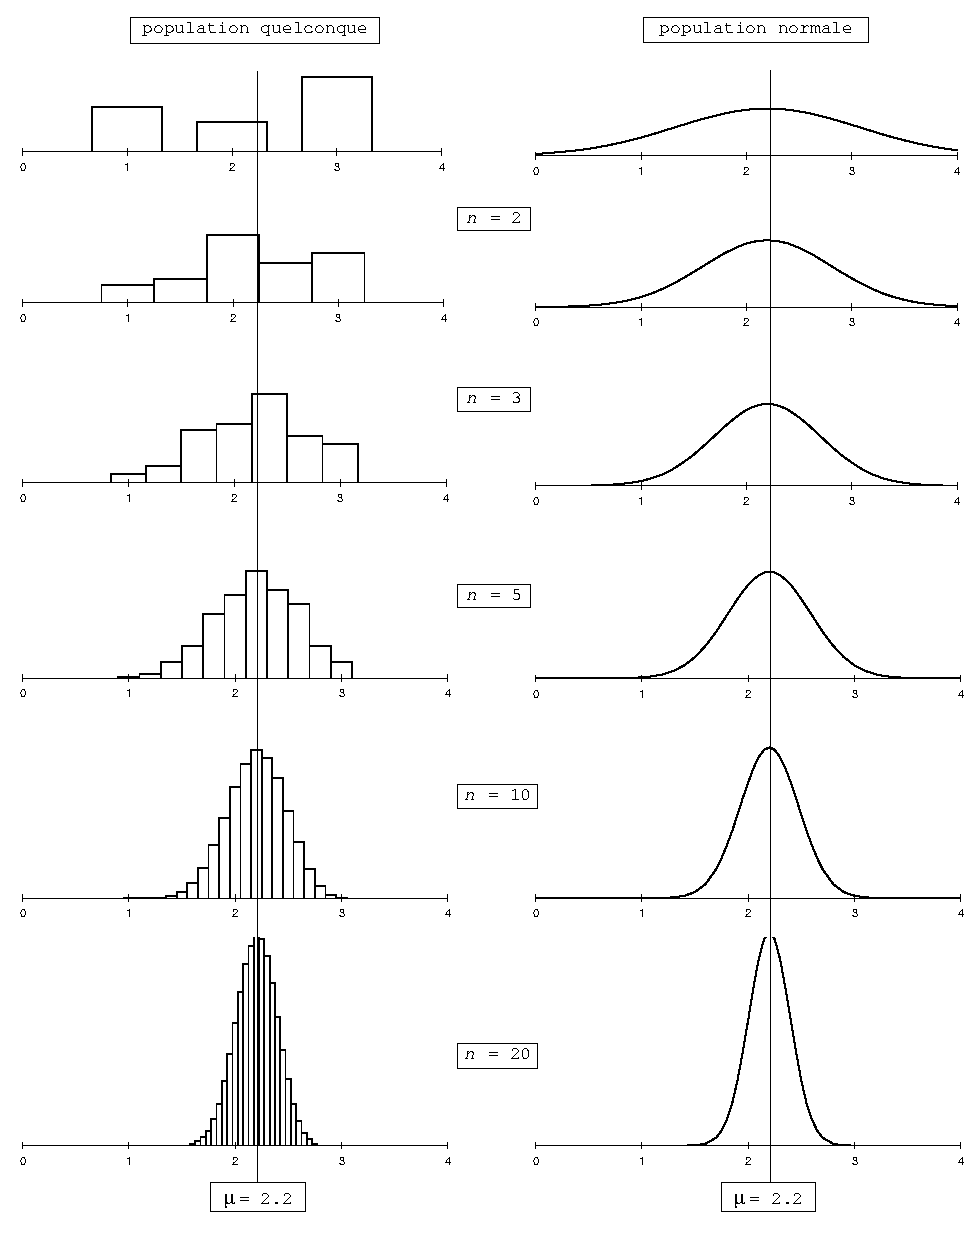
\includegraphics[width=14cm,clip]{central-limite}
  \caption{Distribution de $\overline{X}$ en fonction de la taille $n$ d'�chantillon.}
\end{figure}

\begin{theo}\label{theoCentralLimit}[Th�or�me central limite]
Soit une suite $(X_1, X_2, \ldots, X_n)$ de $n$ variables al�atoires identiquement et ind�pendamment distribu�es $(\mu,\sigma^2)$. Lorsque $n \rightarrow \infty$, la distribution de
$$\bar{X} = \frac{1}{n} \sum_i X_i$$
tend vers la loi $\norm\bigl(\mu, \frac{\sigma^2}{n}\bigr)$
\end{theo}

\begin{rem}
Plus la taille de l'�chantillon augmente, meilleure est l'approximation par la loi normale.
\end{rem}

En d'autres termes, pour des �chantillons de taille suffisamment grande, en pratique de taille au moins 30, on remarque que la distribution d'�chantillonnage a une forme en ''courbe en cloche''. Il s'agit de la loi de Gauss, ou loi normale. Un plan de sondage tr�s pr�cis correspond � une courbe tr�s peu �tal�e.  Si le plan de sondage est en plus tr�s peu biais�, alors le pic de la courbe est au voisinage de la vraie valeur du param�tre $\theta$.

%\begin{exo} En classe
%\begin{itemize}
%	\item Chaque �tudiant joue 10 fois � pile ou face et inscrit la proportion de piles. Faire un graphique de la distribution de $p$= proportion de piles.
%  \item Chaque �tudiant indique un budget pour ses soir�es et les donn�es sont r�colt�es afin de d�terminer le budget moyen, � l'aide d'�chantillons. Les budgets sont tri�s par ordre croissant. Quel �chantillon semble le plus repr�sentatif?
%\begin{enumerate}
%	\item Les 6 premiers budgets
%	\item Les 6 derniers budgets
%	\item les 6 valeurs centrales
%	\item 6 nombres pris au hasard
%\end{enumerate}
%Prendre 20 �chantillons de 6 budgets et repr�senter les valeurs des 20 moyennes d'�chantillons correspondants
%\end{itemize}
%Conclusion: Pour une population donn�e, les caract�ristiques d'un �chantillon issu de cette population fluctuent, d'un �chantillon � l'autre
%\end{exo}

Ainsi, pour $n$ suffisamment grand
$$\frac{\bar X-\mu}{\sigma/\sqrt{n}} = \frac{\bar X - \mu}{\sigma_{\bar X}}\;\; \stackrel{\text{\footnotesize app}}{\sim}\;\norm(0,1)$$
quelle que soit la distribution des $X_i$.

\newpage
\subsection{Distribution d'une proportion d'un �chantillon}
Remarquons qu'une proportion peut �tre vue comme une moyenne particuli�re, dans laquelle la variable d'investigation vaut 1 si la caract�ristique recherch�e est pr�sente, et 0 sinon. Une telle variable est appel�e variable bool�enne, ou dichotomique.

Notations:

\begin{tabular}{cl}
	$X$ & nombre d'individus dans la population avec la caract�ristique\\
	$N$ & taille de la population\\
	$x$ & nombre d'individus dans l'�chantillon avec la caract�ristique\\
	$n$ & taille de l'�chantillon\\
	$\pi=\frac{X}{N}$ & proportion d'individus dans la population ayant la caract�ristique\\
	$\bar{p}=\frac{x}{n}$ & proportion d'individus dans l'�chantillon avec la caract�ristique\\
	$\bar{p}-\pi$ & erreur d'�chantillonnage
\end{tabular}

Si la taille de l'�chantillon est suffisamment grande, en pratique, si
$$n\pi\geq 5\quad\quad\mbox{ et } n(1-\pi)\geq 5$$
alors la distribution normale peut �tre utilis�e.

\begin{theo}
Lorsque la taille de l'�chantillon est suffisamment grande, en pratique si $n\pi\geq 5$ et $n(1-\pi)\geq 5$, alors la distribution d'�chantillonnage de la proportion $\bar{p}$ est caract�ris�e par\\
\begin{center}
\begin{tabular}{c|c}
	Moyenne & \'Ecart-type\\
	\hline
	$\mu_{\bar{p}}=\pi$ & $\sigma_{\bar{p}}=\sqrt{\frac{\pi(1-\pi)}{n}}$
\end{tabular}
\end{center}

\begin{tabular}{cl}
$\pi$ & proportion dans la population\\
$n$ & taille de l'�chantillon\\
$\bar{p}$ & proportion dans l'�chantillon
\end{tabular}
\end{theo}

\begin{ex}
Le responsable d'une agence immobili�re souhaite passer une annonce vantant la rapidit� de traitement des affaires. Il pense que le 80\% des propri�t�s � vendre trouvent preneur en au plus 4 mois. Il a s�lectionn� al�atoirement 100 affaires, et parmi celles-l�, 73 se sont termin�es en au plus 4 mois. Les �tapes suivantes d�terminent la probabilit� de ce r�sultat:
\begin{enumerate}
	\item D�terminer la proportion de la population.\\
	La population est suppos�e avoir une proportion de 0.8, bas�e sur l'intuition du manager.
	\item Calculer la proportion de l'�chantillon.\\
	$$\bar{p}=\frac{73}{100}$$
	\item D�terminer la moyenne et l'�cart type de la distribution d'�chantillonnage.\\
	$$\mu_{\bar{p}}=0.8 \quad \sigma_{\bar{p}}=\sqrt{\frac{\pi(1-\pi)}{n}}=\sqrt{\frac{0.8(1-0.8)}{100}}=0.04$$
	\item D�finir l'�v�nement d'int�r�t.\\
	$$P(\bar{p}\leq 0.73)=?$$
	\item V�rifier les hypoth�ses.\\
	Comme $n\pi=80$ et $n(1-\pi)=20$ sont suffisamment grands (sup�rieurs � 5), convertir $\bar{p}$ en la variable centr�e r�duite $z$
	 $$z=\frac{\bar{p}-\pi}{\sigma_{\bar{p}}}=\frac{0.73-0.8}{\sqrt{\frac{0.8(1-0.8)}{100}}}=-1.75$$
	\item D�terminer la probabilit�.\\
	$$P(\bar{p}\leq 0.73)=P(z\leq -1.75)=0.0401$$
\end{enumerate}
Ainsi, il y a seulement 4\% de chance que sur un �chantillon al�atoire de taille 100, 73 affaires ou moins trouvent preneur en au plus 4 mois.
\end{ex}

%\begin{exo}
%Lors d'une �lection, $\theta=p=20\%$ des �lecteurs choisissent le candidat Schroumpf. Un institut de sondage interroge au pr�alable certains �lecteurs choisis au hasard. Soit $X$ la variable al�atoire valant 1 si l'�lecteur vote pour Schroumpf, et 0 sinon.\\
%Quelle loi suit la variable al�atoire $X$?\\
%Une loi de Bernoulli  de param�tre $p=0.2$\\
%On interroge $n=100$ �lecteurs par un tirage avec remise (ou sans remise si le nombre total d'�lecteurs est suffisamment grand, car la loi hyperg�om�trique converge vers la loi binomiale dans ce cas).
%Le nombre de votes favorables � Schroumpf est donc $X_1+\ldots + X_{100}$. Ce nombre est une variable al�atoire qui suit une loi binomiale $\bin(100,0.2)$
%La proportion de votants pour Schroumpf est la valeur de la variable al�atoire
%$$\hat{p}=\frac{X_1+\ldots +X_{100}}{100}$$
%dont l'esp�rance est $\E(\hat{p})= 0.2$
%et la variance $\var(\hat{p})=0.0016$\\
%Par le th�or�me central limite, la loi de $\hat{p}$ est donc proche d'une loi normale
%$\norm (0.2,0.0016)$\\
%
%Rappel du Th�or�me de la Limite Central\\
%Si $X_1 , X_2 , X_3 , \ldots , X_n$ sont des variables al�atoires ind�pendantes, de m�me loi de probabilit�, d'esp�rance $\mu$ et de variance $\sigma^2$, la loi de probabilit� de $$\frac{X_1 + X_2 +  \ldots + X_n-n\mu}{\sigma\sqrt{n}}$$
%tend, quand $n\to\infty$ , vers la loi normale centr�e r�duite.\\
%
%Conclusion:
%$$E(\hat{p})=p\quad\quad V(\hat{p})=\frac{p(1-p)}{n}$$
%A la limite, si $n\to\infty$, alors $V(\hat{p})\to 0$ et $\hat{p}\to p$\\
%La fr�quence observ�e $\hat{p}$ tend vers la proportion $p$ de la population lorsque $n$ tend vers l'infini.
%\end{exo}

%%%%%%%%%%%%%%%%%%%%%%%%%%%%%%%%%%%%%%%%%%%%%%
%%                                          %%
%%     Estimation par intervalle            %%
%%                                          %%
%%%%%%%%%%%%%%%%%%%%%%%%%%%%%%%%%%%%%%%%%%%%%%
\section{Intervalle de confiance}
Une estimation ponctuelle attribue une valeur pr�cise � un param�tre, mais engendre le risque que la valeur ainsi obtenue soit relativement �loign�e de la r�alit�. L'id�e de l'estimation par intervalle est de calculer un intervalle dans lequel se trouve la valeur du param�tre cherch�, avec un niveau de confiance fix�.

Soit un param�tre $\theta$. Au lieu de fournir une estimation $\hat{\theta}$, on construit un intervalle de valeurs de la forme
$$\left[\hat{\theta}_{inf} \; ; \; \hat{\theta}_{sup}\right]$$
dans lequel la vraie valeur du param�tre a une certaine probabilit� fix�e � l'avance, not�e $1-\alpha$, de se trouver.

% %------------------------------------
% \begin{center}
% 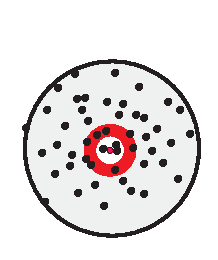
\includegraphics[width=7cm]{cible_abs_biais} \hfill
% 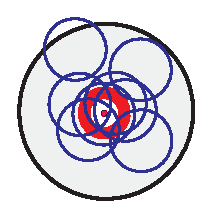
\includegraphics[width=7cm]{cible_interv}
% \hspace*{8ex} Estimations ponctuelles \hfill Estimations par intervalle \hspace*{5ex}
% \end{center}
% %------------------------------------
%

%------------------------------------
\begin{center}
\begin{tabular}{cc}
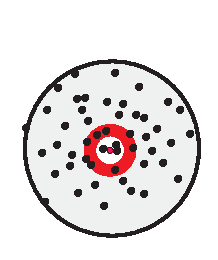
\includegraphics[scale=1.4]{cible_abs_biais}
&
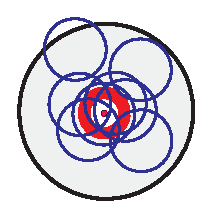
\includegraphics[scale=1.4]{cible_interv}\\
Estimations ponctuelles & Estimations par intervalle%
\end{tabular}
\end{center}	
 %------------------------------------

\begin{defi}
$1-\alpha$ est appel� le \emph{degr� de confiance} ou \emph{niveau de confiance}; il indique la probabilit� que l'intervalle de confiance recouvre la vraie valeur  $\theta$ du param�tre.\\
$$    \underbrace{1-\alpha}_{\parbox{3cm}{\centering\small degr� de
    confiance}}
    = \; P\bigl(\;\theta \in
    \underbrace{
    [\hat\theta_{\text{inf}}\;;\;\hat\theta_{\text{sup}}]
    }_{\text{\small intervalle al�atoire}}\bigr)\quad
$$
\end{defi}

\begin{defi}
Le \emph{risque de premi�re esp�ce} $\alpha$ est le risque que l'intervalle ne recouvre pas $\theta$.
\end{defi}

Le choix du degr� de confiance est crucial, car il influence
directement l'utilit� des r�sultats:
\begin{itemize}
    \item Si $\alpha$ est tr�s petit, l'intervalle est tr�s fiable, mais il devient tellement grand qu'il ne nous renseigne plus de fa�on utile sur la vraie valeur du param�tre.
    \item Si $\alpha$ est tr�s grand, l'intervalle est tr�s pr�cis (= �troit), mais la probabilit� qu'il recouvre effectivement la vraie valeur du param�tre est faible.
\end{itemize}

En pratique, on choisit g�n�ralement un risque $\alpha$ de 5\% ou de 10 \%.

\begin{defi}
Un \emph{intervalle de confiance} de niveau $1 - \alpha$ pour un param�tre inconnu $\theta$ d'une population est un intervalle tel que la probabilit� pour que cet intervalle recouvre $\theta$ est $1 - \alpha$. 
\end{defi}

Les bornes de cet intervalle se calculent � partir d'un �chantillon.

\subsection{Construction d'un intervalle de confiance}
Tout intervalle de confiance se construit selon le sch�ma suivant:
\begin{center}
Estimation ponctuelle $\pm$ (Valeur critique) $\cdot$ (\'Ecart type)
\end{center}

 \begin{center}
    \setlength{\unitlength}{1cm}
    \begin{picture}(8,1.8)(0,-0.8)
        \thicklines
        \put(0,0){\line(1,0){8}}
        \put(0,-.50){\line(0,1){.6}}
        \put(0,-1){\parbox[t]{0em}{\makebox[0pt][c]{$\hat{\theta}_{\text{inf}}$}}}
        \put(4,-.50){\line(0,1){.6}}
        \put(4,0.5){\parbox[t]{0em}{\makebox[0pt][c]{Estimation ponctuelle}}}
        \put(4,-1){\parbox[t]{0em}{\makebox[0pt][c]{$\hat{\theta}$}}}
        \put(8,-.50){\line(0,1){.6}}
        \put(8,-1){\parbox[t]{0em}{\makebox[0pt][c]{$\hat{\theta}_{\text{sup}}$}}}
    \end{picture}
  \end{center}

Apr�s avoir d�cid� du degr� de confiance � utiliser, la construction d'un intervalle de confiance pour un param�tre  $\theta$ quelconque s'effectue en suivant les 3 �tapes suivantes:

\begin{enumerate}
  \item Choix d'une statistique dont la distribution est connue.
		$$f(\theta) \sim \cal{D}$$
 		\textit{Remarque: Le param�tre pour lequel on construit l'intervalle de confiance doit pouvoir �tre explicit� � partir de la distribution choisie.}
  \item Construction de l'intervalle pour la statistique choisie:
		$$\left[\cal{D}_{\text{inf}} \; ; \; \cal{D}_{\text{sup}}\right]$$
  \item Construction de l'intervalle pour le param�tre:
		$$\left[\hat{\theta}_{\text{inf}} \; ; \; \hat{\theta}_{\text{sup}}\right]$$
\end{enumerate}

Nous allons tout d'abord �tudier l'intervalle de confiance pour estimer une moyenne. Deux cas peuvent se pr�senter: soit la variance (ou l'�cart type) de la population est connue, soit elle ne l'est pas. Ensuite, nous �tudierons l'intervalle de confiance pour une proportion, et finalement pour une variance.

%\newcommand{\MyNode}[2][cyan]{\Tr{\psshadowbox[fillcolor=#1]{\makebox[4cm]{\color{blue}#2}}}}
%\psset{treesep=2.5}
%  \begin{psmatrix}[mnode=r,colsep=-0.2]
%                      & & \MyNode[red!10]{Intervalle de Confiance}\\
%    & \MyNode[red!10]{Moyenne} && \MyNode[red!10]{Proportion}\\
%    \MyNode[red!10]{$\sigma^2$ connu} && \MyNode[red!10]{$\sigma^2$ inconnu}
%  \end{psmatrix}
%  \ncangle[angleA=-90,angleB=90]{1,3}{2,2}
%  \ncangle[angleA=-90,angleB=90]{1,3}{2,4}
%  \ncangle[angleA=-90,angleB=90]{2,2}{3,1}
%  \ncangle[angleA=-90,angleB=90]{2,2}{3,3}

%\newcommand{\MyNode}[2][cyan]{\Tr{\psshadowbox[fillcolor=#1]{\makebox[4cm]{\color{blue}#2}}}}
%\psset{treesep=2.5}
%  \begin{psmatrix}[mnode=r,colsep=-0.2]
%                      & & \MyNode[red!10]{Intervalle de Confiance}\\
%    & \MyNode[red!10]{Moyenne} && \MyNode[red!10]{Proportion}\\
%    \MyNode[red!10]{$\sigma^2$ connu} && \MyNode[red!10]{$\sigma^2$ inconnu}
%  \end{psmatrix}
%  \ncangle[angleA=-90,angleB=90]{1,3}{2,2}
%  \ncangle[angleA=-90,angleB=90]{1,3}{2,4}
%  \ncangle[angleA=-90,angleB=90]{1,3}{2,5}
%  \ncangle[angleA=-90,angleB=90]{2,2}{3,1}
%  \ncangle[angleA=-90,angleB=90]{2,2}{3,3}

$$
\begin{tikzpicture}[
%	% Label style
    label distance=1mm,
    every label/.style={blue},
	% Event style
    event/.style={rectangle,thick,draw,fill=yellow!20,
		text centered,font=\sffamily,anchor=north},
% Children and edges style
    edge from parent/.style={very thick,draw=black!70},
    edge from parent path={(\tikzparentnode.south) -- ++(0,-1.05cm)
			-| (\tikzchildnode.north)},
    level 1/.style={sibling distance=3cm,level distance=1.4cm,
			growth parent anchor=south,nodes=event},
    level 2/.style={sibling distance=3cm},
%%  For compatability with PGF CVS add the absolute option:
%   absolute
    ]
%% Draw events and edges
    \node (g0) [event] {Intervalle de Confiance}
	     	   child { node (g1) {Moyenne}
	     	      	child {node (g11) {$\sigma^2$ connu}}
	     	      	child {node (g12) {$\sigma^2$ inconnu}}
	     	      	}
	     	   	child { node (g2) {Proportion} }
	     	   	child { node (g3) {Variance}
	     	      	child {node (g31) {$\mu$ connu}}
	     	      	child {node (g32) {$\mu$ inconnu}}
	     	      	};
\end{tikzpicture}
$$

%%%%%%%%%%%%%%%%%%%%%%%%%%%%%%%%%%%%%%%%%%%%%%
%%                                          %%
%%    IC de mu, sigma connu                 %%
%%                                          %%
%%%%%%%%%%%%%%%%%%%%%%%%%%%%%%%%%%%%%%%%%%%%%%
\section{IC pour estimer $\mu$, $\sigma^2$ connu}
Lorsque la population dont on cherche � estimer la moyenne suit une loi normale de variance $\sigma^2$ connue, l'intervalle de confiance est calcul� de la mani�re suivante:

$$\bar{x}\pm z_{\alpha/2} \frac{\sigma}{\sqrt{n}}$$
o�:\\
\begin{tabular}{ccl}
$\bar{x}$ & = & moyenne de l'�chantillon\\
$z_{\alpha/2}$ &= &  valeur critique de la distribution normale standard\\
& & pour un degr� de confiance de $1-\alpha$\\
$\sigma$ &= &  �cart type de la population\\
$n$ &= &  taille de l'�chantillon
\end{tabular}


\begin{ex}
Consid�rons la population suivante: l'ensemble des pots de peinture de 1lt remplis par une machine industrielle.
Supposons que la quantit� de peinture soit une variable al�atoire $X$ suivant une loi normale d'�cart type $\sigma=0.04$lt. Votre but en tant que responsable qualit� est de contr�ler qu'en moyenne, la machine remplisse 1lt de peinture par pot.

Vous pr�levez 4 pots de peinture au hasard et mesurez la quantit� de peinture dans chaque pot:

\begin{center}
\begin{tabular}{c|cccc}
	Pot & $x_1$ & $x_2$ & $x_3$ & $x_4$\\
	\hline
	Quantit� [lt] & 1.0 & 0.98 & 1.1 & 1.1
\end{tabular}
\end{center}

Vous voulez conna�tre l'intervalle de confiance � 95\% pour la quantit� de peinture par pot.
\begin{enumerate}
	\item La population d'int�r�t est l'ensemble des pots de peinture d'1lt remplis par la machine
	\item Le degr� de confiance $1-\alpha$ vaut 0.95. Donc $\alpha  = 0.05$
	\item La moyenne de l'�chantillon est $\bar{x}=\frac{1.0+0.98+1.1+1.1}{4}=1.045$
	\item L'erreur standard de la moyenne (=�cart type de l'estimateur) vaut
	$$\sigma_{\bar{x}} = \frac{0.04}{\sqrt{4}}=0.02$$
	\item Les pots peuvent �tre trop peu remplis, ou trop remplis. L'erreur de premi�re esp�ce $\alpha$ est alors divis�e en 2 parties.
	La valeur critique est donc $z_{\alpha/2}=z_{0.025}=1.96$
	\item L'intervalle de confiance est
	$$\bar{x}\pm z_{\alpha/2}\frac{\sigma}{\sqrt{n}} = 1.045\pm 1.96\cdot 0.02 = [1.0058;1.0842]$$
\end{enumerate}
Comme l'intervalle de confiance ne comprend pas la valeur de 1lt, vous concluez que la machine n'est pas bien r�gl�e car elle remplit trop les pots en moyenne.
\end{ex}

Les �tapes suivantes permettent de calculer l'intervalle de confiance estim� pour une moyenne de population, lorsque l'�cart type de la population est connue, et la moyenne suit une loi normale ou lorsque l'�chantillon est de taille au moins 30.
\begin{enumerate}
	\item D�finir la population d'int�r�t et s�lectionner un �chantillon al�atoire de taille $n$
	\item Sp�cifier le degr� de confiance $1-\alpha$
	\item Calculer la moyenne de l'�chantillon
	$$\bar{x}=\frac{\sum x_i}{n}$$
	\item D�terminer l'erreur standard de la moyenne
	$$\sigma_{\bar{x}} = \frac{\sigma}{\sqrt{n}}$$
	\item D�terminer la valeur critique $z_{\alpha/2}$
	\item Calculer l'intervalle de confiance
	$$\bar{x}\pm z_{\alpha/2}\frac{\sigma}{\sqrt{n}}$$
\end{enumerate}

%%%%%%%%%%%%%%%%%%%%%%%%%%%%%%%%%%%%%%%%%%%%%%
%%                                          %%
%%    Estimation de mu, sigma inconnu       %%
%%                                          %%
%%%%%%%%%%%%%%%%%%%%%%%%%%%%%%%%%%%%%%%%%%%%%%
\section{IC pour estimer $\mu$, $\sigma^2$ inconnu}
Consid�rons l'\emph{hypoth�se suivante}: {\textcolor{red}{la distribution de la population suit une loi normale}.\\
Dans la plupart des cas o� la moyenne de la population est inconnue, la variance de la population est aussi inconnue. Il est alors n�cessaire d'estimer la variance de la population � l'aide de l'�chantillon. Il faut alors modifier la fa�on dont sont calcul�s la valeur critique et l'�cart type.

$$\bar{x}\pm t_{\alpha/2, n-1} \frac{s}{\sqrt{n}}$$
o�:\\
\begin{tabular}{ccl}
$\bar{x}$ & = & moyenne de l'�chantillon\\
$t_{\alpha/2, n-1}$ &= &  valeur critique de la $t$-distribution � $n-1$ degr�s de libert� \\
& & pour un degr� de confiance de $1-\alpha$\\
$s$ &= &  �cart type de l'�chantillon\\
$n$ &= &  taille de l'�chantillon
\end{tabular}

%\begin{ex}
%Consid�rons une population dont la moyenne est $\mu=2.5$ et le variance $\sigma^2=3$ pour une variable quantitative.
%
%{\itshape Echantillon} $X$:
% \begin{tabular}{lcccccccc}
%  $x_1$ & $x_2$ & $x_3$ & $x_4$ & $x_5$ & $x_6$
%& $x_7$ & $x_8$\\
% \hline
% 1 & 3 & 2 & 4 & 4 & 1 & 2 & 6
% \end{tabular}
%
%La moyenne de l'�chantillon $X$ vaut $\overline{x} = 2.875$ et sa variance vaut $s_X^2=2.61$\\
%
% {\itshape Echantillon} $Y$:
% \begin{tabular}{lcccccccc}
%  $y_1$ & $y_2$ & $y_3$ & $y_4$ & $y_5$\\
% \hline
% 2 & 2 & 1 & 1 & 3
% \end{tabular}
%
%La moyenne de l'�chantillon $Y$ vaut $\overline{y} = 1.8$ et sa variance vaut $s_Y^2=0.56$
%
%Consid�rons un degr� de confiance fix� � $1-\alpha=95\%$. Ainsi $\alpha=5\%$
%
% \begin{enumerate}
% \item Choix de la statistique
% \begin{eqnarray*}
%    t^{(n-1)} &=& \dfrac{\bar X - \mu}{\hat\sigma_{\bar X}}\;\sim\;\st_{n-1}\\
%    \Longrightarrow \quad \mu &=& \bar X - \hat\sigma_{\bar X}\,t^{(n-1)}
% \end{eqnarray*}
%	avec $\hat\sigma_{\bar X} = s/\sqrt{n-1}$
% \item Intervalle pour la statistique
%		On r�partit le risque total $\alpha$ en deux parts �gales � $\alpha / 2=0.025$ et les valeurs des 2 seuils sont d�termin�es � partir de la table de la loi de Student.
% \begin{center}
% \includegraphics[width=10cm]{interv_sym_T}
% \end{center}
% 		$$P(t_{\mbox{inf}} < t < t_{\mbox{sup}}) = 1 - \alpha$$
%		$$\left[t_{\mbox{inf}}=t_{\frac{\alpha}{2}}^{(n-1)} \; ; \; t_{\mbox{sup}}=t_{1-\frac{\alpha}{2}}^{(n-1)}\right]$$
% \item Intervalle pour le param�tre\\
%		\'Etant donn� que la loi de Student est sym�trique, $t_{\frac{\alpha}{2}}^{(n-1)} = - t_{1-\frac{\alpha}{2}}^{(n-1)}$ et l'intervalle s'�crit
%		$$\mu = \bar X \pm \hat\sigma_{\bar X}\;t_{1-\frac{\alpha}{2}}^{(n-1)}$$
% \end{enumerate}
%
%{\itshape Echantillon $X$ (n=8):}
%$$\left[t_{0.025}^{(7)}=-2.365 \; ; \; t_{0.975}^{(7)}=2.365\right]$$
%  \begin{eqnarray*}
%  \hat\sigma_{\bar X} &=& \sqrt{s^2/(n-1)} = \sqrt{2.61/7} = 0.6106\\[2ex]
%        \mu & = & 2.875 \pm 0.6106 \cdot 2.365 = 2.875 \pm 1.444
%    \end{eqnarray*}
%$$\Longrightarrow \quad P(\mu \in \left[1.341 \; ; \; 4.319\right]) = 95\%$$
%
%{\itshape Echantillon $Y$ (n=5):}
%$$\left[t_{0.025}^{(4)}=-2.777 \; ; \; t_{0.975}^{(4)}=2.777\right]$$
% \begin{eqnarray*}
% \hat\sigma_{\bar X} &=& \sqrt{0.56/4} = 0.3742\\[2ex]
% \mu &=& 1.8 \pm 1.039
% \end{eqnarray*}
%$$\Longrightarrow \quad P(\mu \in \left[0.761 \; ; \; 2.839\right]) = 95\%$$
%\end{ex}

\begin{ex}\label{exICMoyenneStudent}
% cf \cite{Groebner2005} p.277 Heritage software
En tant que responsable d'un ''backoffice'' dans une entreprise, vous souhaitez calculer l'intervalle de confiance � 95\% du temps moyen pass� au t�l�phone par les employ�s du ''backoffice'' avec les clients. Vous avez recueilli les temps, en minutes, de 25 appels.
$$\begin{array}{ccccc}
	 7.1 & 13.6 &  1.4 &  3.6 & 1.9\\
	11.6 &  1.7 & 16.9 &  2.6 & 7.7\\
	12.4 & 11.0 &  3.7 & 14.6 & 8.8\\
	 8.5 &  6.1 &  3.3 &  6.1 & 6.9\\
	 0.4 & 11.0 &  0.8 &  6.4 & 9.1
\end{array}$$

\begin{enumerate}
	\item la population consiste en tous les appels des clients au ''backoffice'', et l'�chantillon contient les 25 dur�es s�lectionn�es au hasard.
	\item le niveau de confiance souhait� est de $1-\alpha=0.95$
	\item la moyenne vaut $\bar{x}\approx 7.088$ et l'�cart type vaut $s\approx 4.64$
	\item l'erreur standard de la distribution d'�chantillonnage vaut
	$$\sigma_{\bar{x}}=\frac{s}{\sqrt{n}}\approx 0.928$$
	\item Comme vous ne savez pas � priori si la population est normalement distribu�e, vous v�rifiez � l'aide d'une bo�te � moustache que la distribution de votre �chantillon soit normalement distribu�e:\\
	% avec R
	%% x <- c(7.1,13.6,1.4,3.6,1.9,11.6,1.7,16.9,2.6,7.7,12.4,11,3.7,14.6,8.8,8.5,6.1,3.3,6.1,6.9,0.4,11,0.8,6.4,9.1)
	%% boxplot(x,main="Dur�e des appels", horizontal=TRUE)
	%% setwd("C:/Documents and Settings/Varone/Mes documents/Cours/Stat_III/fig")
	%% dev.copy2eps(file="exICstudent.eps")
	$$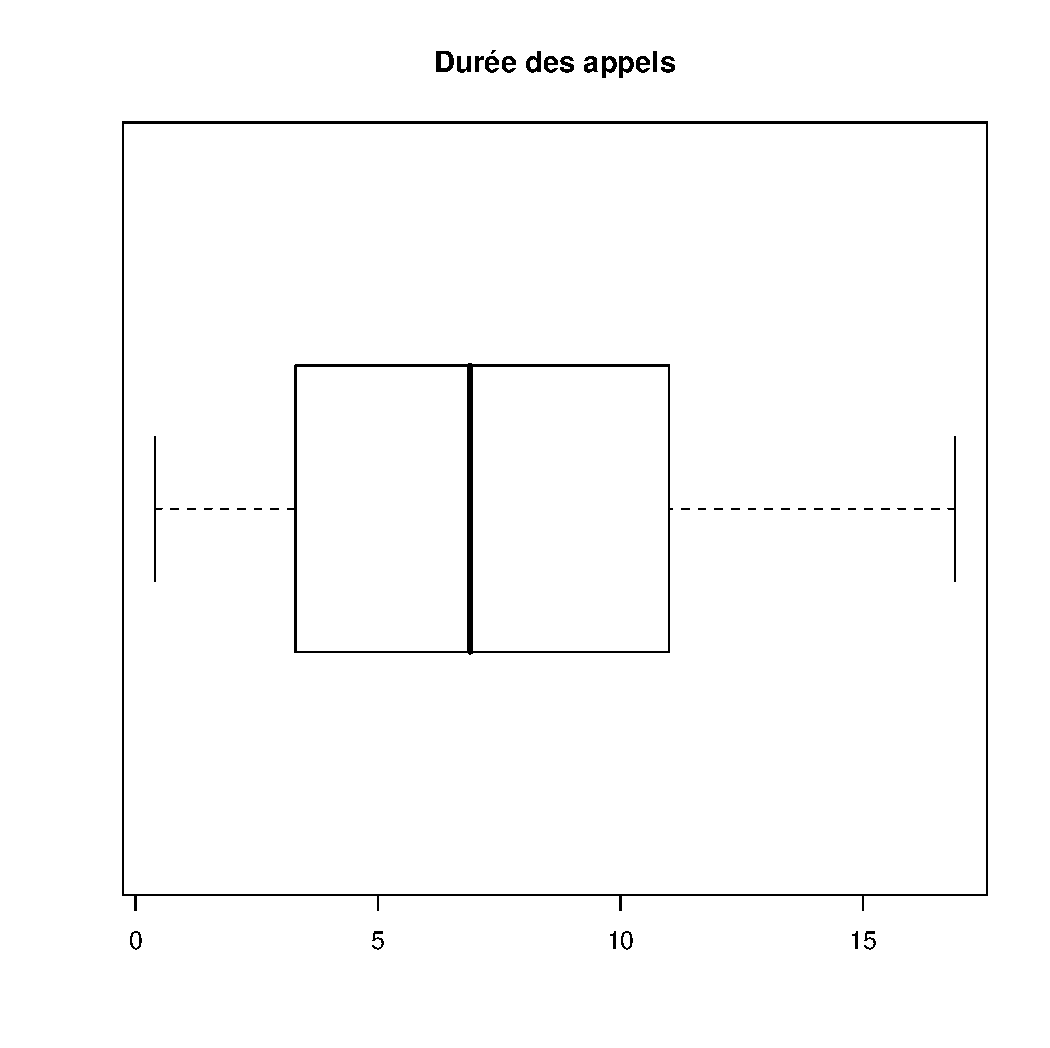
\includegraphics[scale=0.5]{exICstudent}$$
	la valeur critique vaut $t_{0.025,24} = 2.0639$
	\item l'intervalle de confiance vaut alors
	$$7.088\pm 2.0639\cdot 0.928 \ i.e.\ [5.173;9.003]$$
	%% t.test(x)
\end{enumerate}
\end{ex}

Les �tapes suivantes permettent de calculer l'intervalle de confiance estim� pour une moyenne de population, lorsque la variance de la population est inconnue, mais que la population est distribu�e suivant une loi normale,  et avec des �chantillons de petite taille (<30).
\begin{enumerate}
	\item D�finir la population d'int�r�t et s�lectionner un �chantillon al�atoire de taille $n$
	\item Sp�cifier le degr� de confiance $1-\alpha$
	\item Calculer la moyenne et l'�cart type de l'�chantillon
	$$\bar{x}=\frac{\sum x_i}{n}\quad s=\sqrt{\frac{\sum(x_i-\bar{x})^2}{n-1}}$$
	\item D�terminer l'erreur standard de la moyenne
	$$\sigma_{\bar{x}} = \frac{s}{\sqrt{n}}$$
	\item D�terminer la valeur critique $t_{\alpha/2,n-1}$
	\item Calculer l'intervalle de confiance
	$$\bar{x}\pm t_{\alpha/2,n-1}\sigma_{\bar{x}}$$
\end{enumerate}

\begin{rem}
Sous R (version 2.9.1) vous pouvez utiliser la fonction {\it t.test()} pour trouver l'intervalle de confiance.
\end{rem}

\begin{rem}
Lorsque l'�chantillon est de grande taille, c'est � dire de taille au moins 30, la statistique de test peut �tre approch�e � l'aide d'une $z$-valeur. On peut donc dans ce cas utiliser la formule suivante pour calculer l'intervalle de confiance:
 $$\bar{x}\pm z_{\alpha/2} \frac{s}{\sqrt{n}}$$
o�:\\
\begin{tabular}{ccl}
$\bar{x}$ & = & moyenne de l'�chantillon\\
$z_{\alpha/2}$ &= &  valeur critique de la distribution normale standard\\
& & pour un degr� de confiance de $1-\alpha$\\
$s$ &= &  �cart type de l'�chantillon\\
$n$ &= &  taille de l'�chantillon
\end{tabular}
\end{rem}

%%%%%%%%%%%%%%%%%%%%%%%%%%%%%%%%%%%%%%%%%%%%%%
%%                                          %%
%%    IC d'une proportion                   %%
%%                                          %%
%%%%%%%%%%%%%%%%%%%%%%%%%%%%%%%%%%%%%%%%%%%%%%
\section{IC pour estimer une proportion}
Lorsque la variable d'int�r�t est une proportion, il est aussi possible d'utiliser le th�or�me central limite  \ref{theoCentralLimit}, car une proportion n'est rien d'autre qu'une moyenne particuli�re: la variable d'investigation vaut 1 si la caract�ristique recherch�e est pr�sente, et 0 sinon.

\begin{ex}
$Y_i = \left\{
\begin{array}{ll}
	1 & \mbox{la personne a l'intention d'acheter le produit}\\
	0 & \mbox{sinon}
\end{array}
\right.$
\\[4pt]
$Y_i = \left\{
\begin{array}{ll}
	1 & \mbox{la personne a l'intention de voter pour Mme L.U.}\\
	0 & \mbox{sinon}
\end{array}
\right.$
\\[4pt]
$Y_i = \left\{
\begin{array}{ll}
	1 & \mbox{le client est satisfait du service}\\
	0 & \mbox{sinon}
\end{array}
\right.$
\end{ex}

\begin{theo}
Dans un sondage al�atoire simple, la proportion dans l'�chantillon $\bar{p}$ est un estimateur sans biais de la proportion $\pi$ dans la population.
\end{theo}

\begin{theo}
Lorsque la taille $n$ de l'�chantillon est suffisamment grande, i.e.
$n\pi\geq 5$ et $n(1-\pi)\geq 5$, la distribution d'�chantillonnage peut �tre approch�e par une distribution normale centr�e en $\pi$, avec comme �cart type
$$\sigma_{\bar{p}}=\sqrt{ \frac{\pi(1-\pi)}{n} }$$
o�\\
\begin{tabular}{rcl}
$\pi$ & = & proportion dans la population\\
$n$ & = & taille de l'�chantillon
\end{tabular}
\end{theo}

Comme le param�tre $\pi$ n'est pas connu,  il est alors simplement estim� par $\bar{p}$.

L'intervalle de confiance pour une proportion s'�crit donc, sous l'hypoth�se que la taille de l'�chantillon soit suffisamment grande:
$$\bar{p}\pm z_{\alpha/2}\sqrt{ \frac{\bar{p}(1-\bar{p})}{n} }$$
o�\\
\begin{tabular}{rcl}
$\bar{p}$ & = & proportion dans l'�chantillon\\
$\pi$ & = & proportion dans la population\\
$n$ & = & taille de l'�chantillon\\
$z_{\alpha/2}$ &= &  valeur critique de la distribution normale standard\\
& & pour un degr� de confiance de $1-\alpha$\\
\end{tabular}

\begin{ex}
Une entreprise r�unissant plusieurs marques d�sire estimer la proportion de ses clients connaissant plus de 5 de leur marques. Elle veut un degr� de confiance de 0.9. Elle effectue alors un sondage al�atoire parmi 100 clients et obtient comme estimation ponctuelle 0.2.
\begin{enumerate}
	\item La population d'int�r�t est l'ensemble de ses clients.
	\item L'�chantillon al�atoire s�lectionn� est suffisamment grand si la proportion cherch�e est entre 0.05 et 0.95, ce qui est le cas ici.
	\item Le degr� de confiance est $1-\alpha=0.9$
	\item La valeur critique $z_{\alpha/2}=z_{0.05}=1.645$
 	\item La proportion estim�e est $\bar{p}=0.2$
	\item L'intervalle de confiance vaut donc
	$$0.2\pm 1.645\sqrt{ \frac{0.2(1-0.2)}{100} } = [0.134,0.266]$$
\end{enumerate}
\end{ex}


Les �tapes suivantes permettent de calculer l'intervalle de confiance estim� d'une proportion
\begin{enumerate}
	\item D�finir la population d'int�r�t et la variable dont on veut estimer la proportion.
	\item S�lectionner un �chantillon al�atoire de taille $n$ suffisamment grande, telle que
	$$n\bar{p}\geq 5 \quad\mbox{ et }\quad n(1-\bar{p})\geq 5$$
	\item Sp�cifier le degr� de confiance $1-\alpha$
	\item D�terminer la valeur critique $z_{\alpha/2}$  tir�e d'une loi normale centr�e r�duite
 	\item Calculer la proportion $\bar{p}$
	\item Calculer l'intervalle de confiance
	$$\bar{p}\pm z_{\alpha/2}\sqrt{ \frac{\bar{p}(1-\bar{p})}{n} }$$
\end{enumerate}


%%%%%%%%%%%%%%%%%%%%%%%%%%%%%%%%%%%%%%%%%%%%%%
%%                                          %%
%%    Estimation de sigma^2, mu inconnnu    %%
%%                                          %%
%%%%%%%%%%%%%%%%%%%%%%%%%%%%%%%%%%%%%%%%%%%%%%
\section{IC pour estimer $\sigma^2$, $\mu$ inconnu}
\label{section:variance-estimation}

L'estimation de la variance d'une population est utilis�e par exemple pour mesurer la fiabilit� d'un site de production ou d'un fournisseur. La fiabilit� d'un instrument de mesure comme un altim�tre est cruciale: il n'est pas suffisant de savoir qu'un altim�tre donne en moyenne la bonne mesure (!) mais il faut aussi que les �carts par rapport � la moyenne soient suffisamment faibles.

La propri�t� \ref{pro:chi2} permet de calculer l'intervalle de confiance d'une variance:\\
\begin{eqnarray*}
\prob\left( q_{\inf} \leq Q_{n-1} \leq q_{\sup} \right) & = & 1-\alpha\\
\prob\left( \chi^2_{1-\alpha/2}\leq Q_{n-1} \leq \chi^2_{\alpha/2} \right) & = & 1-\alpha\\
\prob\left( \chi^2_{1-\alpha/2}\leq \frac{(n-1)s^2}{\sigma^2} \leq \chi^2_{\alpha/2} \right) & = & 1-\alpha\\
\prob\left( \frac{\chi^2_{1-\alpha/2}}{(n-1)s^2}  \leq \frac{1}{\sigma^2} \leq \frac{\chi^2_{\alpha/2}}{(n-1)s^2} \right) & = & 1-\alpha\\
\prob\left( \frac{(n-1)s^2}{\chi^2_{\alpha/2}}  \leq \sigma^2 \leq \frac{(n-1)s^2}{\chi^2_{1-\alpha/2}} \right) & = & 1-\alpha\\
\end{eqnarray*}

\begin{center}
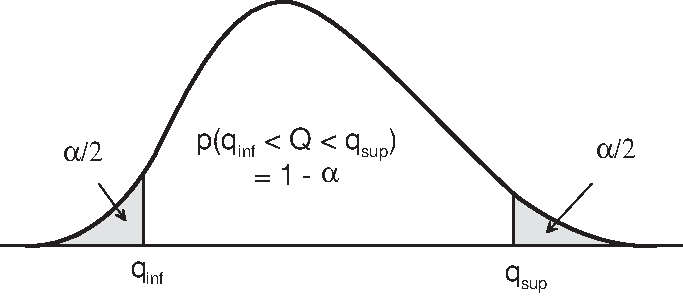
\includegraphics[width=10cm]{interv_stat_asym}
\end{center}

L'intervalle de confiance d'une variance s'�crit donc, sous l'hypoth�se que l'�chantillon al�atoire provient d'une population dont les �l�ments sont {\textcolor{red}{iid de distribution normale}:
$$\left[ \frac{(n-1)s^2}{q_{\alpha/2,n-1}}  ; \frac{(n-1)s^2}{q_{1-\alpha/2,n-1}} \right]$$
o�\\
\begin{tabular}{rcl}
$n$ & = & taille de l'�chantillon\\
$q_{\alpha/2,n-1}$ &= &  valeur critique de la distribution $\chi^2$ � $n-1$ degr�s de libert�\\
& & pour un degr� de confiance de $1-\alpha$\\
$s^2$ & = & variance de l'�chantillon\\
\end{tabular}

\begin{rem}
L'utilisation de la statistique du $\chi^2$ pour estimer la variance est tr�s sensible � une violation de l'hypoth�se d'une population normalement distribu�e. Cette technique n'est donc pas une technique robuste.
\end{rem}

\begin{ex}
% cf \cite{Groebner2005} p.388 H&L Machines
Une entreprise fabriquant des photocopieuses assure aussi le service apr�s-vente. Une nouvelle �quipe vient d'�tre form�e, et le responsable doit pr�voir l'affectation des services. Il veut en estimer avec un degr� de confiance de 0.9 le temps moyen de service et l'�cart type, afin de pouvoir planifier les services de la nouvelle �quipe. Pour cela, il inscrit la dur�e de 20 services pris al�atoirement parmi ceux effectu� par la nouvelle �quipe. Il calcule un �cart type de 0.5h et peut supposer que les donn�es proviennent d'une loi normale.

\begin{enumerate}
	\item La population d'int�r�t est l'ensemble des services effectu�s par la nouvelle �quipe.
	\item L'�chantillon s�lectionn� est de taille 20, et provient d'une population normalement distribu�e.
	\item Le degr� de confiance est de 0.9
	\item Les valeurs critiques sont $\chi^2_{0.05}=30.14$ et $\chi^2_{0.95}=10.12$ avec 19 degr�s de libert�.
	\item La variance estim�e est de $s^2=0.5^2=0.25$
	\item L'intervalle de confiance associ� � la variance est donc
$$\left[ \frac{(19)0.25}{30.14}  ; \frac{(19)0.25}{10.12} \right]
= [0.16;0.47]$$
\end{enumerate}
\end{ex}

%\begin{ex}
%Consid�rons une population dont la moyenne est $\mu=2.5$ et le variance $\sigma^2=3$ pour une variable quantitative.
%
%{\itshape Echantillon} $X$:
% \begin{tabular}{lcccccccc}
%  $x_1$ & $x_2$ & $x_3$ & $x_4$ & $x_5$ & $x_6$
%& $x_7$ & $x_8$\\
% \hline
% 1 & 3 & 2 & 4 & 4 & 1 & 2 & 6
% \end{tabular}
%
%La moyenne de l'�chantillon $X$ vaut $\overline{x} = 2.875$ et sa variance vaut $s_X^2=2.61$\\
%
% {\itshape Echantillon} $Y$:
% \begin{tabular}{lcccccccc}
%  $y_1$ & $y_2$ & $y_3$ & $y_4$ & $y_5$\\
% \hline
% 2 & 2 & 1 & 1 & 3
% \end{tabular}
%
%La moyenne de l'�chantillon $Y$ vaut $\overline{y} = 1.8$ et sa variance vaut $s_Y^2=0.56$
%
%Consid�rons un degr� de confiance fix� � $1-\alpha=95\%$. Ainsi $\alpha=5\%$
%
%{\itshape Echantillon $X$, $n$=8:}
%$$\left[q_{0.025}^{(7)}=1.69 \; ; \; q_{0.975}^{(7)}=16.01\right]$$
%$$\sum_i \;(x_i-\bar x)^2 = n\,s^2 = 8\cdot 2.61 = 20.88$$
%
%
%$$\Longrightarrow
%        \left[
%        \frac{20.88}{16.01}
%        \right.
%        ;
%        \left.
%        \frac{20.88}{1.69}
%        \right]
%        \quad = \quad
%        \left[
%        1.30
%        \right.
%        ;
%        \left.
%        12.36
%        \right]$$
%$$\Longrightarrow \mbox{ Intervalle pour }\sigma: \quad [1.14\;;\;3.52]$$
%
%{\itshape Echantillon $Y$, $n$=5:}
%$$\left[q_{0.025}^{(4)}=0.484 \; ; \; q_{0.975}^{(4)}=11.14 \right]$$
%$$\sum_i \;(x_i-\bar x)^2 = n\,s^2 = 5\cdot 0.56 = 2.80$$
%
%$$\Longrightarrow
%        \left[
%        \frac{2.80}{11.14}
%        \right.
%        ;
%        \left.
%        \frac{2.80}{0.484}
%        \right]
%        \quad = \quad
%        \left[
%        0.25
%        \right.
%        ;
%        \left.
%        5.79
%        \right]$$
%
%$$\Longrightarrow \mbox{ Intervalle pour }\sigma: \quad[0.50\;;\;2.41]$$
%\end{ex}

%{\itshape Remarque: La statistique $Q$ est une fonction monotone \textit{d�croissante} $g(\theta)$ de l'estim� $\theta$. Il en est de m�me de la transformation inverse $\theta=g^{-1}(Q)$ }
%
%$$Q_{(n)} = \frac{\sum_i \;(X_i-\mu)^2}{\sigma^2}
%        \quad \Leftrightarrow \quad \sigma^2 = \frac{\sum_i
%\;(X_i-\mu)^2}{Q_{(n)}}$$
% \vspace*{2ex}
%
% \begin{center}
% \parbox{10.2cm}{
% \includegraphics[width=8cm]{trsf_mono_decr}
%  }
% \ \parbox{5.5cm}{
% $q_{inf} \mapsto \theta_{sup}$
% \\[3ex]
% $q_{sup} \mapsto \theta_{inf}$
% }
% \end{center}

\section{R�sum�}
Le tableau suivant r�sume les distributions utilis�es pour repr�senter la moyenne, la proportion et la variance de la population:

\begin{center}
    \begin{tabular}{|c|l|c|}
    \hline&&\\[-1.5ex]
    estim�  & hypoth�se    & distribution
    \\[.5ex]
    \hline&&\\[-1ex]
    $\mu$   & $\sigma^2$ connu,  &\\
            & distr. normale ou $n\geq 30$
        & $Z =
%    \dfrac{\bar X-\mu}{\sigma/\sqrt{n}}=  \dfrac{\bar X-\mu}{\sigma_{\bar X}}\;\sim\norm (0,1)$
    \dfrac{\bar X-\mu}{\sigma/\sqrt{n}}\sim\norm (0,1)$
    \\[3ex]
  & $\sigma^2$ inconnu, distr. normale
     & $T_{(n-1)} =
%    \dfrac{\bar X - \mu}{s/\sqrt{n-1}}=\dfrac{\bar X - \mu}{\hat \sigma_{\bar X}} \; \sim\st_{n-1}$
    \dfrac{\bar X - \mu}{s/\sqrt{n}}\sim\st_{n-1}$
    \\[3ex]
    \hline&&\\[-1ex]
    $\pi$ & $n\pi\geq 5$ et $n(1-\pi)\geq 5$ &
    $Z=\frac{\bar{P}-\pi}{\sqrt{\frac{\pi(1-\pi)}{n}}}\sim\norm (0,1)$
    \\[3ex]
    \hline&&\\[-1ex]
    $\sigma^2$   & $\mu$ connu, distr. normale
    & $Q_{(n)}=\dfrac{\sum_{i=1}^{n} (X_i - \mu)^2}{\sigma^2} \;\sim\; \chi^2_n$
    \\[3ex]
     & $\mu$ inconnu, distr. normale
    & $Q_{(n-1)}=\dfrac{\sum_{i=1}^{n} (X_i - \bar X)^2}{\sigma^2}= \dfrac{(n-1)s^2}{\sigma^2} \;\sim\; \chi^2_{n-1}$
    \\[3ex]
    \hline
    \end{tabular}
\end{center}

Rappel: lorsque la population est distribu�e selon une loi quelconque de param�tres $\mu$ et $\sigma^2$, il est possible d'utiliser le th�or�me central limite \ref{theoCentralLimit}  pour estimer la moyenne, � condition que l'�chantillon utilis� soit de grande taille. En pratique, un �chantillon de taille au moins 30 suffit.

\begin{center}
    \begin{tabular}{|c|l|c|}
    \hline&&\\[-1.5ex]
    estim�  & hypoth�se    & intervalle \\[.5ex]
    \hline&&\\[-1ex]
    $\mu$   & $\sigma^2$ connu, &\\
            & distr. normale ou $n\geq 30$
            & $\mu \in \bar x \pm z_{\frac{\alpha}{2}}\frac{\sigma}{\sqrt{n}}$\\[3ex]
  & $\sigma^2$ inconnu, distr. normale
     & $\mu \in \bar x \pm t_{\frac{\alpha}{2},n-1}\frac{s}{\sqrt{n}}$\\[3ex]
    \hline&&\\[-1ex]
    $\pi$ & $n\bar{p}\geq 5$ et $n(1-\bar{p})\geq 5$ & $\bar{p}\pm z_{\alpha/2}\sqrt{ \frac{\bar{p}(1-\bar{p})}{n} }$ \\[3ex]
    \hline&&\\[-1ex]
    $\sigma^2$   & $\mu$ connu, distr. normale
    & $\left[ \frac{\sum (x_i - \mu)^2}{q_{\frac{\alpha}{2},n}}
        \;;\; \frac{\sum (x_i - \mu)^2}{q_{1-\frac{\alpha}{2},n}}
        \right]$\\[3ex]
     & $\mu$ inconnu, distr. normale
    & $\left[ \frac{\sum (x_i - \bar{x})^2}{q_{\frac{\alpha}{2},n-1}}
        \;;\; \frac{\sum (x_i - \bar{x})^2}{q_{1-\frac{\alpha}{2},n-1}}
        \right]$\\[4ex]
    \hline
    \end{tabular}
\end{center}

\chapter{Tests param�triques}

%%%%%%%%%%%%%%%%%%%%%%%%%%%%%%%%%%%%%%%%%%%%%%%
%%                                           %%
%%        Principe des tests                 %%
%%                                           %%
%%%%%%%%%%%%%%%%%%%%%%%%%%%%%%%%%%%%%%%%%%%%%%%
\section{Principe des tests d'hypoth�ses}
\begin{center}
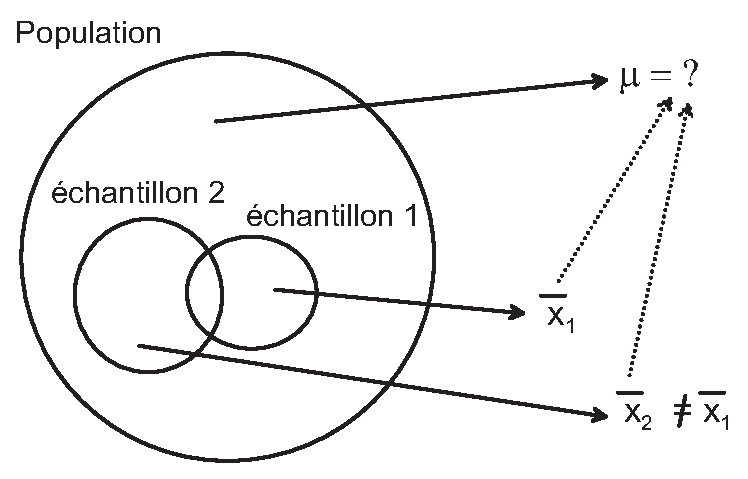
\includegraphics[width=9cm]{inference_2}
\end{center}
Le but de l'estimation est de quantifier, alors que le but d'un test est de valider/invalider une hypoth�se.
Pour cela, on proc�de de la mani�re suivante:
\begin{enumerate}
  \item On formule une hypoth�se sur la population ou sur la distribution �tudi�e.
  \item On v�rifie si l'�chantillon utilis� provient bien de la population ou de la distribution �tudi�e, avec un certain degr� de confiance.
\end{enumerate}
Le test statistique lui-m�me correspond � la r�gle de d�cision.\\

\begin{defi}
Les \emph{tests param�triques} pr�supposent que les donn�es sont distribu�es selon une loi particuli�re.
Le test s'effectue alors en comparant certains param�tres de la distribution, comme la moyenne ou la variance.
\end{defi}

\begin{defi}
Les \emph{tests non-param�triques} ne pr�supposent pas de distribution particuli�re des donn�es. Les tests s'effectuent en tirant des conclusions � partir des valeurs observ�es des �chantillons, sans faire appel � des param�tres tels que la moyenne ou la variance.
\end{defi}

Les tests non-param�triques ont un champ d'application plus large que les tests param�triques, car ils ne n�cessitent pas une distribution particuli�re des donn�es. En revanche, ils sont g�n�ralement moins puissants et le risque total d'erreur est plus grand.

\subsection{Hypoth�ses nulle et alternative}
Un test consiste � choisir entre deux hypoth�ses en fonction d'un �chantillon. L'hypoth�se nulle, $H_0$, est celle que l'on veut tester. L'hypoth�se alternative, $H_1$, est son ``contraire''.

\begin{defi}
L'\emph{hypoth�se nulle $H_0$} est l'affirmation au sujet d'un param�tre de la population, qui sera test�e. L'hypoth�se nulle sera rejet�e seulement si la statistique calcul�e � partir de l'�chantillon, apporte une contradiction suffisamment forte.
\end{defi}

\begin{defi}
L'\emph{hypoth�se alternative $H_1$} est l'ensemble des valeurs d'un param�tre de la population non couvert par l'hypoth�se nulle. L'hypoth�se alternative est r�put�e vraie si l'hypoth�se nulle est rejet�e.
\end{defi}

\begin{eqnarray*}
	H_0 &:& \mbox{hypoth�se nulle (� tester)}\\
	H_1 &:& \mbox{hypoth�se alternative}
\end{eqnarray*}

En fonction des hypoth�ses de d�part, le r�sultat d'un test est toujours univoque: soit il y a suffisamment d'�vidence pour rejeter l'hypoth�se nulle, soit il n'y en a pas suffisamment (et donc \emph{a fortiori} acceptation de l'hypoth�se nulle).

\begin{ex}
% Exemple d'Andre Berchtold transform�
On suppose que les petites entreprises suisses ont en moyenne 35 employ�s avec une variance �gale � 220.
Un �chantillon al�atoire de taille 20 a donn� un nombre moyen d'employ�s �gal � 27 et une variance de 334.7.

 \begin{center}
 \begin{tabular}{cccccccccc}
 2 & 2 & 5 & 6 & 7 & 8 & 12 & 14 & 23 & 26\\
 28 & 31 & 40 & 42 & 46 & 47 & 48 & 49 & 52 & 52
 \end{tabular}
 \end{center}

En fonction du r�sultat donn� par l'�chantillon, est-il statistiquement admissible que le nombre moyen d'employ�s dans l'ensemble des petites entreprises du pays soit r�ellement �gal � 35?
Pour r�pondre � cette question, il faut former l'hypoth�se nulle et l'hypoth�se alternative suivantes:
\begin{eqnarray*}
	H_0 &:& \mu=35\\
	H_1 &:& \mu\not=35
\end{eqnarray*}
\end{ex}

Les r�gles suivantes aident � formuler l'hypoth�se nulle et l'hypoth�se alternative:
\begin{enumerate}
	\item L'hypoth�se nulle et l'hypoth�se alternative doivent �tre formul�es en termes du param�tre de la population d'int�r�t.
	\item L'hypoth�se nulle repr�sente un statu quo. Elle repr�sente la condition qui est suppos�e exister, � moins qu'il n'y ait suffisamment d'�vidence montrant que la situation a chang�.
	\item L'hypoth�se nulle  doit contenir un signe d'�galit� $=$ ou $\geq$ ou $\leq$.
\end{enumerate}

\begin{ex}
Les �tudiants en emploi b�n�ficient d'un horaire tenant compte de leur situation, � savoir un travail de 25h par semaine, correspondant � un temps partiel de 60\%.  Afin de tenir compte au mieux de leur situation r�elle, le management d�sire savoir si la situation r�elle a chang�. Les �tapes suivantes permettent de formuler l'hypoth�se nulle et l'hypoth�se alternative:
\begin{enumerate}
	\item D�terminer le param�tre de la population d'int�r�t\\
	Le param�tre � consid�rer est le nombre d'heures de travail moyen par semaine des �tudiants en emploi.
	\item D�finir la situation qui est suppos�e vraie � moins qu'il y ait suffisamment d'�vidence que cela ne soit plus le cas.\\
	Le statu quo est de consid�rer que les �tudiants en emploi travaillent 25 heures ou moins par semaine en moyenne. S'il y a suffisamment d'�vidence que la moyenne est plus grande que 25h/semaine , alors cela impliquera un effort consid�rable de r�organisation. Dans ce dernier cas, il s'agit de rejeter le status quo.
	\item Formuler l'hypoth�se nulle et l'hypoth�se alternative\\
\begin{eqnarray*}
	H_0 &:& \mu\leq25\\
	H_1 &:& \mu>25
\end{eqnarray*}	
\end{enumerate}
\end{ex}

\begin{rem}
Une \emph{hypoth�se simple} correspond � une valeur sp�cifique, une situation d�termin�e (une hypoth�se sur une �galit�).
Une \emph{hypoth�se composite} correspond � un ensemble de valeurs, de situations (une hypoth�se sur une in�galit�).
\end{rem}

\subsection{R�gion critique et valeur critique}
Le principe du test est de rejeter l'hypoth�se $H_0$ si la valeur de la statistique $Q_0$ observ�e dans l'�chantillon est trop diff�rente de la valeur th�orique postul�e sous $H_0$ pour la population.

A cette fin, l'espace des valeurs possibles de la statistique $Q_0$ est divis� en deux zones:
\begin{itemize}
    \item $A$ : ensemble des valeurs probables de $Q_0$ lorsque l'hypoth�se $H_0$ est vraie.\\
    Il s'agit de la r�gion d'acceptation de $H_0$.
    \item $R$ : ensemble des valeurs peu probables de $Q_0$ lorsque l'hypoth�se $H_0$ est vraie.\\
    Il s'agit de la r�gion de rejet de $H_0$ (r�gion critique).
 \end{itemize}

\begin{center}
\fbox{\parbox{\linewidth}{
\textbf{R�gle de d�cision}
\begin{eqnarray*}
   q_0 \notin R & \Longleftrightarrow &
   \text{Acceptation}\text{ de } H_0\\[1ex]
   q_0 \in R & \Longleftrightarrow & \text{Rejet de } H_0
\end{eqnarray*}
}}
\end{center}

\textbf{Forme de la r�gion critique $R$}\\
La forme de la r�gion critique $R$ d�pend du type d'hypoth�se alternative retenue. On distingue les trois cas suivants:
\begin{itemize}
    \item
    \parbox[t]{.55\linewidth}{test unilat�ral � gauche\\$H_1$ : $q=q_1<q_0$}\quad
    %
    \setlength{\unitlength}{1cm}
    \begin{picture}(5,1)
        \thicklines
        \put(0,0.3){\line(1,0){5}}
        \put(1.5,0.5){\line(-1,-2){.2}}
        \put(1.2,0.5){\line(-1,-2){.2}}
        \put(.9,0.5){\line(-1,-2){.2}}
        \put(.6,0.5){\line(-1,-2){.2}}
        \put(.3,0.5){\line(-1,-2){.2}}
        \put(1.6,0.1){\parbox[t]{0em}{\makebox[0pt][c]{]}}}
        \put(3.3,.7){\parbox[t]{0em}{\makebox[0pt][c]{$A$}}}
        \put(.9,.7){\parbox[t]{0em}{\makebox[0pt][c]{$R$}}}
        \put(1.6,-0.6){\parbox[t]{0em}{\makebox[0pt][c]{$r$}}}
    \end{picture}\\[2ex]

  \item
    \parbox[t]{.55\linewidth}{test unilat�ral � droite\\$H_1$ :
$q=q_1>q_0$}\quad
    %
    \setlength{\unitlength}{1cm}
    \begin{picture}(5,1)
        \thicklines
        \put(0,0.3){\line(1,0){5}}
        \put(3.5,0.1){\line(1,2){.2}}
        \put(3.8,0.1){\line(1,2){.2}}
        \put(4.1,0.1){\line(1,2){.2}}
        \put(4.4,0.1){\line(1,2){.2}}
        \put(4.7,0.1){\line(1,2){.2}}
        \put(3.4,0.1){\parbox[t]{0em}{\makebox[0pt][c]{[}}}
        \put(3.4,-0.6){\parbox[t]{0em}{\makebox[0pt][c]{$r$}}}
        \put(2,.7){\parbox[t]{0em}{\makebox[0pt][c]{$A$}}}
        \put(4.4,.7){\parbox[t]{0em}{\makebox[0pt][c]{$R$}}}
    \end{picture}\\[2ex]

  \item
    \parbox[t]{.55\linewidth}{test bilat�ral\\$H_1$ :
$q=q_1\neq q_0$}\quad
    %
    \setlength{\unitlength}{1cm}
    \begin{picture}(5,1)
        \thicklines
        \put(-0.2,0.3){\line(1,0){5.4}}
        \put(.9,0.5){\line(-1,-2){.2}}
        \put(.6,0.5){\line(-1,-2){.2}}
        \put(.3,0.5){\line(-1,-2){.2}}
        \put(.0,0.5){\line(-1,-2){.2}}
        \put(1,0.1){\parbox[t]{0em}{\makebox[0pt][c]{]}}}
        \put(1,-0.6){\parbox[t]{0em}{\makebox[0pt][c]{$r_1$}}}
        \put(4.1,0.1){\line(1,2){.2}}
        \put(4.4,0.1){\line(1,2){.2}}
        \put(4.7,0.1){\line(1,2){.2}}
        \put(5,0.1){\line(1,2){.2}}
        \put(4,0.1){\parbox[t]{0em}{\makebox[0pt][c]{[}}}
        \put(4,-0.6){\parbox[t]{0em}{\makebox[0pt][c]{$r_2$}}}
        \put(2.6,.8){\parbox[t]{0em}{\makebox[0pt][c]{$A$}}}
        \put(.3,.8){\parbox[t]{0em}{\makebox[0pt][c]{$R_1$}}}
        \put(4.8,.8){\parbox[t]{0em}{\makebox[0pt][c]{$R_2$}}}
    \end{picture}
\end{itemize}

\begin{defi}
La \emph{valeur critique} $r$ , aussi appel�e seuil critique, est la valeur d'une statistique correspondante � un certain niveau de signification.
Cette valeur seuil d�termine la fronti�re entre les �chantillons dont le test statistique conduit au rejet de l'hypoth�se nulle, et les �chantillons dont le test statistique ne conduit pas au rejet de l'hypoth�se nulle.
\end{defi}

La valeur critique $r$ (ou les valeurs critiques $r_1$ et $r_2$) est choisie de fa�on � limiter le risque d'erreur.

\subsection{Risques de premi�re et de seconde esp�ce}
Lorsqu'une hypoth�se est test�e, il y a un risque d'erreur d� � l'�chantillonnage. Ce risque d'erreur, appel� aussi risque total d'erreur,  se compose de deux parties: un risque $\alpha$ de premi�re esp�ce et un risque $\beta$ de deuxi�me esp�ce.

\begin{defi}
Le \emph{risque de premi�re esp�ce $\alpha$}, dit aussi risque de type I, est le risque de rejeter l'hypoth�se nulle $H_0$ alors qu'elle est en fait vraie.
Il est aussi appel� \emph{niveau de signification}.
$$\alpha = P(Q_0 \in R \mid H_0)$$
\end{defi}

\begin{defi}
Le \emph{risque de deuxi�me esp�ce $\beta$}, dit aussi risque de type II, est le risque d'accepter l'hypoth�se nulle $H_0$ alors qu'elle est en fait fausse.
$$\beta = P(Q_0 \notin R \mid H_1)$$
\end{defi}

Voici un tableau r�sumant ces risques. Seulement l'une de ces quatre possibilit�s peut se r�aliser lors d'un test d'hypoth�ses.
%\begin{center}
%    \begin{tabular}{cc|c|c|}
%     & & \multicolumn{2}{c|}{\'Etat de la nature} \\
%     & \parbox{3.5cm}{\centering D�cision} &
%     \multirow{2}*{\rotatebox{90}{D�cision}}\\
%     & \parbox{2cm}{\centering $H_0$ vraie} &\parbox{2cm}{\centering $H_1$} \\
%     & \hline
%     & $H_0$ accept�   &  correct  &   $\beta$ \\
%     & \hline
%     & $H_1$  accept�  & $\alpha$  &   correct \\
%     \hline
%    \end{tabular}
%\end{center}

\begin{center}
\begin{tabular}{c|c|c|}
& \multicolumn{2}{c}{\'Etat de la nature}\\
& $H_0$ vraie & $H_1$ vraie \\
\hline
$H_0$ accept� & correct & \textcolor{red}{ $\beta$} \\
\hline
$H_1$ accept� & \textcolor{red}{$\alpha$} &  correct\\
\hline
\end{tabular}
\end{center}

\begin{rem}
$\alpha$ est sp�cifi� avant d'effectuer le test et $\beta$ est directement influenc� par ce choix. Ces deux erreur sont inversement li�es.
\end{rem}

\begin{figure}[ht]
	$$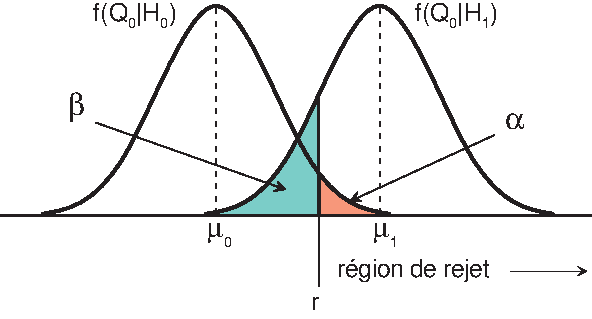
\includegraphics[width=11cm]{alpha_beta}$$
	\label{alphabeta}
	\caption{Risques $\alpha$ et $\beta$}
\end{figure}

\begin{figure}[ht]
	$$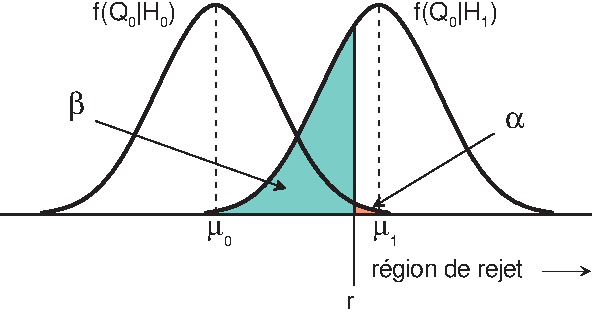
\includegraphics[width=11cm]{alpha_beta_2}$$
	\caption{$\alpha$ petit, donc $\beta$ grand}
\end{figure}


\begin{figure}[ht]
	$$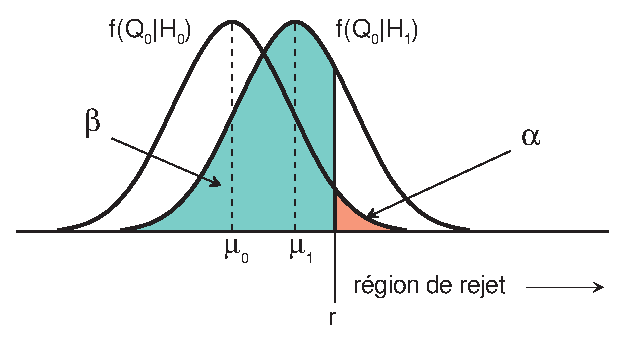
\includegraphics[width=11cm]{alpha_beta_3}$$
	\caption{$H_1$ peu diff�rent de $H_0$ $\Rightarrow \beta$ grand}
\end{figure}


\begin{defi}
Le \emph{risque total d'erreur} est d�fini par la relation
$$\alpha \;\underbrace{P(H_0)}_{\text{inconnu}}\;+\;\beta \;\underbrace{P(H_1)}_{\text{inconnu}}$$
\end{defi}

Cette relation implique que le risque total est inconnu.\\
En pratique, on d�termine le seuil critique $r$ pour un $\alpha$ choisi arbitrairement petit (en g�n�ral $5\;\%$ ou $10\;\%$).

\subsection{Proc�dure de test statistique}
Pour tester une hypoth�se, vous pouvez proc�der ainsi:
\begin{enumerate}
	\item Sp�cifier la valeur de la population d'int�r�t.
	\item Formuler l'hypoth�se nulle $H_0$ et l'hypoth�se alternative $H_1$
	\item Choisir le niveau de signification $\alpha$
	\item D�terminer la r�gion critique.
	\item Calculer la statistique associ�e � l'�chantillon.
	\item Rejeter $H_0$ si la statistique appartient � la r�gion critique.\\
	Ne pas rejeter $H_0$ dans le cas contraire.
	\item �noncer une conclusion.
\end{enumerate}

%%%%%%%%%%%%%%%%%%%%%%%%%%%%%%%%%%%%%%%%%%%%%%%
%%                                           %%
%% Test mu, sigma connu, grand �chantillon   %%
%%                                           %%
%%%%%%%%%%%%%%%%%%%%%%%%%%%%%%%%%%%%%%%%%%%%%%%
\section{Test de $\mu$, $\sigma^2$ connu, grand �chantillon}
Lorsque nous connaissons la variance et que l'�chantillon est de grande taille $n\geq 30$, nous savons par le th�or�me central limite \ref{theoCentralLimit} que l'estimateur de la moyenne $\bar{x}$ suit une loi normale de moyenne $\mu$ et d'�cart type $\frac{\sigma}{\sqrt{n}}$. La statistique � utiliser est donc

$$z=\frac{\bar{x}-\mu}{\frac{\sigma}{\sqrt{n}}}$$
o�\\
\begin{tabular}{cl}
	$\bar{x}$ & = moyenne de l'�chantillon\\
	$\mu$     & = moyenne suppos�e de la population �tudi�e\\
	$\sigma$  & = �cart type de la population\\
	$n$       & = taille de l'�chantillon
\end{tabular}

\begin{ex}
\label{ex:testMuSigmaConnu}
Une �tude sur la mobilit� des employ�s de l'entreprise ''Jeux Mendors'' affirme que la moyenne des temps de trajet des employ�s pour venir � leur travail exc�de 40 minutes. Vous devez tester cette affirmation avec une niveau de signification de 0.05. Pour cela, 100 employ�s vous ont indiqu� leur temps de trajet actuel, dont la moyenne est 43.5 minutes. Bas� sur une �tude pr�c�dente, vous pouvez supposer que l'�cart type de la population est de 8 minutes.

\begin{enumerate}
	\item La valeur de la population d'int�r�t est le temps de trajet.
	\item Les hypoth�ses nulle et alternative sont:\\
	  \begin{tabular}{cl}
	  $H_0$ & $\mu\leq 40$ minutes\\
	  $H_1$ & $\mu >40$ minutes\\	
    \end{tabular}
  \item Le niveau de signification est de 0.05
  \item La r�gion critique est $[z_{0.05}=1.645;\infty[$
  \item La statistique est $z=\frac{43.5-40}{\frac{8}{\sqrt{100}}}=4.38$
  \item Comme 4.38 appartient � la r�gion critique, l'hypoth�se $H_0$ est rejet�e.
  \item La conclusion est que la moyenne des temps de trajet exc�de 40 minutes.
\end{enumerate}
\end{ex}


%%%%%%%%%%%%%
\newpage
%%%%%%%%%%%%%
%%%%%%%%%%%%%%%%%%%%%%%%%%%%%%%%%%%%%%%%%%%%%%%
%%                                           %%
%% Test mu, sigma inconnu, grand �chantillon %%
%%                                           %%
%%%%%%%%%%%%%%%%%%%%%%%%%%%%%%%%%%%%%%%%%%%%%%%
\section{Test de $\mu$, $\sigma^2$ inconnu, grand �chantillon}
Dans la plupart des cas pratiques, la variance de la population n'est pas connue. Toutefois, il est possible d'estimer cette variance de la population � l'aide de la variance de l'�chantillon. Si la taille de l'�chantillon est suffisamment grande, en pratique d'au moins 30, la statistique de test peut �tre approch�e par une $z$-valeur gr�ce au th�or�me central limite \ref{theoCentralLimit}.

$$z=\frac{\bar{x}-\mu}{\frac{s}{\sqrt{n}}}$$
o�\\
\begin{tabular}{cl}
	$\bar{x}$ & = moyenne de l'�chantillon\\
	$\mu$     & = moyenne suppos�e de la population �tudi�e\\
	$s$       & = �cart type de l'�chantillon\\
	$n$       & = taille de l'�chantillon
\end{tabular}

%%%%%%%%%%%%%%%%%%%%%%%%%%%%%%%%%%%%%%%%%%%%%%%
%%                                           %%
%% Test mu, sigma inconnu, petit �chantillon %%
%%                                           %%
%%%%%%%%%%%%%%%%%%%%%%%%%%%%%%%%%%%%%%%%%%%%%%%
\section{Test de $\mu$, $\sigma^2$ inconnu, petit �chantillon}\label{sec:mu-sigmainconnu-petit}
Lorsque la variance de la population n'est pas connue et que l'on ne dispose que d'un �chantillon de petite taille $n<30$, nous pouvons utiliser la distribution de Student dans le test de la moyenne.

La statistique de test � utiliser suit une loi de Student � $n-1$ degr�s de libert�s:
$$t=\frac{\bar{x}-\mu}{\frac{s}{\sqrt{n}}}$$
o�\\
\begin{tabular}{cl}
	$\bar{x}$ & = moyenne de l'�chantillon\\
	$\mu$     & = moyenne suppos�e de la population �tudi�e\\
	$s$       & = �cart type de l'�chantillon\\
	$n$       & = taille de l'�chantillon
\end{tabular}

Toutefois, afin de pouvoir utiliser la $t$-distribution (= distribution de Student), nous devons faire la \textcolor{red}{supposition suivante}:\\
\textsc{La population est normalement distribu�e}

\begin{ex}\label{exMuSigmaInconnuPetit}
Nous voulons tester la moyenne d'un �chantillon du nombre d'employ�s par petite entreprise suisse contre la moyenne de la population, $\mu=35$, en ne connaissant pas la valeur de la variance de la population. Par des �tudes pr�c�dentes, nous savons que le nombre d'employ�s est distribu� selon une loi normale. Pour cela, 20 petites entreprises suisses ont �t� interrog�es sur le nombre d'employ�s qu'elles occupent. La moyenne calcul�e vaut $\overline{x}=27$ et la variance calcul�e vaut $s^2=334.7$. Nous souhaitons un niveau de signification de 0.05.

\begin{enumerate}
	\item La valeur de la population d'int�r�t est le nombre d'employ�s de petites entreprises suisses.
	\item Les hypoth�ses nulle et alternative sont:\\
	  \begin{tabular}{cl}
	  $H_0$ & $\mu = 35$ personnes\\
	  $H_1$ & $\mu \not= 35$ personnes\\	
    \end{tabular}
  \item Le niveau de signification est de 0.05
  \item La r�gion critique est compos�e de 2 zones distinctes car nous avons un test bilat�ral � effectuer.\\
		$$R = R_1 \cup R_2 = \{t_0 \mid t_0 \leq r_1\} \cup \{t_0 \mid t_0 \geq r_2\}$$
    \begin{center}
    \setlength{\unitlength}{1cm}
    \begin{picture}(5,2)
        \thicklines
        \put(-0.2,1.3){\line(1,0){5.4}}
        \put(.9,1.5){\line(-1,-2){.2}}
        \put(.6,1.5){\line(-1,-2){.2}}
        \put(.3,1.5){\line(-1,-2){.2}}
        \put(.0,1.5){\line(-1,-2){.2}}
        \put(1,1.1){\parbox[t]{0em}{\makebox[0pt][c]{]}}}
        \put(1,0.4){\parbox[t]{0em}{\makebox[0pt][c]{$r_1$}}}
        \put(4.1,1.1){\line(1,2){.2}}
        \put(4.4,1.1){\line(1,2){.2}}
        \put(4.7,1.1){\line(1,2){.2}}
        \put(5,1.1){\line(1,2){.2}}
        \put(4,1.1){\parbox[t]{0em}{\makebox[0pt][c]{[}}}
        \put(4,0.4){\parbox[t]{0em}{\makebox[0pt][c]{$r_2$}}}
        \put(2.6,1.8){\parbox[t]{0em}{\makebox[0pt][c]{$A$}}}
        \put(.3,1.8){\parbox[t]{0em}{\makebox[0pt][c]{$R_1$}}}
        \put(4.8,1.8){\parbox[t]{0em}{\makebox[0pt][c]{$R_2$}}}
    \end{picture}
    \end{center}

    Les seuils critiques $r_1$ et $r_2$ sont d�termin�s � partir de la table de la loi de Student:\\
		$P(T_0 \geq r_2) = \frac{\alpha}{2} = 0.025$ et donc $r_2=t_{\alpha/2,19}= 2.093$\\
    Donc $r_1=-t_{\alpha/2,19}= - 2.093$
  \item La statistique est
  $$t = \frac{27 - 35}{\sqrt{\frac{334.7}{20}}} = -1.955587$$
  \item Comme $t=-1.955587$ n'appartient pas � la r�gion critique, l'hypoth�se $H_0$ n'est pas rejet�e.
  \item La conclusion est que la vraie moyenne de la population peut �tre �gale � 35 employ�s par petite entreprise suisse.
\end{enumerate}
\end{ex}

%%%%%%%%%%%%%%%%%%%%%%%%%%%%%%%%%%%%%%%%%%%%%%%
%%                                           %%
%%        Value at Risk                      %%
%%                                           %%
%%%%%%%%%%%%%%%%%%%%%%%%%%%%%%%%%%%%%%%%%%%%%%%
\section{Value at Risk}
Nous traitons ici tr�s sommairement d'une mesure de risque tr�s utilis�e en finance. Le but n'est pas d'expliciter de mani�re exhaustive tout ce que le concept de Value at Risk (VaR) recouvre, mais simplement de donner un exemple d'application de test unilat�ral sur la moyenne. Nous allons voir comment est calcul�e une VaR param�trique par l'approche delta-normale.

\begin{defi}
La \emph{Value at Risk} est d�finie comme la perte maximale sur un horizon donn� $T$, avec un niveau de confiance $1-\alpha$.
\end{defi}

De mani�re statistique, en consid�rant une variable al�atoire $X$ suivant une loi normale $\norm(\mu,\sigma^2)$, la VaR s'exprime comme
$$P\left( X\leq \mbox{VaR}(\alpha,T)\right) = \alpha \quad\Leftrightarrow\quad P\left( X\geq \mbox{VaR}(\alpha,T)\right) = 1-\alpha$$

La notion de risque financier peut �tre estim�e � l'aide de l'�cart type annuel des performances financi�res, appel� dans le jargon bancaire la \emph{volatilit�}. L'horizon est quant � lui souvent donn� en jours (1, 10, ...), qui est � mettre en regard du nombre de jours ouvrables consid�r� dans la branche (250 ou 252 g�n�ralement). Consid�rons $X$ une variable al�atoire indiquant les rendements, suivant une m�me loi normale $\norm(\mu,\sigma^2)$ sur une seule p�riode.  Alors, sur la p�riode $T$, les rendements sont �galement gausssiens de moyenne $\mu T$ et de variance $\sigma^2 T$. La variable centr�e r�duite s'�crit :
$$z_{\alpha}=\frac{\mbox{VaR}(\alpha,T)-\mu T}{\sigma\sqrt{T}}$$
Et donc
$$\mbox{VaR}(\alpha,T) = \mu T + z_{\alpha}\sigma\sqrt{T}$$

\begin{ex}
{\it\small Source: Rapport annuel 2007 de l'UBS}\\
La position du secteur Banque d'investissement de l'UBS, sur un horizon de 1 jour, � un niveau de confiance de 99\%, en utilisant des donn�es sur 5 ans, est de
\begin{itemize}
	\item 149 millions en 2007
	\item 160 millions en 2006
\end{itemize}
\end{ex}


%%%%%%%%%%%%%%%%%%%%%%%%%%%%%%%%%%%%%%%%%%%%%%%
%%                                           %%
%%        Test de la proportion              %%
%%                                           %%
%%%%%%%%%%%%%%%%%%%%%%%%%%%%%%%%%%%%%%%%%%%%%%%
\section{Test de la proportion}
Il est souvent utile de pouvoir contr�ler l'�volution d'une proportion. Par exemple, un responsable qualit� doit s'assurer qu'une machine de production reste bien calibr�e et satisfait ainsi aux normes �tablies pour cette machine. Comme une proportion peut �tre consid�r�e comme une moyenne particuli�re, les m�mes concepts peuvent �tre appliqu�s dans le cas d'une proportion.

La statistique de test � utiliser, suivant une loi normale, est:
$$z=\frac{\bar{p}-\pi}{\sqrt{\frac{\pi(1-\pi)}{n}}}$$
o�\\
\begin{tabular}{cl}
	$\bar{p}$ & = proportion de l'�chantillon\\
	$\pi$       & = proportion suppos�e de la population �tudi�e\\
	$n$       & = taille de l'�chantillon
\end{tabular}

Toutefois, afin de pouvoir utiliser la distribution normale, nous devons faire la \textcolor{red}{supposition suivante}:\\
\textsc{La taille de l'�chantillon doit �tre suffisamment grande}\\
en pratique, il suffit que
$$n\bar{p}\geq 5\quad\mbox{et}\quad n(1-\bar{p})\geq 5$$

\begin{ex}\label{exTestProportion}
Un contr�le interne doit �tre effectu� dans une banque pour v�rifier que les contrats des hypoth�ques accord�es comportent tous les documents n�cessaires. Parfois, un contrat ne comporte pas tous les documents, auquel cas, le dossier n'est pas complet. La banque a octroy� 22500 hypoth�ques. et exige qu'il n'y ait pas plus d'1\% de contrats incomplets. L'�quipe charg�e du contr�le n'a pas le temps d'examiner les 22500 contrats et d�cide de contr�ler 600 contrats choisis al�atoirement, et fixe le niveau de signification � 0.02. Elle trouve 9 contrats incomplets.
\begin{enumerate}
	\item La valeur de la population d'int�r�t est la proportion de contrats incomplets
	$$\pi=0.01$$
	Comme la taille de l'�chantillon est suffisamment grande:\\
	$$600\times 0.01 = 6\geq 5\quad\mbox{et}\quad 600\times (1-0.01)=594\geq 5$$
	l'utilisation de la statistique $z$ est possible.
	\item $H_0$: $\pi\leq 0.01$\\
	      $H_1$: $\pi> 0.01$
	\item Le niveau de signification est $\alpha = 0.02$
	\item La r�gion critique est $[z_\alpha \approx 2.05;\infty [$
	\item La statistique associ�e � l'�chantillon est
	$$\bar{p}=9/600=0.015 \quad z=\frac{0.015-0.01}{\sqrt{\frac{0.01(1-0.01)}{600}}}=1.23$$
	\item Comme $z=1.23<2.05$, $H_0$ n'est pas rejet�e.
	\item L'�quipe de contr�le interne peut donc supposer que l'exigence de la banque est satisfaite.
\end{enumerate}
\end{ex}

\begin{rem}
\begin{itemize}
	\item Lors d'un test unilat�ral, la valeur critique est d�termin�e par 
	\begin{itemize}
		\item $z_{\alpha}$ s'il s'agit d'un test unilat�ral � droite
		\item $-z_{\alpha}$ s'il s'agit d'un test unilat�ral � gauche
	\end{itemize}
	\item Lors d'un test bilat�ral, les valeurs critiques sont d�termin�es par $\pm z_{\alpha/2}$
\end{itemize}
\end{rem}

%%%%%%%%%%%%%%%%%%%%%%%%%%%%%%%%%%%%%%%%%%%%%%%
%%                                           %%
%%     Test de la variance, mu inconnu       %%
%%                                           %%
%%%%%%%%%%%%%%%%%%%%%%%%%%%%%%%%%%%%%%%%%%%%%%%
\section{Test de la variance avec moyenne inconnue}
Lorsque l'int�r�t se porte sur la dispersion des donn�es, l'indicateur utilis� le plus souvent est l'�cart type. Or, il n'existe pas de test sur l'�cart type, mais par contre, des tests existent sur la variance. Comme g�n�ralement la moyenne de la population n'est pas connue, afin de calculer la variance, il faudra aussi l'estimer gr�ce � l'�chantillon.

La statistique de test � utiliser suit une loi du $\ki^2$ � $n-1$ degr�s de libert�s:
$$\ki^2=\frac{(n-1)s^2}{\sigma^2}$$
o�\\
\begin{tabular}{cl}
	$\sigma^2$ & = variance suppos�e de la population\\
	$s^2$       & = variance de l'�chantillon\\
	$n$       & = taille de l'�chantillon
\end{tabular}

Hypoth�se: �chantilllon provenant d'une population dont les �l�ments sont \textcolor{red} {ind�pendants et identiquement distribu�s, de distribution normale}.

\begin{rem}
Le nombre de degr�s de libert� n'est pas $n$ mais $n-1$ car la v�ritable moyenne  (de la population) n'est pas connue. Il faut donc l'estimer par la moyenne de l'�chantillon.
\end{rem}

\begin{ex}
Le syst�me de satellites Galileo est un projet europ�en pr�vu pour concurrencer le syst�me GPS am�ricain actuel. Supposons qu'un constructeur de GPS fournisse un appareil utilisant Galileo, et annonce une pr�cision de $\pm 5$ cm. Un test est effectu� pour v�rifier cette affirmation, en utilisant un �chantillon de taille 20, et un niveau de signification de 0.05. Les donn�es de l'�chantillon suivent une loi normale, et l'on peut supposer qu'il en est de m�me pour la population. La variance de l'�chantillon est calcul�e $s^2=0.0108$.

\begin{enumerate}
	\item La valeur de la population d'int�r�t est la pr�cision de l'appareil, qui est une variance.
	\item $H_0$: $\sigma^2\leq 0.0025$\\
	      $H_1$: $\sigma^2 > 0.0025$
	\item Le niveau de signification est fix� � $\alpha = 0.05$
	\item La r�gion de rejet du test est l'ensemble des valeurs sup�rieures �
	$$\ki^2_{0.05}\approx 30.1435$$
	La valeur limite calcul�e est celle pour une distribution $\ki^2$ � $20-1=19$ degr�s de libert�, et un niveau de signification de 0.05.
	\item La statistique associ�e � l'�chantillon est
	$$s^2=0.0108 \quad \ki^2=\frac{(20-1)0.0108}{0.0025}=82.08$$
	\item Comme  $\ki^2=82.08$ appartient � la r�gion critique, l'hypoth�se $H_0$ est rejet�e.
	\item Il est donc tr�s peu probable que la pr�cision  annonc�e soit correcte.
\end{enumerate}
\end{ex}

%%%%%%%%%%%%%%%%%%%%%%%%%%%%%%%%%%%%%%%%%%%%%%%
%%                                           %%
%% M�thode de la p-valeur                    %%
%%                                           %%
%%%%%%%%%%%%%%%%%%%%%%%%%%%%%%%%%%%%%%%%%%%%%%%
\section{M�thode de la $p$-valeur}
Il existe une autre m�thode permettant d'interpr�ter le r�sultat de n'importe quel test d'hypoth�se selon la m�me proc�dure. Cette proc�dure, dite de la $p$-valeur, est notamment utilis�e lorsque l'on travaille avec un ordinateur.

\begin{defi}
La \emph{$p$-valeur}, appel�e \emph{niveau (ou degr�) de signification observ�},  est la probabilit� d'observer l'�chantillon r�ellement utilis� sachant que l'hypoth�se nulle $H_0$ est vraie.
\end{defi}

La $p$-valeur s'interpr�te aussi comme la probabilit� d'obtenir � partir d'un autre �chantillon tir� de la m�me population une valeur du param�tre test� au moins aussi extr�me (plus �loign�e de $H_0$) que la valeur r�ellement observ�e.

Voici comment interpr�ter cette $p$-valeur:\\
Si la $p$-valeur calcul�e est plus petite que la probabilit� $\alpha$ associ�e � la r�gion de rejet, alors l'hypoth�se nulle $H_0$ est rejet�e. Sinon, l'hypoth�se nulle $H_0$ n'est pas rejet�e. Cette m�thode est populaire car la plupart des logiciels, y-compris Excel, Calc, Gnumeric, ...,  permettent de calculer cet $p$-valeur. L'avantage de rapporter cette $p$-valeur est qu'elle donne plus d'information que simplement le rejet ou non d'une hypoth�se. En effet, elle donne le degr� de signification associ� au r�sultat.

\begin{ex}
Dans le cas d'un test unilat�ral � gauche, la situation d�crite par le graphique suivant conduit au rejet de $H_0$, car la $p$-valeur (zone hachur�e verticalement) est plus petite que le risque $\alpha$ (zone hachur�e horizontalement).

 \begin{center}
 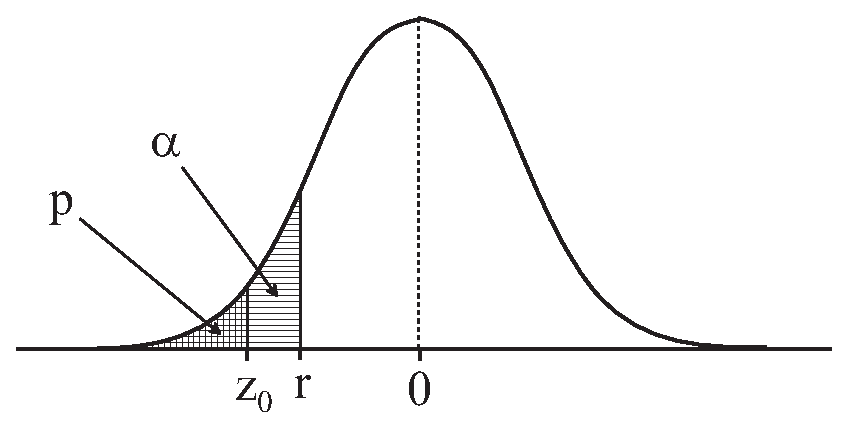
\includegraphics[width=11cm]{p_value_4}
 \end{center}
\end{ex}

\newpage
\subsection{Proc�dure de test statistique utilisant la $p$-valeur}
Pour tester une hypoth�se en utilisant la $p$-valeur, vous pouvez proc�der ainsi:
\begin{enumerate}
	\item Sp�cifier la valeur de la population d'int�r�t.
	\item Formuler l'hypoth�se nulle $H_0$ et l'hypoth�se alternative $H_1$
	\item Choisir le niveau de signification $\alpha$
	\item D�terminer la r�gion critique:\\
	Si la $p$-valeur est inf�rieure � $\alpha$, alors rejeter $H_0$\\
	Sinon, ne pas rejeter $H_0$
	\item Calculer la $p$-valeur associ�e � l'�chantillon.
	\item Prendre une  d�cision.\\
	(Rejeter $H_0$ seulement si la $p$-valeur est inf�rieure � $\alpha$)
	\item �noncer une conclusion.
\end{enumerate}

\begin{ex}
Test unilat�ral\\
Reprenons l'exemple \ref{ex:testMuSigmaConnu}.\\
Une �tude sur la mobilit� des employ�s de l'entreprise ''Jeux Mendors'' affirme que la moyenne des temps de trajet des employ�s pour venir � leur travail exc�de 40 minutes. Vous devez tester cette affirmation avec une niveau de signification de 0.05. Pour cela, 100 employ�s vous ont indiqu� leur temps de trajet actuel, dont la moyenne est 43.5 minutes. Bas� sur une �tude pr�c�dente, vous pouvez supposer que l'�cart type de la population est de 8 minutes.

\begin{enumerate}
	\item La valeur de la population d'int�r�t est le temps de trajet moyen.
	\item Les hypoth�ses nulle et alternative sont:\\
	  \begin{tabular}{cl}
	  $H_0$ & $\mu\leq 40$ minutes\\
	  $H_1$ & $\mu >40$ minutes\\	
    \end{tabular}
  \item Le niveau de signification est de 0.05
  \item La r�gion critique est celle dont la $p$-valeur est inf�rieure � $\alpha$
  \item Le calcul de la $p$-valeur s'effectue de la mani�re suivante:
  $$z=\frac{43.5-40}{\frac{8}{\sqrt{100}}}=4.38$$
  Il faut ensuite calculer la probabilit� suivante:
  $$p\mbox{-valeur} = \mbox{P}(z>4.38)=1-\mbox{P}(z\leq 4.38) \approx 0$$
  \item Comme la $p$-valeur appartient � la r�gion critique, l'hypoth�se $H_0$ est rejet�e.
  \item La conclusion est que la moyenne des temps de trajet exc�de 40 minutes.
\end{enumerate}
\end{ex}

Lors d'un test bilat�ral, on ne peut se trouver que dans l'une ou l'autre r�gion de rejet du test, et non pas dans les deux � la fois. Consid�rons une statistique suivant une distribution sym�trique. Afin de calculer la $p$-valeur, on commence par calculer la probabilit� que la statistique prenne des valeurs plus extr�mes que celles obtenue � partir de l'�chantillon, du c�t� correspondant � la situation observ�e. Puis, cette probabilit� est doubl�e pour obtenir la $p$-valeur.

\begin{ex}
\label{ex:moyennePME}
Test bilat�ral\\
Reprenons l'exemple \ref{exMuSigmaInconnuPetit}\\
Nous voulons tester la moyenne d'un �chantillon du nombre d'employ�s par petite entreprise suisse contre la moyenne de la population, $\mu=35$, en ne connaissant pas la valeur de la variance de la population. Par des �tudes pr�c�dentes, nous savons que le nombre d'employ�s est distribu� selon une loi normale. Pour cela, 20 petites entreprises suisses ont �t� interrog�es sur le nombre d'employ�s qu'elles occupent. La moyenne calcul�e vaut $\overline{x}=27$ et la variance calcul�e vaut $s^2=334.7$. Nous souhaitons un niveau de signification de 0.05.

\begin{enumerate}
	\item La valeur de la population d'int�r�t est le nombre moyen d'employ�s de petites entreprises suisses.
	\item Les hypoth�ses nulle et alternative sont:\\
	  \begin{tabular}{cl}
	  $H_0$ & $\mu = 35$ employ�s\\
	  $H_1$ & $\mu \not= 35$ employ�s\\	
    \end{tabular}
  \item Le niveau de signification est de 0.05
  \item La r�gion critique est celle dont la $p$-valeur est inf�rieure � $\alpha$
  \item Le calcul de la $p$-valeur s'effectue de la mani�re suivante:
  $$t = \frac{27 - 35}{\sqrt{\frac{334.7}{20}}}= -1.955587$$
  Comme la moyenne de l'�chantillon est inf�rieure � la moyenne de la population postul�e sous $H_0$, on consid�re tout d'abord la r�gion de rejet de gauche.
  Il faut donc calculer la probabilit� suivante:
  $$\mbox{P}(t_{\frac{\alpha}{2},19}<-1.955587)\approx 0.0327$$
  S'agissant d'un test bilat�ral, cette probabilit� doit �tre doubl�e\\
  $p$-value = $2\times \mbox{P}(\frac{\alpha}{2},19<-1.955587)\approx 0.0654$
  \item Comme la $p$-valeur n'appartient pas � la r�gion critique, l'hypoth�se $H_0$ n'est pas rejet�e.
  \item La conclusion est que la vraie moyenne de la population peut �tre �gale � 35 employ�s par petite entreprise suisse.
\end{enumerate}
\end{ex}

\newpage
%%%%%%%%%%%%%%%%%%%%%%%%%%%%%%%%%%%%%%%%%%%%%%%
%%                                           %%
%%  Relation IC et tests statistiques        %%
%%                                           %%
%%%%%%%%%%%%%%%%%%%%%%%%%%%%%%%%%%%%%%%%%%%%%%%
\section{Relation entre IC et tests statistiques}
\subsection{Test dans l'unit� du param�tre}
Dans l'exemple pr�c�dent \ref{ex:moyennePME}, nous avons transform� la valeur observ�e $\overline{x}=27$ en une valeur sans unit� $t_0=-1.955587$ pouvant �tre compar�e avec les seuils de la loi de Student, en conservant un niveau de signification $\alpha=0.05$. De fa�on �quivalente, il est �galement possible d'effectuer le
test en comparant la valeur observ�e $\overline{x}=27$ avec des transformations $r_{1, \bar x}$ et $r_{2, \bar x}$ des seuils de la loi
de Student.
$$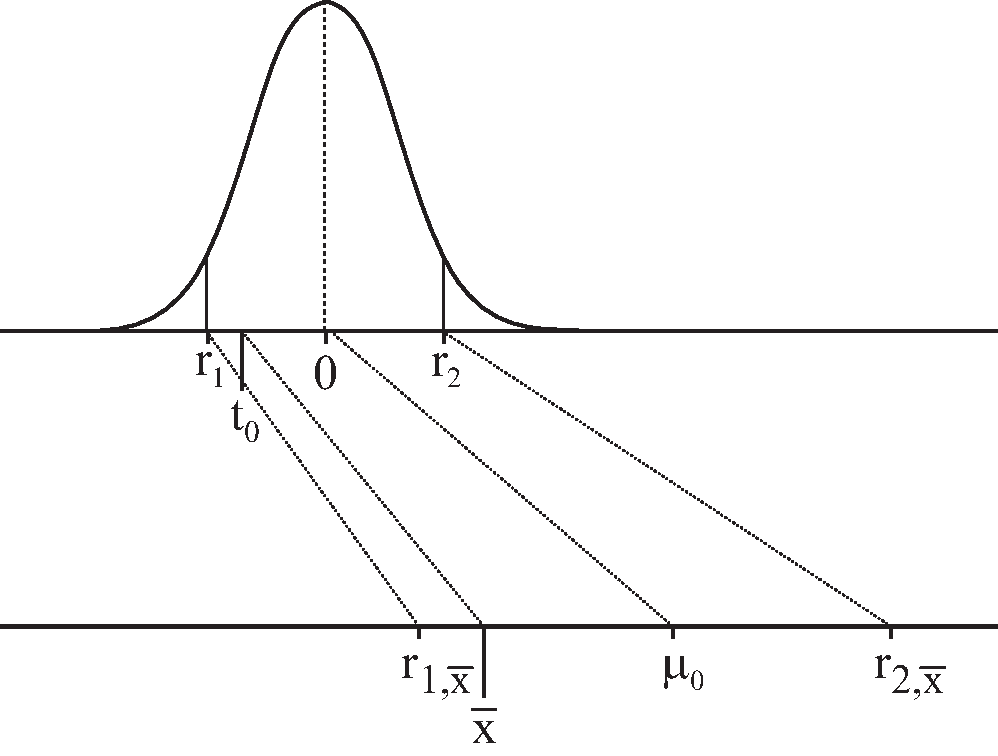
\includegraphics[width=12cm]{test_t_vs_x}$$
\'Etant donn� que nous avons utilis� la statistique
$$t = \frac{\bar{x} - \mu}{\hat\sigma_{\bar{x}}}$$
nous pouvons effectuer la transformation suivante
$$\bar{x} = \mu + t \; \hat\sigma_{\bar{x}}$$
et les seuils de rejet dans l'unit� de mesure de l'�chantillon s'�crivent
\begin{eqnarray*}
    r_{1,\bar{x}} &=& \mu + t_{1-\frac{\alpha}{2},19} \;
\hat{\sigma}_{\bar x}\\
 &\approx& 35 - 2.093024 \cdot 4.090843 \approx 26.43777
\end{eqnarray*}
et
\begin{eqnarray*}
    r_{2,\bar{x}} &=& \mu + t_{\frac{\alpha}{2},19} \;
\hat{\sigma}_{\bar{x}}\\
 &\approx & 35 + 2.093024 \cdot 4.090843 \approx 43.56223
\end{eqnarray*}
Comme $\overline{x}=27$ se trouve entre les deux seuils, l'hypoth�se $H_0$ est accept�e.

\subsection{Intervalle de confiance et test statistique}
Reprenons encore l'exemple pr�c�dent avec variance inconnue et calculons un intervalle de confiance pour $\mu$ en gardant un risque
$\alpha=0.05$.
    \begin{eqnarray*}
        \mu & \in & \bar{x} \pm \hat\sigma_{\bar{x}}\;t_{\frac{\alpha}{2},n-1}\\
         & \approx & 27 \pm 4.09 \cdot 2.093 \\
            & = & 27 \pm 8.56
    \end{eqnarray*}
Et donc  P($\mu \in [18.44 , 35.56]$) = 95\%

La largeur de l'intervalle de confiance construit autour de $\overline{x}$ est identique � la distance s�parant les deux seuils de rejet du test.
$$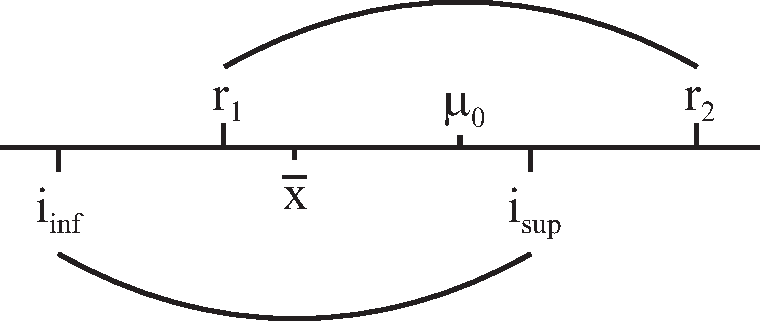
\includegraphics[width=10cm]{test_vs_interval}$$
Nous pouvons d�duire de la figure ci-dessus que lorsque le test bilat�ral est accept�,
$$r_1 < \overline{x} < r_2$$
ce qui implique
$$i_{\inf} < \mu_0 < i_{\sup}$$
Il y a donc �quivalence entre le test d'hypoth�se bilat�ral et l'intervalle de confiance:\\
Si $\mu_0$ se trouve dans l'intervalle de confiance construit autour de $\overline{x}$, alors l'hypoth�se $H_0: \mu=\mu_0$ est accept�e et vice versa.

\newpage
%%%%%%%%%%%%%%%%%%%%%%%%%%%%%%%%%%%%%%%%%%%%%%%
%%                                           %%
%%                R�sum�                     %%
%%                                           %%
%%%%%%%%%%%%%%%%%%%%%%%%%%%%%%%%%%%%%%%%%%%%%%%
\section{R�sum�}
Le tableau suivant r�sume les distributions utilis�es pour repr�senter la moyenne, la proportion et la variance d'une population.

\begin{center}
    \begin{tabular}{|c|l|c|}
    \hline&&\\[-1.5ex]
    estim�  & hypoth�se    & distribution
    \\[.5ex]
    \hline&&\\[-1ex]
    $\mu$   & $\sigma^2$ connu,  &\\
            & distr. normale ou $n\geq 30$
        & $Z =
%    \dfrac{\bar X-\mu}{\sigma/\sqrt{n}}=  \dfrac{\bar X-\mu}{\sigma_{\bar X}}\;\sim\norm (0,1)$
    \dfrac{\bar X-\mu}{\sigma/\sqrt{n}}\sim\norm (0,1)$
    \\[3ex]
  & $\sigma^2$ inconnu, distr. normale
     & $T_{(n-1)} =
%    \dfrac{\bar X - \mu}{s/\sqrt{n-1}}=\dfrac{\bar X - \mu}{\hat \sigma_{\bar X}} \; \sim\st_{n-1}$
    \dfrac{\bar X - \mu}{s/\sqrt{n}}\sim\st_{n-1}$
    \\[3ex]
    \hline&&\\[-1ex]
    $\pi$ & $n\pi\geq 5$ et $n(1-\pi)\geq 5$ &
    $Z=\frac{\bar{P}-\pi}{\sqrt{\frac{\pi(1-\pi)}{n}}}\sim\norm (0,1)$
    \\[3ex]
    \hline&&\\[-1ex]
    $\sigma^2$   & $\mu$ connu, distr. normale
    & $Q_{(n)}=\dfrac{\sum_{i=1}^{n} (X_i - \mu)^2}{\sigma^2} \;\sim\; \chi^2_n$
    \\[3ex]
     & $\mu$ inconnu, distr. normale
    & $Q_{(n-1)}=\dfrac{\sum_{i=1}^{n} (X_i - \bar X)^2}{\sigma^2}= \dfrac{(n-1)s^2}{\sigma^2} \;\sim\; \chi^2_{n-1}$
    \\[3ex]
    \hline
    \end{tabular}
\end{center}













\chapter{Tests non param�triques}
Lorsque nous voulons tester des hypoth�ses, nous devons tenir compte des conditions sous lesquelles les tests peuvent �tre faits. Par exemple, si nous d�sirons tester si la moyenne d'une population s'�carte significativement d'une valeur donn�e, et que sa distribution ne suit pas une loi normale, nous ne pouvons pas utiliser le test de la moyenne d�crit en \ref{sec:mu-sigmainconnu-petit}. Beaucoup de populations, comme par exemple le revenu moyen par famille, ont une distribution fortement asym�trique. Dans ce cas, l'emploi d'une proc�dure de test non param�trique est n�cessaire. Ces derni�res sont moins restrictives que les proc�dures de test param�trique.

Des tests du $\ki^2$ peuvent aussi se baser sur les diff�rences entre des effectifs th�oriques et des effectifs observ�s. Dans ce cas, ces tests ne comportent que tr�s peu de restrictions quant � la distribution sous-jacente, c'est pourquoi ils sont souvent class�s parmi les tests non param�triques.

%\section{Test des rangs sign�s de Wilcoxon}
%Ce test non param�trique n'est pas soumis � une restriction sur une forme particuli�re de distribution. Il est utilis� pour tester  la valeur hypoth�tique de la m�diane d'une population. Il se base sur le principe suivant:\\
%Puisque la m�diane s�pare une population en deux parties de m�me taille, la m�diane hypoth�tique de la population sera rejet�e si les donn�es se r�partissent trop fortement au-dessus ou au-dessous de cette valeur.
%
%\subsection{�chantillon de petite taille}
%La statistique de test $W$ suit la loi tabul�e pour le test des rangs sign�s de Wilcoxon en annexe \ref{sec:wilcoxonsigne}.
%\begin{enumerate}
%	\item Calculer les diff�rences $d_i$ entre chaque valeur et la m�diane postul�e $\tilde{\mu}$
%	\item Calculer la valeur absolue des diff�rences pr�c�dentes: $|d_i|$
%	\item D�terminer le rang pour chacune des valeurs $|d_i|$, en ne tenant pas compte des valeurs nulles.\\
%	Si des observations ont la m�me valeur $|d_i|$, alors affecter le rang moyen de ces observations.
%	\item Calculer la statistique $W$ qui est la somme des rangs dont les $d_i$ sont positifs.
%\end{enumerate}
%L'hypoth�se nulle est rejet�e si la valeur de la statistique est sup�rieure � celle de la valeur critique sup�rieure associ�e (test unilat�ral � droite ou test bilat�ral), ou inf�rieure � la valeur critique inf�rieure associ�e  (test unilat�ral � gauche ou test bilat�ral).
%
%\begin{ex}
%% \cite{groebner2005} p. 671
%% % Avec R:
%%x <- c(36400, 38500, 27000, 35000, 29000, 40000, 52000, 34000, 38900, 41000)
%%wilcox.test(x, alternative = "greater", mu=35000, exact = FALSE)
%
%Une �tude a �t� faite sur les salaires en d�but de carri�re des dipl�m�s de l'�cole ''Jess Aitou'', afin de savoir si le salaire m�dian est sup�rieur � 35000 Euros, � un seuil $\alpha=0.05$. Les donn�es r�colt�es sont les salaires en euros:\\
%$$\begin{array}{c}
%36400\\
%38500\\
%27000\\
%35000\\
%29000\\
%40000\\
%52000\\
%34000\\
%38900\\
%41000
%\end{array}$$
%Nous pouvons utiliser le test des rangs sign�s de Wilcoxon afin de r�pondre � l'objet de l'�tude.
%
%\begin{enumerate}
%	\item La valeur de la population d'int�r�t est le salaire m�dian en d�but de carri�re.
%	\item Les hypoth�ses nulle et alternative sont:\\
%	  \begin{tabular}{cl}
%	  $H_0$ & $\tilde{\mu} \leq 35'000$ euros\\
%	  $H_1$ & $\tilde{\mu} > 35'000$ euros\\	
%    \end{tabular}
%  \item Le niveau de signification est de 0.05
%  \item
%	$$
%	\begin{array}{crcccc}
%	\mbox{Salaire}=x_i & d_i=x_i-\tilde{\mu} & |d_i| & \mbox{Rang} & R_+ & R_-\\
%	\hline
%	36400 & 1400  & 1400 & 2   & 2 & \\
%	38500 &  3500 & 3500 & 3   & 3 & \\
%	27000 & -8000 & 8000 & 8   &   & 8\\
%	35000 &     0 & 0    &     &   & \\
%	29000 & -6000 & 6000 & 6.5 &   & 6.5\\
%	40000 &  5000 & 5000 & 5   & 5 & \\
%	52000 & 17000 & 17000& 9   & 9 & \\
%	34000 & -1000 & 1000 & 1   &   & 1\\
%	38900 &  3900 & 3900 & 4   & 4 & \\
%	41000 &  6000 & 6000 & 6.5 & 6.5\\
%	\hline
%	      &       &      &      & W=29.5 & 15.5
%	\end{array}$$	
%	Soit $n$ le nombre de $d_i$ diff�rents de 0. Il y a donc $n=9$ rangs attribu�s.\\
%	La valeur critique du test est $W_{\alpha}=37$
%	\item La statistique est $W=29.5$
%  \item Comme $$W=29.5<37$$
%  l'hypoth�se $H_0$ ne peut pas �tre rejet�e.
%  \item Nous ne pouvons donc pas conclure que le salaire m�dian en d�but de carri�re d�passe 35000 euros.
%\end{enumerate}
%\end{ex}
%
%\subsection{�chantillon de grande taille}
%Lorsque la taille de l'�chantillon est suffisamment grande, en pratique, lorsque $n>20$, alors la statistique de test $W$ peut �tre approch�e par une distribution normale. La statistique de test est transform�e en une $z$-valeur, qui suit une loi normale centr�e r�duite.
%$$z=\frac{W-\frac{n(n+1)}{4}}{\sqrt{\frac{n(n+1)(2n+1)}{24}}}$$
%o�\\
%\begin{tabular}{cl}
%	$n$       & = taille de l'�chantillon\\
%	$W$ & = somme des rangs positifs $R_+$
%\end{tabular}

%\chapter{Test du $\ki^2$}
% Des tests du $ki^2$ peuvent aussi se baser sur les diff�rences entre des effectifs th�oriques et des effectifs observ�s. Dans ce cas, ces tests ne comportent que tr�s peu de restrictions quant � la distribution sous-jacente, c'est pourquoi ils sont souvent class�s parmi les tests non param�triques.

%%%%%%%%%%%%%%%%%%%%%%%%%%%%%%%%%%%%%%%%%%%%%%
%%                                          %%
%%     Test d'ajustement                    %%
%%                                          %%
%%%%%%%%%%%%%%%%%%%%%%%%%%%%%%%%%%%%%%%%%%%%%%
\section{Test d'ajustement}
Certains tests exigent que la distribution de la population suive une loi sp�cifique, comme la loi normale. Comment peut-on v�rifier que cette condition est satisfaite? Le test d'ajustement du $\ki^2$ permet justement de le faire. 
Le test d'ajustement du $\ki^2$ peut �tre utilis� pour d�terminer si un �chantillon provient d'une hypoth�tique distribution.

La proc�dure de test d�bute par l'acquisition d'un �chantillon de taille suffisamment grande. Les donn�es sont ensuite class�es en $k$ diff�rentes cat�gories, afin d'obtenir les fr�quences absolues observ�es $o_ij$, associ�es � chaque cat�gorie. En utilisant la distribution hypoth�tique, les fr�quences absolues th�oriques $e_ij$ sont calcul�es. Il suffit alors de comparer les fr�quences observ�es � celles th�oriques. Si une trop grande diff�rence existe, alors l'hypoth�se d'un �chantillon tir� de la distribution hypoth�tique est rejet�e.

La statistique � utiliser suit une loi du $\ki^2$ � $k-1$ degr�s de libert� et est calcul�e ainsi:
$$\ki^2=\sum\limits_{i=1}^k \frac{(o_i-e_i)^2}{e_i}$$
o�\\
\begin{tabular}{cl}
	$o_ij$ & = fr�quence observ�e pour la cat�gorie $i$\\
	$e_ij$     & = fr�quence th�orique pour la cat�gorie $i$\\
	$k$       & = nombre de cat�gories
\end{tabular}

Toutefois, afin de pouvoir utiliser ce test, nous devons faire la \textcolor{red}{supposition suivante}:\\
\textsc{La taille de l'�chantillon est suffisamment grande}

En pratique, un �chantillon de taille au moins 30 est suffisant, pour autant que les fr�quences observ�es par cellule sont suffisamment �lev�es.

\begin{ex}
Un nouveau directeur d'un centre d'appels pour FAI constate que le personnel est r�duit de 20\% les mercredi, jeudi et dimanche. Son pr�d�cesseur avait proc�d� ainsi car le nombre d'appels �tait 20\% moins �lev� ces jours-l�. Afin de savoir si tel est toujours le cas, il fait relever le nombre d'appels sur 1 mois pour chaque jour de la semaine et obtient les donn�es agr�g�es suivantes:

\begin{center}
\begin{tabular}{c|ccccccc}
	Jours & Lu & Ma & Me & Je & Ve & Sa & Di\\
	\hline
	Nombre d'appels & 1000 & 1200& 900 & 1000 & 1200& 1100 & 800
\end{tabular}
\end{center}

Il souhaite savoir s'il y a effectivement une baisse de 20\% les mercredi, jeudi et dimanche, avec un niveau de signification de 0.05.

\begin{enumerate}
	\item Les hypoth�ses nulle et alternative sont:\\
	  \begin{tabular}{cl}
	  $H_0$ & La distribution des appels est identique les lu, ma, ve et sa,\\
	        & et 20\% moins �lev�e les me, je et di.\\
	  $H_1$ & La distribution des appels n'est pas celle d�crite en $H_0$\\	  
    \end{tabular}
  \item Le niveau de signification est de 0.05
  \item La valeur critique est celle d'une distribution du $\ki^2$ � 6 degr�s de libert�s.\\
  $$\ki^2_{0.05}=12.5916$$ 
  \item Le nombre total d'appels sur la p�riode observ�e est 7200
  \begin{center} 
		\begin{tabular}{c|ccccccc}
			Jours & Lu & Ma & Me & Je & Ve & Sa & Di\\
			\hline
			$o_i$ & 1000 & 1200& 900 & 1000 & 1200& 1100 & 800\\
			$e_i$ & 1125 & 1125 & 900 & 900 & 1125 & 1125 & 900
		\end{tabular}
		\end{center}
% Dans R
% x <- seq(1:7)
% Jours <- c("Lundi", "Mardi", "Mercredi", "Jeudi", "Vendredi", "Samedi", "Dimanche")
% observe <- c(1000,1200,900,1000,1200,1100,800)
% theorique <- c(1125,1125,900,900,1125,1125,900)
% A terminer
		La statistique est alors $$\ki^2 = 46.6$$
  \item Comme $46.6>12.5916$, l'hypoth�se $H_0$ est rejet�e.
  \item La conclusion est que la distribution du nombre d'appels n'est plus telle qu'indiqu�e par le pr�c�dent directeur.
\end{enumerate}
\end{ex}

%%%%%%%%%%%%%%%%%%%%%%%%%%%%%%%%%%%%%%%%%%%%%%
%%                                          %%
%%     Test d'ind�pendance                  %%
%%                                          %%
%%%%%%%%%%%%%%%%%%%%%%%%%%%%%%%%%%%%%%%%%%%%%%
\section{Test d'ind�pendance de deux variables cat�gorielles}
Afin de tester l'ind�pendance de deux variables de type cat�goriel, nous allons utiliser une table de contingence.
Nous comparons alors les fr�quences observ�es avec les fr�quences th�oriques en cas d'ind�pendance. Si une trop grande diff�rence existe, alors l'hypoth�se d'ind�pendance des variables est rejet�e.

Les fr�quences th�oriques sont calcul�es ainsi:
$$e_{ij} = \frac{ (\mbox{Total ligne }i)\cdot(\mbox{ Total colonne }j) }{ \mbox{Taille de l'�chantillon}}$$

La statistique � utiliser est celle du $\ki^2$ � dl = $(c-1)(r-1)$ degr�s de libert�
$$\ki^2=\sum\limits_{i=1}^r\sum\limits_{j=1}^c\frac{(o_{ij}-e_{ij})^2}{e_{ij}}$$
o�\\
\begin{tabular}{cl}
	$o_i$ & = fr�quence observ�e de la cellule $(i,j)$\\
	$e_i$     & = fr�quence th�orique de la cellule $(i,j)$\\
	$r$       & = nombre de lignes\\
	$c$       & = nombre de colonnes
\end{tabular}

Toutefois, afin de pouvoir utiliser ce test, nous devons faire la \textcolor{red}{supposition suivante}:\\
\textsc{La taille de l'�chantillon est suffisamment grande}\\
En pratique, l'effectif observ� par cellule doit �tre d'au moins 5 unit�s.

\begin{ex}
Une recherche est effectu�e afin de savoir si le nombre de sorties le week-end est ind�pendant des r�sultats aux examens, avec un niveau de signification de 0.05. La table de contingence suivante r�sume les donn�es r�colt�es:

\begin{center}
\begin{tabular}{r|cccc|c}
	& \multicolumn{4}{c}{R�sultat} & \\
	& Insuffisant & Acquis & Bien & Excellent & {\it\small Total}\\
	\hline
	Sortie WE   & & & & & \\
	Jamais      & 84 & 50 & 50 & 16 & 200\\
	Occasionnel & 82 & 64 & 34 & 20 & 200\\
	Fr�quent    & 34 & 36 & 16 & 14 & 100\\
	\hline
	{\it\small Total} & 200 & 150 & 100 & 50 & 500 
\end{tabular}
\end{center}


\begin{enumerate}
	\item Les hypoth�ses nulle et alternative sont:\\
	  \begin{tabular}{cl}
	  $H_0$ & Les sorties du week-end sont ind�pendantes des r�sultats aux examens.\\
	  $H_1$ & les sorties du week-end ne sont PAS ind�pendantes des r�sultats aux examens\\	  
    \end{tabular}
  \item Le niveau de signification est de 0.05
  \item La valeur critique est celle d'une distribution du $\ki^2$ � $(3-1)(4-1)=6$ degr�s de libert�s.\\
  $$\ki^2_{0.05}=12.5916$$ 
  \item Les fr�quences th�oriques de la table de contingence sont
  
\begin{center}
\begin{tabular}{r|cccc|c}
	& \multicolumn{4}{c}{R�sultat} & \\
	& Insuffisant & Acquis & Bien & Excellent & {\it\small Total}\\
	\hline
	Sortie WE   & & & & & \\
	Jamais      & 80 & 60 & 40 & 20 & 200\\
	Occasionnel & 80 & 60 & 40 & 20 & 200\\
	Fr�quent    & 40 & 30 & 20 & 10 & 100\\
	\hline
	{\it\small Total} & 200 & 150 & 100 & 50 & 500 
\end{tabular}
\end{center}
		La statistique est alors $$\ki^2 = 10.88$$
  \item Comme $10.88<12.5916$, l'hypoth�se $H_0$ ne peut pas �tre rejet�e.
  \item La conclusion est qu'il n'y a pas suffisamment d'�vidence pour conclure que les sorties du week-end et le r�sultat aux examens ne sont pas ind�pendants.\\
  ... et ceci n'est aucunement une incitation � faire la f�te le week-end!
\end{enumerate}

% Dans R
%\begin{verbatim}
%sorres <- matrix(c(84,50,50,16,82,64,34,20,34,36,16,14),ncol=4,byrow=TRUE)
%rownames(sorres)<-c("Jamais","Occasionnel","Fr�quent")
%colnames(sorres)<-c("Insuffisant","Acquis","Bien","Excellent")
%sorres <- as.table(sorres)
%chisq.test(sorres)
%\end{verbatim}

\end{ex}
\chapter{R�gression lin�aire simple}
\section{Rappel}
\begin{defi}
 	L'analyse statistique de la relation entre deux ou plusieurs variables s'appelle l'\emph{analyse de r�gression}. Si seulement deux variables sont �tudi�es, il s'agit d'une analyse de r�gression simple. Lorsque la relation entre deux variables est lin�aire, elle porte le nom de \emph{r�gression lin�aire simple}.
\end{defi}

\begin{defi}
Le \emph{mod�le de r�gression lin�aire simple} est d�fini par l'�quation suivante:
$$y=\beta_0 + \beta_1 x + \epsilon$$
avec\\
\begin{tabular}{ccl}
$y$ &=& variable d�pendante (ou variable expliqu�e)\\
$x$ &=& variable ind�pendante (ou variable explicative)\\
$\beta_0$ &=& constante de la droite de r�gression pour la population\\
$\beta_1$ &=& pente de la droite de r�gression pour la population\\
$\epsilon$ &=& terme d'erreur ou r�sidu.
\end{tabular}
\end{defi}

Le mod�le de r�gression lin�aire simple se base sur les postulats suivants:
\begin{enumerate}
	\item Les r�sidus $\epsilon$ sont ind�pendants et identiquement distribu�s, suivant une loi normale.
	\item Le mod�le de r�gression lin�aire est l�gitime.
\end{enumerate}
Ce mod�le est estim� par la m�thode des moindres carr�s: la somme des carr�s des r�sidus est minimis�e, ce qui permet d'obtenir l'�quation suivante:
$$\hat{y}=b_0+b_1x$$

avec\\
\begin{tabular}{ccl}
$\hat{y}$ &=& valeur estim�e de $y$\\
$x$ &=& valeur de la variable ind�pendante\\[2mm]
$b_1$ &=& $\displaystyle \frac{s_{xy}}{s_x^2} = \frac{\sum (x_i-\bar{x})(y_i-\bar{y})} {\sum(x_i-\bar{x})^2}$\\[4mm]
$b_0$ &=& $\bar{y}-b_1\bar{x}$
\end{tabular}

\begin{defi}
 	Le \emph{coefficient de corr�lation lin�aire} d'un �chantillon est la valeur
$$r_{xy} = \frac{s_{xy}}{s_x\;s_y}=
\frac{ \sum(x_i-\bar{x})(y_i-\bar{y}) }{ \sqrt{\sum(x_i-\bar{x})^2\sum(y_i-\bar{y})^2} }$$
\end{defi}

\begin{rem}
Lorsqu'il n'y a que deux variables (ou aucune ambig�it� possible), le coefficient de corr�lation lin�aire est simplement not� $r$
\end{rem}

\section{Validit� d'une corr�lation}
Une corr�lation lin�aire $r$ �tant le plus souvent calcul�e � partir d'un �chantillon, sa valeur est sujette � des erreur d'�chantillonnage. Ainsi, $r_{xy}$ n'est qu'une estimation de la v�ritable valeur du coefficient de corr�lation lin�aire $\rho$. Il faut donc utiliser un test sur l'existence ou non d'une corr�lation lin�aire:

\begin{eqnarray*}
	H_0 &:& \rho=0\\
	H_1 &:& \rho\not=0
\end{eqnarray*}

La statistique de test � consid�rer est la suivante:
$$t = \frac{r}{\sqrt{\frac{1-r^2}{n-2}}}\quad dl=n-2$$
avec\\
\begin{tabular}{ccl}
t &=& nombre d'�cart-type de $r$ depuis 0\\
$r$ &=& coefficient de corr�lation lin�aire\\
$n$ &=& taille de l'�chantillon
\end{tabular}
	
Notons que ce test de Student suppose que
\begin{enumerate}
	\item Les donn�es sont quantitatives.
	\item Les deux variables $x$ et $y$ suivent une distribution bivari�e normale (i.e. leur distribution conjointe suit une loi normale).
\end{enumerate}

\begin{ex}
%p. 508 \ref{Groebner2005}
Une entreprise souhaite analyser la relation entre la taille d'une annonce publicitaire, et le nombre d'appels re�us g�n�r�s par l'annonce. Elle veut savoir s'il existe une corr�lation lin�aire positive entre ces deux variables, au seuil 0.05. Pour cela, elle demande � ses clients d'indiquer quelle annonce leur ont fait conna�tre l'entreprise.
Le d�pouillement de l'enqu�te sur 10 annonces donne:\\[3mm]

%% Dans R
%taille <- c(9, 16, 25, 16, 20, 16, 20, 20, 16, 9); taille <- 10*taille;
%proportion <- c(0.13, 0.16, 0.21, 0.18, 0.18, 0.19, 0.15, 0.17, 0.13, 0.11)
%cor(taille, proportion)
%cor.test(taille, proportion, method = "pearson", alternative = "greater")
\begin{tabular}{l|*{10}{r}}
Num annonce & 1 & 2 & 3 & 4 & 5 & 6 & 7 & 8 & 9 & 10\\
\hline
Taille [cm carr�s] & 90 & 160 & 250 & 160 & 200 & 160 & 200 & 200 & 160 & 90\\
\hline
Prop. d'appels & 0.13 & 0.16 & 0.21 & 0.18 & 0.18 & 0.19 & 0.15 & 0.17 & 0.13 & 0.11
\end{tabular}

\begin{enumerate}
	\item Le param�tre d'int�r�t est la corr�lation lin�aire $\rho$ entre la taille d'une annonce publicitaire et la proportion d'appels g�n�r�s par l'annonce. 
	\item Les hypoth�ses nulle et alternative sont:
\begin{eqnarray*}
	H_0 &:& \rho\leq 0\\
	H_1 &:& \rho >0
\end{eqnarray*}
	\item Le niveau de signification choisi est $\alpha=0.05$
	\item La $p$-valeur associ�e est 0.003921.\\
	$r = 0.7795506$ et $X\sim\st_8$\\
	$p = P(X>\frac{r}{\sqrt{\frac{1-r^2}{n-2}}}) = P(X>3.5203) = 0.003921$
	\item Comme la $p$-valeur est inf�rieure au niveau de signification, l'hypoth�se nulle est rejet�e
	\item L'�chantillon supporte la possibilit� d'une relation lin�aire positive entre la taille d'une annonce publicitaire et la proportion d'appels g�n�r�s par l'annonce.
\end{enumerate}
\end{ex}

\section{Qualit� d'un mod�le lin�aire}
\begin{defi}
La somme des carr�s totale (SST = Total Sum of Squares) est la valeur
$$ \mbox{SST} = \sum\limits_{i=1}^n (y_i-\bar{y})^2$$
avec\\
\begin{tabular}{ccl}
$n$ & = & taille de l'�chantillon\\
$y_i$ & = & i�me valeur de la variable d�pendante\\
$\bar{y}$ &=& moyenne de la variable d�pendante
\end{tabular}

La somme des carr�s des erreurs (SSE = Sum of Squares Errors) est la valeur
$$\mbox{SSE} =  \sum\limits_{i=1}^n (y_i-\hat{y}_i)^2$$
avec\\
\begin{tabular}{ccl}
$n$ & = & taille de l'�chantillon\\
$y_i$ & = & i�me valeur de la variable d�pendante\\
$\hat{y}_i$ &=& i�me valeur pr�dite
\end{tabular}

La somme des carr�s de r�gression (SSR = Sum of Squares Regression) est la valeur
$$\mbox{SSR} =  \sum\limits_{i=1}^n (\hat{y}_i-\bar{y})^2$$
avec\\
\begin{tabular}{ccl}
$n$ & = & taille de l'�chantillon\\
$\hat{y}_i$ &=& i�me valeur pr�dite\\
$\bar{y}$ &=& moyenne de la variable d�pendante\\
\end{tabular}
\end{defi}

\begin{pro}
La variance totale se d�compose en une partie expliqu�e et une partie non-expliqu�e (ou r�siduelle)
$$\mbox{SST} = \mbox{SSR} + \mbox{SSE}$$
\end{pro}
Cette propri�t� est � la base de l'analyse de variance, utilis�e pour tester si plusieurs populations sont significativement diff�rentes les unes des autres.

\begin{pro}
Soit une droite de r�gression lin�aire, bas�e sur la minimisation de la somme des carr�s.
\begin{itemize}
	\item La somme des r�sidus est nulle.
	$$\sum\limits_{i=1}^n (y_i-\hat{y}_i)=0$$
	\item La somme des carr�s des r�sidus (SSE = Sum of Squares Errors) est minimale.
	$$\mbox{SSE} =  \sum\limits_{i=1}^n (y_i-\hat{y}_i)^2$$
	\item La droite de r�gression simple lin�aire passe par le point $(\bar{x},\bar{y})$
	\item Les coefficients estim�s $b_0$ et $b_1$ de $\beta_0$ et $\beta_1$ sont des estimateurs sans biais.  (Rappel: un estimateur d'un param�tre est dit \emph{sans biais} si son esp�rance est �gale au param�tre.)
\end{itemize}
\end{pro}

\begin{defi}
Le \emph{coefficient de d�termination} $R^2$ est la proportion de variation totale dans la variable d�pendante qui est expliqu�e par sa relation avec la variable d�pendante.
$$R^2=\frac{\mbox{SSR}}{\mbox{SST}}$$
\end{defi}

Le coefficient de d�termination est une mesure de la qualit� d'un mod�le de r�gression lin�aire. $R^2$ varie entre 0 et 1. Plus il se rapproche de 1, meilleur est le mod�le. En pratique, des valeurs sup�rieures ou �gales � 0.7 indiquent que le mod�le est satisfaisant.

\begin{ex}
%p. 508 \ref{Groebner2005}
L'entreprise souhaitant analyser la relation entre la taille d'une annonce publicitaire, et le nombre d'appels re�us g�n�r�s par l'annonce, est parvenue � la conclusion qu'une relation lin�aire existe probablement.
\\[3mm]
%% Dans R
%taille <- c(9, 16, 25, 16, 20, 16, 20, 20, 16, 9); taille <- 10*taille;
%proportion <- c(0.13, 0.16, 0.21, 0.18, 0.18, 0.19, 0.15, 0.17, 0.13, 0.11)
%cor(taille, proportion)
%cor.test(taille, proportion, method = "pearson", alternative = "greater")
\begin{tabular}{l|*{10}{r}}
Taille [cm carr�s] & 90 & 160 & 250 & 160 & 200 & 160 & 200 & 200 & 160 & 90\\
\hline
Prop. d'appels & 0.13 & 0.16 & 0.21 & 0.18 & 0.18 & 0.19 & 0.15 & 0.17 & 0.13 & 0.11
\end{tabular}
\\[3mm]
Le coefficient de d�termination vaut
$R^2=0.7795506$. Ainsi, environ 78\% de la variance du nombre d'appels est expliqu�e par la taille de l'annonce.
\end{ex}

\begin{rem}
\begin{enumerate}
	\item Dans le cas d'une seule variable ind�pendante, le coefficient de d�termination est �gal au carr� de la valeur du coefficient de corr�lation lin�aire de Pearson: $R^2=r^2$
	\item Lorsque le mod�le comporte au moins 2 variables ind�pendantes ( = explicatives), il est pr�f�rable d'utiliser le ''coefficient de d�termination ajust�'' plut�t que $R^2$. En effet, $R^2$ � tendance � augmenter automatiquement avec l'augmentation du nombre de variables ind�pendantes.
\end{enumerate}
\end{rem}

\section{Validit� d'un mod�le lin�aire}
Pour tout mod�le, il est n�cessaire d'en v�rifier sa validit�. Autrement dit, il est n�cessaire de conna�tre si le mod�le est statistiquement significatif. Pour le mod�le lin�aire simple, en supposant valides les postulats  sur les r�sidus (i.i.d. et suivant une loi normale), il existe deux m�thode de test �quivalentes:
\begin{enumerate}
	\item Test de signification de la corr�lation entre $x$ et $y$
	\item Test de signification du coefficient de la pente de r�gression
\end{enumerate}

Le test de signification de la corr�lation a d�j� �t� pr�sent�. Le test de signification du coefficient de la pente de r�gression utilise les hypoth�ses nulle et alternative

\begin{eqnarray*}
	H_0 &:& \beta_1=0\\
	H_1 &:& \beta_1\not=0
\end{eqnarray*}

L'estimation de l'�cart type de la pente de r�gression est donn�e par
$$s_{b_1} = \frac{s_\epsilon}{\sqrt{(x-\bar{x})^2}}$$
avec\\
\begin{tabular}{ccl}
$s_\epsilon$ &=& $\displaystyle \sqrt{\frac{SSE}{n-2}}$
\end{tabular}

La variable de test � utiliser est
$$t=\frac{b_1-\beta_1}{s_{b_1}}\quad dl=n-2$$
avec\\
\begin{tabular}{ccl}
$\beta_1$ &=& pente suppos�e de la droite de r�gression\\
$b_1$ &=& pente calcul�e de la droite de r�gression\\
$s_{b_1}$ &=& estimation de l'�cart type de la pente de r�gression
\end{tabular}

\section{Analyse d'une r�gression lin�aire simple}
Les �tapes suivantes montrent comment effectuer une analyse de r�gression lin�aire simple:
\begin{enumerate}
	\item D�finir la variable d�pendante $y$ et la variable ind�pendante $x$.
	\item Dessiner un diagramme de dispersion sur $x$ et $y$ afin de v�rifier visuellement si une relation lin�aire est probable.
	\item Calculer le coefficient de corr�lation $r_{xy}$.
	\item Calculer les coefficients de la r�gression, ainsi que le coefficient de d�termination $R^2$.
	\item Effectuer un test statistique pour valider ou invalider le mod�le lin�aire simple.
	\item \'Etablir une conclusion.
\end{enumerate}

%  \chapter{Comparaisons param�triques}


 \section{Probl�matique}

 \begin{itemize}
 \item On dispose de deux �chantillons et l'on aimerait d�terminer s'ils proviennent ou
non de la m�me population.\\
 \item On dispose de deux �chantillons provenant de deux populations distinctes et l'on
aimerait d�terminer si ces deux populations peuvent �tre consid�r�es comme similaires.
 \end{itemize}
 \vspace*{2ex}

 La solution param�trique � ces probl�mes consiste � comparer les esp�rances (moyennes) des deux populations au moyen du {\bfseries
test de Student}.


 \vspace*{2ex}
 
 {\bfseries Echantillons appari�s versus �chantillons ind�pendants}

 \fbox{\parbox{\linewidth}{\textbf{Echantillons appari�s}\\Deux
�chantillons sont dits \textit{appari�s} si chaque �l�ment du
premier �chantillon correspond exactement � un �l�ment du second
�chantillon, et vice versa.}}

 \vspace*{2ex}

 \textit{Exemple: Les deux �chantillons sont constitu�s des m�me personnes interrog�es sur le m�me sujet � une ann�e d'intervalle.}

 \vspace*{2ex}

 \fbox{\parbox{\linewidth}{\textbf{Echantillons
ind�pendants (ou non-appari�s)}\\Deux �chantillons sont dits \textit{ind�pendants} ou \textit{non-appari�s} s'il n'existe aucune relation
particuli�re entre un �l�ment du premier �chantillon et un �l�ment du second.}}

 \vspace*{2ex}

 \textit{Remarque: Deux �chantillons appari�s com\-por\-tent
toujours le m�me nombre de donn�es, alors que ce n'est pas
forc�ment le cas pour des �chantillons ind�pendants.}
                                    

 
 \section{Comparaison de deux populations appari�es}

 \textit{Soit $X$ et $Y$, deux �chantillons appari�s repr�sentant respectivement le nombre de fois o� $n$=7 personnes ont �t� au cin�ma en
2004 et 2005:}

 \begin{center}
 \begin{tabular}{|c|cc|c|}
 \hline\hline&&&\\[-1.7ex]
 $i$ & $X$ & $Y$ & $D=Y-X$\\
 \hline
 1 & 6 &  9& 3\\
 2 & 4 &  9& 5\\
 3 & 7 &  8& 1\\
 4 & 2 &  6& 4\\
 5 & 7 &  6& -1\\
 6 & 3 &  5& 2\\
 7 & 7 & 10 & 3\\
 \hline
 moyenne & 5.14 & 7.57 & 2.43\\
 \hline
 \end{tabular}
 \end{center}
 

 Le test de Student compare les esp�rances des deux populations dont proviennent les �chantillons:
 \begin{eqnarray*}
 H_0 &:& \mu_X=\mu_Y\\
 H_1 &:& \mu_X \neq \mu_Y
 \end{eqnarray*}

 Dans le cas d'�chantillons appari�s, on travaille � partir de la diff�rence $D=Y-X$ entre les �chantillons et le test se reformule de la
fa�on suivante:
 \begin{eqnarray*}
 H_0 &:& \mu_D=\mu_Y-\mu_X=0\\
 H_1 &:& \mu_D=\mu_Y-\mu_X\neq 0
 \end{eqnarray*}


 
 Le test s'effectue en utilisant la statistique suivante:

 \[
    T = \frac{\overline{D}-\mu_D}{\hat{\sigma}_{\overline{D}}} =
\frac{\overline{D}}{\hat{\sigma}_{\overline{D}}} \sim St_{n-1}
 \]

 avec

 \[
 \hat{\sigma}_{\overline{D}}^2 = \frac{\hat\sigma_D^2}{n} =
\frac{\frac{n}{n-1}\;S_D^2}{n} = \frac{S_D^2}{n-1}
 \]

 et

 \[
 \hat{\sigma}_{\overline{D}} = \frac{S_D}{\sqrt{n-1}}
 \]

 \textit{Remarque: Cette statistique suppose soit que les donn�es des �chantillons $X$ et $Y$ sont distribu�es de fa�on normale, soit que
le nombre $n$ de donn�es est grand (th�or�me central limite).}\\


 
 \textit{Cin�ma en 2004 et 2005:}\\

 $n$=7, $\overline{d}$=2.43, $s_d^2$ = 3.39, $s_d$=1.84, $\alpha=5\%$

 \vspace*{-3ex}
 \begin{eqnarray*}
 H_0 &:& \mu_D=0\\
 H_1 &:& \mu_D\neq 0
 \end{eqnarray*}

 \vspace*{-3ex}
 \[
 \Longrightarrow \hat{\sigma}_{\overline{D}} = \frac{1.84}{\sqrt{ 7-1}} = 0.75
 \]

 \vspace*{-3ex}
 \[
    \Longrightarrow \quad t_0=\frac{2.43}{0.75}=3.24
 \]

 {\itshape Pour un test bilat�ral et $n-1$=6 degr�s de libert�, la table de Student donne les seuils suivants:}

 \begin{eqnarray*}
 [t_{\alpha/2}^{(6)} = t_{0.025}^{(6)} &;& t_{1-\alpha/2}^{(6)} =
t_{0.975}^{(6)}] \\[2ex]
 [-2.447 &;& 2.447]
 \end{eqnarray*}

 {\itshape La valeur calcul�e de la statistique, 3.24, se trouve dans la zone de rejet de droite du test. On peut donc admettre avec un
degr� de confiance de 95\% que la moyenne de la diff�rence entre les deux populations est sup�rieure � z�ro, ce qui revient � dire que le
nombre moyen de fois o� les gens ont �t� au cin�ma en 2005 a augment� par rapport � 2004.}

 

 
 \section{Comparaison de deux populations ind�pendantes}

 Lorsque les deux �chantillons $X$ et $Y$ sont ind�pendants, il n'est pas possible de calculer la diff�rence terme � terme entre eux, car
cette diff�rence n'a pas de signification. De plus, les �chantillons peuvent avoir des tailles $n_X$ et $n_Y$ diff�rentes.\\

 \textit{On consid�re deux �chantillons $X$ et $Y$ donnant la distance en kilom�tres entre le domicile et le lieu de travail pour
diff�rentes personnes et l'on aimerait d�terminer s'ils proviennent de la m�me population.}

 \begin{center}
 \begin{tabular}{c|cc}
 \hline\hline&&\\[-1.7ex]
 $i$ & $X$ & $Y$ \\
 \hline
 1 & 9 & 6 \\
 2 & 8 & 9 \\
 3 & 6 & 8 \\
 4 & 3 & 6 \\
 5 & 3 & 6 \\
 6 & 2 & 7 \\
 7 & 4 \\
 8 & 5\\
 \hline
 moyenne & 5 & 7 \\
 variance & 5.5 & 1.33\\
 \hline
 \end{tabular}
 \end{center}


 
 Le test de Student va permettre de v�rifier si les populations
dont sont issus les deux �chantillons ont la m�me esp�rance,
c'est-�-dire si $\mu_X=\mu_Y$. Ceci peut se reformuler de la fa�on
suivante:

 \begin{eqnarray*}
    H_0 &:& \mu_Y - \mu_X = 0\\[1.5ex]
    H_1 &:& \mu_Y - \mu_X \neq 0
 \end{eqnarray*}

 Sous l'hypoth�se que les �chantillons $X$ et $Y$ sont
ind�pendants et que les donn�es qui les composent sont distribu�es
de fa�on normale, leurs moyennes sont aussi distribu�es
normalement et

 \[
    \overline{Y} - \overline{X} \sim N\left(\mu_Y-\mu_X \: , \: \frac{\sigma_X^2}{n_X} +
\frac{\sigma_Y^2}{n_Y}\right)
 \]

 Deux cas doivent �tre distingu�s selon que les variances des
populations $\sigma_X^2$ et $\sigma_Y^2$ sont �gales ou non.


 
 \subsection{Cas de variances �gales}

 Lorsque les deux populations ont la m�me variance $\sigma^2$
inconnue, cette derni�re est estim�e � partir des variances des
�chantillons. Nous pouvons �crire:
 \begin{eqnarray*}
 \hat{\sigma}_X^2 &=& \frac{1}{n_X-1} \sum_{i=1}^{n_X}
(X_i-\overline{X})^2 = \frac{n_X}{n_X-1} \; S_X^2\\[1.5ex]
 \hat{\sigma}_Y^2 &=& \frac{1}{n_Y-1} \sum_{i=1}^{n_Y}
(Y_i-\overline{Y})^2 = \frac{n_Y}{n_Y-1} \; S_Y^2
 \end{eqnarray*}

 Nous avons donc deux estimations diff�rentes de $\sigma^2$. La
meilleure m�thode consiste alors � construire une
approximation $\hat{\sigma}^2$ de $\sigma^2$ en faisant une moyenne
pond�r�e de $\hat{\sigma}_X^2$ et $\hat{\sigma}_Y^2$:

 \begin{eqnarray*}
    \hat\sigma^2 &=&
        \Bigl(\frac{n_X-1}{n_X+n_Y-2}\Bigr)\hat\sigma_X^2
        +
        \Bigl(\frac{n_Y-1}{n_X+n_Y-2}\Bigr)\hat\sigma_Y^2
    \\[2ex]
        &=&
        \frac{n_X S_X^2 \; + \; n_Y S_Y^2}{n_X+n_Y-2}
 \end{eqnarray*}



 Le test s'effectue en utilisant une statistique $T$ distribu�e selon une loi de
Student:

 \[
    T = \dfrac{(\bar Y -\bar X) - (\mu_Y - \mu_X)}
        {\hat\sigma_{\bar Y - \bar X}}
        \; \sim \; St_{n_X + n_Y -2}
 \]

 Etant donn� que $\mu_Y - \mu_X=0$ sous $H_0$, nous obtenons

 \[
    T = \dfrac{\bar Y -\bar X}
        {\hat\sigma_{\bar Y - \bar X}}
        \; \sim \; St_{n_X + n_Y -2}
 \]

 avec

 \[
    \hat\sigma_{\bar Y - \bar X} =
        \sqrt{\frac{n_X S_X^2 \; + \; n_Y S_Y^2}{n_X+n_Y-2}
        \; \Bigl(\frac{1}{n_X} + \frac{1}{n_Y} \Bigr)}
 \]


 \vspace*{2ex}

 \textit{Nous consid�rons l'exemple de la distance entre le domicile et le lieu de travail. Etant donn� que $n_X$=8, $n_Y$=6, $s_X^2=5.5$
et $s_Y^2=1.33$, nous pouvons estimer la variance de la population par}

 \begin{eqnarray*}
    \hat\sigma^2 &=& \frac{n_X S_X^2 \; + \; n_Y
S_Y^2}{n_X+n_Y-2}\\[2ex]
 &=& \frac{8 \cdot 5.5 \; + \; 6 \cdot 1.33}{8+6-2} = 4.33
 \end{eqnarray*}

 {\itshape d'o� une estimation de l'�cart-type de la diff�rence des moyennes �gale �}

 \[
    \hat\sigma_{\bar Y - \bar X} =
        \sqrt{4.33
        \; \Bigl(\frac{1}{8} + \frac{1}{6} \Bigr)} = 1.12
 \]


 
 {\itshape La statistique calcul�e vaut alors}

 \[
    t_0 = \frac{7-5}{1.12} = 1.79
 \]

 {\itshape Sous l'hypoth�se $H_0$, la statistique $T$ est distribu�e selon une loi de Student � $n_X+n_Y-2$ degr�s de libert�. Avec
$\alpha$=5\%, les seuils de rejet s'�crivent}

 \begin{eqnarray*}
 [t_{0.025}^{(12)} &;& t_{0.975}^{(12)}]\\[2ex]
 [-2.179 &;& 2.179]
 \end{eqnarray*}

 {\itshape La valeur calcul�e de la statistique se situant entre les seuils de rejet, nous sommes dans la zone d'acceptation de $H_0$ et
nous pouvons donc admettre que les �chantillons proviennent d'une m�me population.}


 
 \subsection{Cas de variances in�gales}

 Il arrive fr�quemment que les �chantillons proviennent de populations ayant des
variances in�gales. Dans ce cas, nous pouvons d�finir la statistique $T'$ suivante:

 \[
    T' =
\frac{\overline{Y}-\overline{X}}{\hat{\sigma}_{\overline{Y}-\overline{X}}}
 \]

 avec
 \[
    \hat{\sigma}_{\overline{Y}-\overline{X}} = \sqrt{\frac{\hat{\sigma}_X^2}{n_X} + \frac{\hat{\sigma}_Y^2}{n_Y}}
=\sqrt{\frac{S_X^2}{n_X-1} + \frac{S_Y^2}{n_Y-1}}
 \]

 Les variances �tant suppos�es in�gales, nous n'effectuons pas ici une moyenne pond�r�e de leurs estimations.\\


 
 De fa�on g�n�rale, la statistique $T'$ n'est pas distribu�e selon une loi de Student. Behrens et Fisher ont publi� une table de
la distribution de $T'$, mais celle-ci est incompl�te et donc difficilement utilisable.\\

 Une autre approche a �t� propos�e par Welch et Satterthwaite: Nous supposons que $T'$ est bien une loi de Student, mais dont le nombre de
degr�s de libert� est inconnu. Ce nombre peut �tre calcul� � l'aide de la formule suivante:

 \[
    d\ell' = \frac{\left(\frac{\hat\sigma_X^2}{n_X} +
\frac{\hat\sigma_Y^2}{n_Y}\right)^2}{\frac{\left(
\frac{\hat\sigma_X^2}{n_X} \right)^2}{n_X-1} + \frac{\left(
\frac{\hat\sigma_Y^2}{n_Y} \right)^2}{n_Y-1}}
 =
 \frac{\left(\frac{S_X^2}{n_X-1} +
\frac{S_Y^2}{n_Y-1}\right)^2}{\frac{\left( \frac{S_X^2}{n_X-1}
\right)^2}{n_X-1} + \frac{\left( \frac{S_Y^2}{n_Y-1}
\right)^2}{n_Y-1}}
 \]

 Dans le cas o� la quantit� $d\ell'$ n'est pas enti�re, elle est remplac�e par l'entier inf�rieur.\\

 Le test s'effectue ensuite en comparant la valeur $t'$ calcul�e avec les seuils d'une loi de Student � $d\ell'$ degr�s de libert�.\\


 
 \textit{Nous reprenons l'exemple de la distance entre le domicile et le lieu de travail. Nous obtenons une estimation de l'�cart type de
la diff�rence des moyennes �gale � }

 \begin{eqnarray*}
    \hat{\sigma}_{\overline{Y}-\overline{X}} &=&
\sqrt{\frac{S_X^2}{n_X-1} + \frac{S_Y^2}{n_Y-1}}\\[2ex]
 &=& \sqrt{\frac{5.5}{7}+\frac{1.33}{5}} = 1.03
 \end{eqnarray*}

 {\itshape La statistique calcul�e vaut alors}

 \[
    t_0' = \frac{7-5}{1.03} = 1.94
 \]

 {\itshape En utilisant l'approche de Welch et Satterthwaite, nous pouvons admettre que cette quantit� est distribu�e selon une loi de
Student � $d\ell'$ degr�s de libert� o� $d\ell'$ se calcule comme}

 \[ 
    d\ell' = \frac{\left(\frac{5.5}{7} +
\frac{1.33}{5}\right)^2}{\frac{\left( \frac{5.5}{7} \right)^2}{7} +
\frac{\left( \frac{1.33}{5} \right)^2}{5}} = 10.81  
 \]

 {\itshape Ce nombre n'�tant pas entier, nous l'arrondissons � l'entier inf�rieur, soit $d\ell'$=10.}\\

 {\itshape Avec un risque de premi�re esp�ce $\alpha$=5\%, les seuils de rejets d'une loi de Student � 10 degr�s de libert� sont -2.228
et 2.228.}\\

 {\itshape Etant donn� que la valeur calcul�e $t_0'$=1.94 se situe entre ces deux seuils, nous acceptons l'hypoth�se nulle}
 \[
    H_0 \; : \; \mu_Y-\mu_X = 0
 \]

 {\itshape Nous pouvons donc admettre que les deux �chantillons proviennent d'une m�me population.}\\



%  \chapter{Comparaisons non-param�triques}


 Lorsque les hypoth�ses des tests param�triques pour la comparaison de populations ne sont pas respect�es, il est possible d'utiliser des
tests non-param�triques, peut-�tre moins puissants, mais beaucoup plus robustes. \\

 Le tableau suivant donne la correspondance entre tests param�triques et non-param�triques:\\

 \begin{table}[htb]
 \begin{center}
 \begin{tabular}{lll}
 \hline \hline
 Situation & Test param�trique & Test non-param�trique\\
 \hline
 2 populations appari�es  & test de Student & {\bfseries test du signe}\\
 && test du signe de Wilcoxon\\
 \hline
 2 populations non-appari�es & test de Student & {\bfseries test de la somme des rangs}\\
 && {\bfseries de Wilcoxon}\\
 && test de Mann-Whitney\\
 \hline
 \end{tabular}
 \end{center}
 \end{table}



 \section{Comparaison de deux populations appari�es}


 Le {\bfseries test du signe} est un test non-param�trique permettant de comparer deux �chantillons appari�s sans faire d'hypoth�ses
pr�alables sur la distribution des donn�es.\\

 Soit $X$ et $Y$ deux �chantillons appari�s et soit $D=Y-X$ leur diff�rence. Le test du signe revient � v�rifier si la m�diane des
diff�rences $D_i$ est �gale � z�ro ou non:
 \begin{eqnarray*}
   && H_0 : \med(D) = 0\\
   && H_1 : \med(D) \neq 0
 \end{eqnarray*}

 Sous l'hypoth�se $H_0$, le nombre de diff�rences $D_i$ positives
est �gal au nombre de diff�rences $D_i$ n�gatives. Nous pouvons
donc �crire:
 \[
    \mbox{signe}(D_i) = \left\{ \begin{array}{lcl}
    + & , & \mbox{probabilit� } q=0.5\\[1.5ex]
    - & , & \mbox{probabilit� } 1-q=0.5
    \end{array}
    \right.
 \]


 
 Soit $N_+$, le nombre de $D_i$ positifs et $N_-$, le nom\-bre de
$D_i$ n�gatifs. Sous l'hypoth�se $H_0$, ces deux quantit�s sont
distribu�es selon des lois binomiales:
 \begin{eqnarray*}
 N_+ &\sim& \bin (n,q=0.5)\\[1.5ex]
 N_- &\sim& \bin (n, 1-q=0.5)
 \end{eqnarray*}

 Apr�s avoir fix� un risque de premi�re esp�ce $\alpha$, le test du signe s'effectue selon la proc�dure suivante:

 \begin{enumerate}
    \item Calculer $n_+$ et $n_-$, les nombres de signes positifs et n�gatifs de la variable
$D$.
    \item Calculer les quantit�s suivantes:
    \begin{eqnarray*}
    &&m_-=\min\{n_-\,;\,n_+\}\\
    &&m_+=\max\{n_-\,;\,n_+\}
    \end{eqnarray*}
    \item Calculer la $p$-valeur du test:
 \[
    p = P(M_- \leq m_-)+ P(M_+ \geq m_+)
 \]
 \item D�cider: Si $p$ est sup�rieur � $\alpha$, $H_0$ est accept�e, sinon l'hypoth�se nulle est rejet�e.

 \end{enumerate}



 \textit{Remarques:
 \begin{enumerate}
    \item Lorsqu'une diff�rence est �gale � z�ro, on compte 1/2
signe positif et 1/2 signe n�gatif.
    \item Les nombres $m_-$ et $m_+$ sont sym�triques par rapport �
$n/2$, la moiti� du nombre total de donn�es. Etant donn� que la loi
binomiale est sym�trique, on peut alors �crire
 \begin{eqnarray*}
    p &=& P(M_- \leq m_-)+ P(M_+ \geq m_+)\\
    &=& 2 \, P(M_- \leq m_-)\\
    &=& 2 \, P(M_+ \geq m_+)
 \end{eqnarray*}
    \item Lorsque $m_-$ et $m_+$ sont petits, on peut calculer les probabilit�s correspondantes directement par la loi binomiale. En
revanche, lorsque ces nom\-bres sont grands, les probabilit�s doivent �tre calcul�es en utilisant une approximation par la loi normale
(l'approximation par la loi de Poisson ne donne pas de bons r�sultats ici, car la probabilit� $q$=0.5 est �loign�e de z�ro).
 \end{enumerate}}

 \vspace*{2ex}
 {\itshape Nous consid�rons le nombre de fois o� des gens ont �t� au cin�ma en 2004 (variable $X$) et 2005 ($Y$). Le risque de premi�re
esp�ce est fix� � 5\%.}\\

 \begin{center}
 \begin{tabular}{c|cc|cc}
 \hline\hline&&&&\\[-1.7ex]
 $i$ & $X$ & $Y$ & $D=Y-X$ & signe de $D$\\
 \hline
 1 & 9 & 6 & -3 & -\\
 2 & 4 & 9 & 5 & +\\
 3 & 7 & 8 & 1 & +\\
 4 & 2 & 6 & 4 & +\\
 5 & 9 & 6 & -3 & -\\
 6 & 4 & 4 & 0 & 0\\
 7 & 7 & 10 & 3 & +\\
 \hline
 \end{tabular}
 \end{center}
  
 {\itshape
 \begin{enumerate}
    \item Nous avons $n$=7, $n_-$=2.5 et $n_+$=4.5.
    \item $m_-=2.5$, $m_+=4.5$
    \item Calcul de la $p$-valeur:
    \begin{eqnarray*}
    P(M_- \leq 2.5) &=& P(M_-=0, \; 1 \mbox{ ou } 2)\\
    &=& 0.0078 + 0.0547 + 0.1641\\
    &=& 0.2266\\
    &=& P(M_+ \geq 4.5)
    \end{eqnarray*}
 \[
 \Longrightarrow \quad p=2\cdot 0.2266 = 0.4532
 \]
    \item La $p$-valeur 0.4532 est strictement sup�rieure au risque $\alpha=5\%$, donc
l'hypoth�se $H_0$ est accept�e.
 \end{enumerate}
 }

 



 \section{Comparaison de deux populations ind�pendantes}

 
 Le {\bfseries test de la somme des rangs de Wilcoxon} v�rifie l'�galit� des m�dianes de deux populations dans le cas de donn�es
ind�pendantes:
 \begin{eqnarray*}
 H_0 &:& \med(X) = \med (Y)\\
 H_1 &:& \med(X) \neq \med(Y)
 \end{eqnarray*}
  On utilise la notion de \textit{rang des observations} plut�t que les valeurs elles-m�mes: Les deux �chantillons sont ordonn�s
simultan�ment, chaque observation se voit attribuer un rang et les sommes des rangs des deux �chantillons sont compar�es. Si les deux
�chantillons sont distribu�s de fa�on similaire, alors chacun doit avoir la m�me somme des rangs et les m�dianes sont identiques.\\

 {\itshape Exemple:}
 \begin{center}
 \begin{tabular}{cc}
 \hline\hline
 $X$ & $Y$\\
 \hline
 3 & 5\\
 2 & 7\\
 4 & 8\\
 5 & 6\\
 & 4\\
 \hline
 $n_X$=4 & $n_Y$=5
 \end{tabular}
 \end{center}



 Le tableau suivant pr�sente les deux �chantillons ordonn�s (ici par
ordre croissant) et donne le rang de chaque observation:

 \begin{center}
 \begin{tabular}{|c|cc|cc|}
 \hline\hline
 $i$ & rang($X$) & $X$ & $Y$ & rang($Y$)\\
 \hline
 1 & 1 & 2&&\\
 2 & 2 & 3&&\\
 3 & 3.5 & 4&&\\
 4 & && 4 & 3.5\\
 5 & 5.5 & 5&&\\
 6 & && 5 & 5.5\\
 7 & && 6 & 7\\
 8 & && 7 & 8\\
 9 & && 8 & 9\\
 \hline
 Total & 12 &&& 33\\
 \hline
 \end{tabular}
 \end{center}

 Nous notons $W$ la somme des rangs du plus petit �chantillon ordonn� par ordre
croissant.

 Il est aussi possible d'ordonner les �chantillons par ordre
d�croissant. Dans ce cas, la somme des rangs du plus petit
�chantillon, not�e $W_i$, se calcule comme
 \[
   W_i = n_X \; (n_X + n_Y +1) - W
 \]

 o� $n_X$ est le nombre d'observations du plus petit �chantillon. Ici, $w$=12 et
$w_i$=28.\\



 L'hypoth�se $H_0$ du test devra �tre rejet�e dans deux cas:
 \begin{enumerate}
    \item Les valeurs du plus petit �chantillon sont nettement
inf�rieures � celles du second �chantillon, ce qui revient � avoir un
$W$ trop petit (zone de rejet de gauche).
    \item Les valeurs du plus petit �chantillon sont nettement
sup�rieures � celles du second �chantillon, ce qui revient � avoir un
$W_i$ trop petit (zone de rejet de droite).
 \end{enumerate}

 \vspace*{2ex}

 \textit{Remarques:
 \begin{enumerate}
    \item Si les deux �chantillons sont de m�me taille, on cherche
les plus petites sommes des rangs possibles pour l'un ou l'autre des
�chantillons.
    \item En cas d'�galit� de valeurs, on attribue � chacune de
ces valeurs leur rang moyen.
 \end{enumerate}}

 \vspace*{2ex}

 Le r�sultat du test de Wilcoxon peut �tre lu dans une table. Chaque table correspond � un risque de premi�re esp�ce $\alpha$ particulier.
La taille du plus petit �chantillon se lit en colonne et la taille du plus grand �chantillon en ligne. Le seuil de rejet du test se lit �
l'intersection de la ligne et de la colonne correspondant aux tailles respectives des deux �chantillons.\\

  Si la statistique calcul�e est strictement sup�rieure au seuil de
rejet, l'hypoth�se $H_0$ est accept�e. Sinon, l'hypoth�se $H_0$ est
rejet�e et les m�dianes sont diff�rentes.\\

 
 {\itshape Dans notre exemple, nous avons $n_X$=4, $n_Y$=5 et $w_{\mbox{min}}$=12. En prenant $\alpha=5\%$ pour un test bilat�ral, le
seuil de rejet vaut 11. Etant donn� que 12 > 11, l'hypoth�se $H_0$ d'�galit� des m�dianes est accept�e.}\\


\appendix
\chapter{Tables statistiques}
\newpage
%\section{Table de la loi binomiale avec $p$=0.5}
%\label{sec:tablebinomiale}
%\begin{center}
%\includegraphics[width=0.5\linewidth,clip]{table_bin_0_5}
%\end{center}

\section{Loi normale centr�e r�duite}
\label{sec:tablenormale}
% \newpage
% \section{Table de la loi normale centr�e-r�duite}
% \begin{center}
% \includegraphics[width=\linewidth,clip]{table_normale}
% \end{center}
$$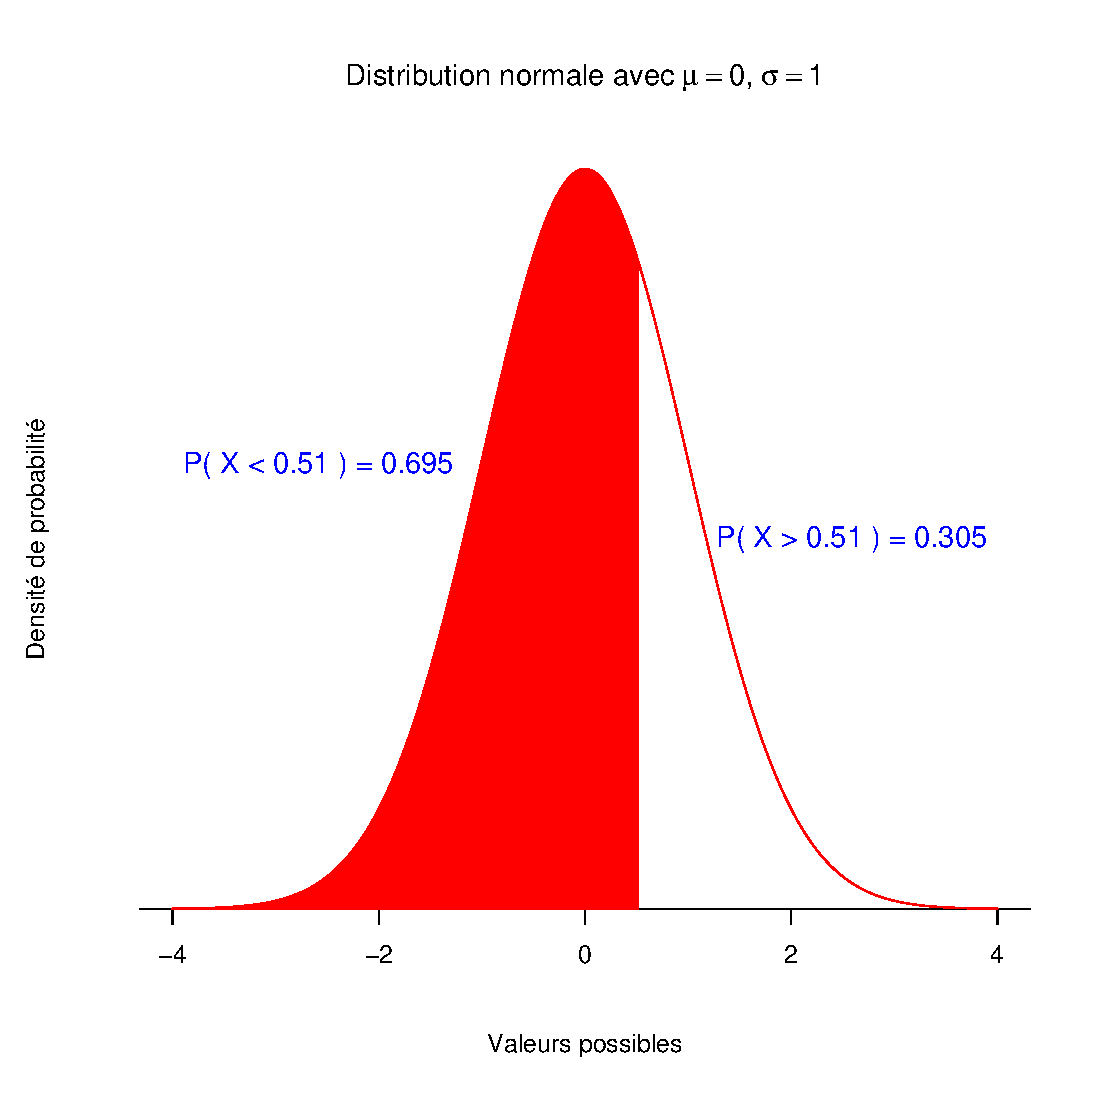
\includegraphics[scale=0.25]{norm_table}$$
%% Avec R
% x <- seq(0,3.09,by=0.01)
% z <- matrix(signif(pnorm(x),digits=4), ncol=10, byrow=TRUE, dimnames = list( seq(0,3,by=0.1), seq(0.00,0.09,by=0.01) ))
% library(Hmisc)
% latex(z, file="") # print to screen instead of write into file y.tex
{\footnotesize \begin{center}
\begin{tabular}{r|rrrrrrrrrr}

         z &       0.00 &       0.01 &       0.02 &       0.03 &       0.04 &       0.05 &       0.06 &       0.07 &       0.08 &       0.09 \\ \hline

           &            &            &            &            &            &            &            &            &            &            \\

         0 &     0.5000 &     0.5040 &     0.5080 &     0.5120 &     0.5160 &     0.5199 &     0.5239 &     0.5279 &     0.5319 &     0.5359 \\

       0.1 &     0.5398 &     0.5438 &     0.5478 &     0.5517 &     0.5557 &     0.5596 &     0.5636 &     0.5675 &     0.5714 &     0.5753 \\

       0.2 &     0.5793 &     0.5832 &     0.5871 &     0.5910 &     0.5948 &     0.5987 &     0.6026 &     0.6064 &     0.6103 &     0.6141 \\

       0.3 &     0.6179 &     0.6217 &     0.6255 &     0.6293 &     0.6331 &     0.6368 &     0.6406 &     0.6443 &     0.6480 &     0.6517 \\

       0.4 &     0.6554 &     0.6591 &     0.6628 &     0.6664 &     0.6700 &     0.6736 &     0.6772 &     0.6808 &     0.6844 &     0.6879 \\

           &            &            &            &            &            &            &            &            &            &            \\

       0.5 &     0.6915 &     0.6950 &     0.6985 &     0.7019 &     0.7054 &     0.7088 &     0.7123 &     0.7157 &     0.7190 &     0.7224 \\

       0.6 &     0.7257 &     0.7291 &     0.7324 &     0.7357 &     0.7389 &     0.7422 &     0.7454 &     0.7486 &     0.7517 &     0.7549 \\

       0.7 &     0.7580 &     0.7611 &     0.7642 &     0.7673 &     0.7704 &     0.7734 &     0.7764 &     0.7794 &     0.7823 &     0.7852 \\

       0.8 &     0.7881 &     0.7910 &     0.7939 &     0.7967 &     0.7995 &     0.8023 &     0.8051 &     0.8078 &     0.8106 &     0.8133 \\

       0.9 &     0.8159 &     0.8186 &     0.8212 &     0.8238 &     0.8264 &     0.8289 &     0.8315 &     0.8340 &     0.8365 &     0.8389 \\

           &            &            &            &            &            &            &            &            &            &            \\

         1 &     0.8413 &     0.8438 &     0.8461 &     0.8485 &     0.8508 &     0.8531 &     0.8554 &     0.8577 &     0.8599 &     0.8621 \\

       1.1 &     0.8643 &     0.8665 &     0.8686 &     0.8708 &     0.8729 &     0.8749 &     0.8770 &     0.8790 &     0.8810 &     0.8830 \\

       1.2 &     0.8849 &     0.8869 &     0.8888 &     0.8907 &     0.8925 &     0.8944 &     0.8962 &     0.8980 &     0.8997 &     0.9015 \\

       1.3 &     0.9032 &     0.9049 &     0.9066 &     0.9082 &     0.9099 &     0.9115 &     0.9131 &     0.9147 &     0.9162 &     0.9177 \\

       1.4 &     0.9192 &     0.9207 &     0.9222 &     0.9236 &     0.9251 &     0.9265 &     0.9279 &     0.9292 &     0.9306 &     0.9319 \\

           &            &            &            &            &            &            &            &            &            &            \\

       1.5 &     0.9332 &     0.9345 &     0.9357 &     0.9370 &     0.9382 &     0.9394 &     0.9406 &     0.9418 &     0.9429 &     0.9441 \\

       1.6 &     0.9452 &     0.9463 &     0.9474 &     0.9484 &     0.9495 &     0.9505 &     0.9515 &     0.9525 &     0.9535 &     0.9545 \\

       1.7 &     0.9554 &     0.9564 &     0.9573 &     0.9582 &     0.9591 &     0.9599 &     0.9608 &     0.9616 &     0.9625 &     0.9633 \\

       1.8 &     0.9641 &     0.9649 &     0.9656 &     0.9664 &     0.9671 &     0.9678 &     0.9686 &     0.9693 &     0.9699 &     0.9706 \\

       1.9 &     0.9713 &     0.9719 &     0.9726 &     0.9732 &     0.9738 &     0.9744 &     0.9750 &     0.9756 &     0.9761 &     0.9767 \\

           &            &            &            &            &            &            &            &            &            &            \\

         2 &     0.9772 &     0.9778 &     0.9783 &     0.9788 &     0.9793 &     0.9798 &     0.9803 &     0.9808 &     0.9812 &     0.9817 \\

       2.1 &     0.9821 &     0.9826 &     0.9830 &     0.9834 &     0.9838 &     0.9842 &     0.9846 &     0.9850 &     0.9854 &     0.9857 \\

       2.2 &     0.9861 &     0.9864 &     0.9868 &     0.9871 &     0.9875 &     0.9878 &     0.9881 &     0.9884 &     0.9887 &     0.9890 \\

       2.3 &     0.9893 &     0.9896 &     0.9898 &     0.9901 &     0.9904 &     0.9906 &     0.9909 &     0.9911 &     0.9913 &     0.9916 \\

       2.4 &     0.9918 &     0.9920 &     0.9922 &     0.9925 &     0.9927 &     0.9929 &     0.9931 &     0.9932 &     0.9934 &     0.9936 \\

           &            &            &            &            &            &            &            &            &            &            \\

       2.5 &     0.9938 &     0.9940 &     0.9941 &     0.9943 &     0.9945 &     0.9946 &     0.9948 &     0.9949 &     0.9951 &     0.9952 \\

       2.6 &     0.9953 &     0.9955 &     0.9956 &     0.9957 &     0.9959 &     0.9960 &     0.9961 &     0.9962 &     0.9963 &     0.9964 \\

       2.7 &     0.9965 &     0.9966 &     0.9967 &     0.9968 &     0.9969 &     0.9970 &     0.9971 &     0.9972 &     0.9973 &     0.9974 \\

       2.8 &     0.9974 &     0.9975 &     0.9976 &     0.9977 &     0.9977 &     0.9978 &     0.9979 &     0.9979 &     0.9980 &     0.9981 \\

       2.9 &     0.9981 &     0.9982 &     0.9982 &     0.9983 &     0.9984 &     0.9984 &     0.9985 &     0.9985 &     0.9986 &     0.9986 \\

           &            &            &            &            &            &            &            &            &            &            \\

         3 &     0.9987 &     0.9987 &     0.9987 &     0.9988 &     0.9988 &     0.9989 &     0.9989 &     0.9989 &     0.9990 &     0.9990
\end{tabular} 
\end{center}}



\newpage
\section{Table de la loi du $\chi^2$}
\label{sec:tablechideux}
% \begin{center}
% \includegraphics[width=\linewidth,clip]{table_chi2}
% \end{center}
%
%% Avec R
% # Se mettre dans le bon r�pertoire
% setwd("C:/Documents and Settings/Varone/Mes documents/Cours/Stat_III/polycopie")
% # Degr�s de libert�
% dl <- c( seq(1,30,by=1),seq(40,100,by=10) )
% # Erreurs de premi�re esp�ce
% alpha <- c(0.995,0.99,0.975,0.95,0.9,0.1,0.05,0.025,0.01,0.005)
% # Fonction � utiliser pour trouver la valeur du pertile
% f <- function(dl,alpha ) round(qchisq(alpha,dl,lower.tail=FALSE),digits=4) 
% # Tableau des r�sultats
% q2 <- outer(dl,alpha,f)
% # Ent�te des lignes et colonnes du tableau de r�sultat
% dimnames(q2) <- list(dl,alpha)
% # Package pour convertir en LaTeX
% library(Hmisc)
% # Conversion en LaTeX
% latex(q2, file="tableChiCarre.tex") # print to screen instead of write into file y.tex
{\footnotesize % latex.default(q2, file = "tableq2.tex") 
%
 \begin{center}
 \begin{tabular}{l|rrrrrrrrrr}\hline
& \multicolumn{10}{c}{\bf Valeurs de $\alpha$}\\
&
\multicolumn{1}{c}{\bf 0.995}&
\multicolumn{1}{c}{\bf 0.99}&
\multicolumn{1}{c}{\bf 0.975}&
\multicolumn{1}{c}{\bf 0.95}&
\multicolumn{1}{c}{\bf 0.9}&
\multicolumn{1}{c}{\bf 0.1}&
\multicolumn{1}{c}{\bf 0.05}&
\multicolumn{1}{c}{\bf 0.025}&
\multicolumn{1}{c}{\bf 0.01}&
\multicolumn{1}{c}{\bf 0.005}\\
\hline
{\bf dl}\\
1&$ 0.0000$&$ 0.0002$&$ 0.0010$&$ 0.0039$&$ 0.0158$&$  2.7055$&$  3.8415$&$  5.0239$&$  6.6349$&$  7.8794$\\
2&$ 0.0100$&$ 0.0201$&$ 0.0506$&$ 0.1026$&$ 0.2107$&$  4.6052$&$  5.9915$&$  7.3778$&$  9.2103$&$ 10.5966$\\
3&$ 0.0717$&$ 0.1148$&$ 0.2158$&$ 0.3518$&$ 0.5844$&$  6.2514$&$  7.8147$&$  9.3484$&$ 11.3449$&$ 12.8382$\\
4&$ 0.2070$&$ 0.2971$&$ 0.4844$&$ 0.7107$&$ 1.0636$&$  7.7794$&$  9.4877$&$ 11.1433$&$ 13.2767$&$ 14.8603$\\
5&$ 0.4117$&$ 0.5543$&$ 0.8312$&$ 1.1455$&$ 1.6103$&$  9.2364$&$ 11.0705$&$ 12.8325$&$ 15.0863$&$ 16.7496$\\
6&$ 0.6757$&$ 0.8721$&$ 1.2373$&$ 1.6354$&$ 2.2041$&$ 10.6446$&$ 12.5916$&$ 14.4494$&$ 16.8119$&$ 18.5476$\\
7&$ 0.9893$&$ 1.2390$&$ 1.6899$&$ 2.1673$&$ 2.8331$&$ 12.0170$&$ 14.0671$&$ 16.0128$&$ 18.4753$&$ 20.2777$\\
8&$ 1.3444$&$ 1.6465$&$ 2.1797$&$ 2.7326$&$ 3.4895$&$ 13.3616$&$ 15.5073$&$ 17.5345$&$ 20.0902$&$ 21.9550$\\
9&$ 1.7349$&$ 2.0879$&$ 2.7004$&$ 3.3251$&$ 4.1682$&$ 14.6837$&$ 16.9190$&$ 19.0228$&$ 21.6660$&$ 23.5894$\\
10&$ 2.1559$&$ 2.5582$&$ 3.2470$&$ 3.9403$&$ 4.8652$&$ 15.9872$&$ 18.3070$&$ 20.4832$&$ 23.2093$&$ 25.1882$\\
11&$ 2.6032$&$ 3.0535$&$ 3.8157$&$ 4.5748$&$ 5.5778$&$ 17.2750$&$ 19.6751$&$ 21.9200$&$ 24.7250$&$ 26.7568$\\
12&$ 3.0738$&$ 3.5706$&$ 4.4038$&$ 5.2260$&$ 6.3038$&$ 18.5493$&$ 21.0261$&$ 23.3367$&$ 26.2170$&$ 28.2995$\\
13&$ 3.5650$&$ 4.1069$&$ 5.0088$&$ 5.8919$&$ 7.0415$&$ 19.8119$&$ 22.3620$&$ 24.7356$&$ 27.6882$&$ 29.8195$\\
14&$ 4.0747$&$ 4.6604$&$ 5.6287$&$ 6.5706$&$ 7.7895$&$ 21.0641$&$ 23.6848$&$ 26.1189$&$ 29.1412$&$ 31.3193$\\
15&$ 4.6009$&$ 5.2293$&$ 6.2621$&$ 7.2609$&$ 8.5468$&$ 22.3071$&$ 24.9958$&$ 27.4884$&$ 30.5779$&$ 32.8013$\\
16&$ 5.1422$&$ 5.8122$&$ 6.9077$&$ 7.9616$&$ 9.3122$&$ 23.5418$&$ 26.2962$&$ 28.8454$&$ 31.9999$&$ 34.2672$\\
17&$ 5.6972$&$ 6.4078$&$ 7.5642$&$ 8.6718$&$10.0852$&$ 24.7690$&$ 27.5871$&$ 30.1910$&$ 33.4087$&$ 35.7185$\\
18&$ 6.2648$&$ 7.0149$&$ 8.2307$&$ 9.3905$&$10.8649$&$ 25.9894$&$ 28.8693$&$ 31.5264$&$ 34.8053$&$ 37.1565$\\
19&$ 6.8440$&$ 7.6327$&$ 8.9065$&$10.1170$&$11.6509$&$ 27.2036$&$ 30.1435$&$ 32.8523$&$ 36.1909$&$ 38.5823$\\
20&$ 7.4338$&$ 8.2604$&$ 9.5908$&$10.8508$&$12.4426$&$ 28.4120$&$ 31.4104$&$ 34.1696$&$ 37.5662$&$ 39.9968$\\
21&$ 8.0337$&$ 8.8972$&$10.2829$&$11.5913$&$13.2396$&$ 29.6151$&$ 32.6706$&$ 35.4789$&$ 38.9322$&$ 41.4011$\\
22&$ 8.6427$&$ 9.5425$&$10.9823$&$12.3380$&$14.0415$&$ 30.8133$&$ 33.9244$&$ 36.7807$&$ 40.2894$&$ 42.7957$\\
23&$ 9.2604$&$10.1957$&$11.6886$&$13.0905$&$14.8480$&$ 32.0069$&$ 35.1725$&$ 38.0756$&$ 41.6384$&$ 44.1813$\\
24&$ 9.8862$&$10.8564$&$12.4012$&$13.8484$&$15.6587$&$ 33.1962$&$ 36.4150$&$ 39.3641$&$ 42.9798$&$ 45.5585$\\
25&$10.5197$&$11.5240$&$13.1197$&$14.6114$&$16.4734$&$ 34.3816$&$ 37.6525$&$ 40.6465$&$ 44.3141$&$ 46.9279$\\
26&$11.1602$&$12.1981$&$13.8439$&$15.3792$&$17.2919$&$ 35.5632$&$ 38.8851$&$ 41.9232$&$ 45.6417$&$ 48.2899$\\
27&$11.8076$&$12.8785$&$14.5734$&$16.1514$&$18.1139$&$ 36.7412$&$ 40.1133$&$ 43.1945$&$ 46.9629$&$ 49.6449$\\
28&$12.4613$&$13.5647$&$15.3079$&$16.9279$&$18.9392$&$ 37.9159$&$ 41.3371$&$ 44.4608$&$ 48.2782$&$ 50.9934$\\
29&$13.1211$&$14.2565$&$16.0471$&$17.7084$&$19.7677$&$ 39.0875$&$ 42.5570$&$ 45.7223$&$ 49.5879$&$ 52.3356$\\
30&$13.7867$&$14.9535$&$16.7908$&$18.4927$&$20.5992$&$ 40.2560$&$ 43.7730$&$ 46.9792$&$ 50.8922$&$ 53.6720$\\
40&$20.7065$&$22.1643$&$24.4330$&$26.5093$&$29.0505$&$ 51.8051$&$ 55.7585$&$ 59.3417$&$ 63.6907$&$ 66.7660$\\
50&$27.9907$&$29.7067$&$32.3574$&$34.7643$&$37.6886$&$ 63.1671$&$ 67.5048$&$ 71.4202$&$ 76.1539$&$ 79.4900$\\
60&$35.5345$&$37.4849$&$40.4817$&$43.1880$&$46.4589$&$ 74.3970$&$ 79.0819$&$ 83.2977$&$ 88.3794$&$ 91.9517$\\
70&$43.2752$&$45.4417$&$48.7576$&$51.7393$&$55.3289$&$ 85.5270$&$ 90.5312$&$ 95.0232$&$100.4252$&$104.2149$\\
80&$51.1719$&$53.5401$&$57.1532$&$60.3915$&$64.2778$&$ 96.5782$&$101.8795$&$106.6286$&$112.3288$&$116.3211$\\
90&$59.1963$&$61.7541$&$65.6466$&$69.1260$&$73.2911$&$107.5650$&$113.1453$&$118.1359$&$124.1163$&$128.2989$\\
100&$67.3276$&$70.0649$&$74.2219$&$77.9295$&$82.3581$&$118.4980$&$124.3421$&$129.5612$&$135.8067$&$140.1695$\\
\hline
\end{tabular}
\end{center}

}

\newpage
\section{Table de la loi de Student}
%\begin{center}
%\includegraphics[width=\linewidth,clip]{table_student}
%\end{center}
%% Avec R
% # Se mettre dans le bon r�pertoire
% setwd("C:/Documents and Settings/Varone/Mes documents/Cours/Stat_III/polycopie")
% # Degr�s de libert�
% dl <- c( seq(1,30,by=1),seq(40,100,by=10),200,500)
% # Erreurs de premi�re esp�ce
% alphaonetail <- c(0.45,0.4,0.3,0.25,0.2,0.1,0.05,0.025,0.01,0.005)
% # Fonction � utiliser pour trouver la valeur du pertile
% f <- function(dl,alphaonetail ) round(qt(alphaonetail,dl, lower.tail=FALSE),digits=4) 
% # Tableau des r�sultats
% t <- outer(dl,alphaonetail,f)
% # Ent�te des lignes et colonnes du tableau de r�sultat
% dimnames(t) <- list(dl,alphaonetail)
% # Package pour convertir en LaTeX
% library(Hmisc)
% # Conversion en LaTeX
% latex(t, file="tableStudent.tex") # print to screen instead of write into file y.tex
{\footnotesize % latex.default(t, file = "tableStudent.tex") 
%
\begin{center}
 \begin{tabular}{r|rrrrrrrrrr}
$t$ & \multicolumn{10}{c}{\bf Valeurs de $\alpha$}\\
&
\multicolumn{1}{c}{\bf 0.45}&
\multicolumn{1}{c}{\bf 0.4}&
\multicolumn{1}{c}{\bf 0.3}&
\multicolumn{1}{c}{\bf 0.25}&
\multicolumn{1}{c}{\bf 0.2}&
\multicolumn{1}{c}{\bf 0.1}&
\multicolumn{1}{c}{\bf 0.05}&
\multicolumn{1}{c}{\bf 0.025}&
\multicolumn{1}{c}{\bf 0.01}&
\multicolumn{1}{c}{\bf 0.005}\\
\hline
{\bf dl} & \\
1&$0.1584$&$0.3249$&$0.7265$&$1.0000$&$1.3764$&$3.0777$&$6.3138$&$12.7062$&$31.8205$&$63.6567$\\
2&$0.1421$&$0.2887$&$0.6172$&$0.8165$&$1.0607$&$1.8856$&$2.9200$&$ 4.3027$&$ 6.9646$&$ 9.9248$\\
3&$0.1366$&$0.2767$&$0.5844$&$0.7649$&$0.9785$&$1.6377$&$2.3534$&$ 3.1824$&$ 4.5407$&$ 5.8409$\\
4&$0.1338$&$0.2707$&$0.5686$&$0.7407$&$0.9410$&$1.5332$&$2.1318$&$ 2.7764$&$ 3.7469$&$ 4.6041$\\
5&$0.1322$&$0.2672$&$0.5594$&$0.7267$&$0.9195$&$1.4759$&$2.0150$&$ 2.5706$&$ 3.3649$&$ 4.0321$\\
6&$0.1311$&$0.2648$&$0.5534$&$0.7176$&$0.9057$&$1.4398$&$1.9432$&$ 2.4469$&$ 3.1427$&$ 3.7074$\\
7&$0.1303$&$0.2632$&$0.5491$&$0.7111$&$0.8960$&$1.4149$&$1.8946$&$ 2.3646$&$ 2.9980$&$ 3.4995$\\
8&$0.1297$&$0.2619$&$0.5459$&$0.7064$&$0.8889$&$1.3968$&$1.8595$&$ 2.3060$&$ 2.8965$&$ 3.3554$\\
9&$0.1293$&$0.2610$&$0.5435$&$0.7027$&$0.8834$&$1.3830$&$1.8331$&$ 2.2622$&$ 2.8214$&$ 3.2498$\\
10&$0.1289$&$0.2602$&$0.5415$&$0.6998$&$0.8791$&$1.3722$&$1.8125$&$ 2.2281$&$ 2.7638$&$ 3.1693$\\
11&$0.1286$&$0.2596$&$0.5399$&$0.6974$&$0.8755$&$1.3634$&$1.7959$&$ 2.2010$&$ 2.7181$&$ 3.1058$\\
12&$0.1283$&$0.2590$&$0.5386$&$0.6955$&$0.8726$&$1.3562$&$1.7823$&$ 2.1788$&$ 2.6810$&$ 3.0545$\\
13&$0.1281$&$0.2586$&$0.5375$&$0.6938$&$0.8702$&$1.3502$&$1.7709$&$ 2.1604$&$ 2.6503$&$ 3.0123$\\
14&$0.1280$&$0.2582$&$0.5366$&$0.6924$&$0.8681$&$1.3450$&$1.7613$&$ 2.1448$&$ 2.6245$&$ 2.9768$\\
15&$0.1278$&$0.2579$&$0.5357$&$0.6912$&$0.8662$&$1.3406$&$1.7531$&$ 2.1314$&$ 2.6025$&$ 2.9467$\\
16&$0.1277$&$0.2576$&$0.5350$&$0.6901$&$0.8647$&$1.3368$&$1.7459$&$ 2.1199$&$ 2.5835$&$ 2.9208$\\
17&$0.1276$&$0.2573$&$0.5344$&$0.6892$&$0.8633$&$1.3334$&$1.7396$&$ 2.1098$&$ 2.5669$&$ 2.8982$\\
18&$0.1274$&$0.2571$&$0.5338$&$0.6884$&$0.8620$&$1.3304$&$1.7341$&$ 2.1009$&$ 2.5524$&$ 2.8784$\\
19&$0.1274$&$0.2569$&$0.5333$&$0.6876$&$0.8610$&$1.3277$&$1.7291$&$ 2.0930$&$ 2.5395$&$ 2.8609$\\
20&$0.1273$&$0.2567$&$0.5329$&$0.6870$&$0.8600$&$1.3253$&$1.7247$&$ 2.0860$&$ 2.5280$&$ 2.8453$\\
21&$0.1272$&$0.2566$&$0.5325$&$0.6864$&$0.8591$&$1.3232$&$1.7207$&$ 2.0796$&$ 2.5176$&$ 2.8314$\\
22&$0.1271$&$0.2564$&$0.5321$&$0.6858$&$0.8583$&$1.3212$&$1.7171$&$ 2.0739$&$ 2.5083$&$ 2.8188$\\
23&$0.1271$&$0.2563$&$0.5317$&$0.6853$&$0.8575$&$1.3195$&$1.7139$&$ 2.0687$&$ 2.4999$&$ 2.8073$\\
24&$0.1270$&$0.2562$&$0.5314$&$0.6848$&$0.8569$&$1.3178$&$1.7109$&$ 2.0639$&$ 2.4922$&$ 2.7969$\\
25&$0.1269$&$0.2561$&$0.5312$&$0.6844$&$0.8562$&$1.3163$&$1.7081$&$ 2.0595$&$ 2.4851$&$ 2.7874$\\
26&$0.1269$&$0.2560$&$0.5309$&$0.6840$&$0.8557$&$1.3150$&$1.7056$&$ 2.0555$&$ 2.4786$&$ 2.7787$\\
27&$0.1268$&$0.2559$&$0.5306$&$0.6837$&$0.8551$&$1.3137$&$1.7033$&$ 2.0518$&$ 2.4727$&$ 2.7707$\\
28&$0.1268$&$0.2558$&$0.5304$&$0.6834$&$0.8546$&$1.3125$&$1.7011$&$ 2.0484$&$ 2.4671$&$ 2.7633$\\
29&$0.1268$&$0.2557$&$0.5302$&$0.6830$&$0.8542$&$1.3114$&$1.6991$&$ 2.0452$&$ 2.4620$&$ 2.7564$\\
30&$0.1267$&$0.2556$&$0.5300$&$0.6828$&$0.8538$&$1.3104$&$1.6973$&$ 2.0423$&$ 2.4573$&$ 2.7500$\\
40&$0.1265$&$0.2550$&$0.5286$&$0.6807$&$0.8507$&$1.3031$&$1.6839$&$ 2.0211$&$ 2.4233$&$ 2.7045$\\
50&$0.1263$&$0.2547$&$0.5278$&$0.6794$&$0.8489$&$1.2987$&$1.6759$&$ 2.0086$&$ 2.4033$&$ 2.6778$\\
60&$0.1262$&$0.2545$&$0.5272$&$0.6786$&$0.8477$&$1.2958$&$1.6706$&$ 2.0003$&$ 2.3901$&$ 2.6603$\\
70&$0.1261$&$0.2543$&$0.5268$&$0.6780$&$0.8468$&$1.2938$&$1.6669$&$ 1.9944$&$ 2.3808$&$ 2.6479$\\
80&$0.1261$&$0.2542$&$0.5265$&$0.6776$&$0.8461$&$1.2922$&$1.6641$&$ 1.9901$&$ 2.3739$&$ 2.6387$\\
90&$0.1260$&$0.2541$&$0.5263$&$0.6772$&$0.8456$&$1.2910$&$1.6620$&$ 1.9867$&$ 2.3685$&$ 2.6316$\\
100&$0.1260$&$0.2540$&$0.5261$&$0.6770$&$0.8452$&$1.2901$&$1.6602$&$ 1.9840$&$ 2.3642$&$ 2.6259$\\
200&$0.1258$&$0.2537$&$0.5252$&$0.6757$&$0.8434$&$1.2858$&$1.6525$&$ 1.9719$&$ 2.3451$&$ 2.6006$\\
500&$0.1257$&$0.2535$&$0.5247$&$0.6750$&$0.8423$&$1.2832$&$1.6479$&$ 1.9647$&$ 2.3338$&$ 2.5857$\\
$\infty$ & \multicolumn{10}{c}{cf. Distribution Normale}
\end{tabular}

\end{center}

}

% \newpage
% \section{Table de la loi de Fisher, $p$=0.95}
% \begin{center}
% \includegraphics[width=\linewidth,clip]{table_fisher_95}
% \end{center}
%
% \newpage
% \section{Table de la loi de Fisher, $p$=0.99}
% \begin{center}
% \includegraphics[width=\linewidth,clip]{table_fisher_99}
% \end{center}


%\newpage
%\section{Table du test des rangs sign�s de Wilcoxon}\label{sec:wilcoxonsigne}
%Les valeurs critiques sont donn�es par la table suivante:\\[5mm]
%%
\begin{center}
 \begin{tabular}{r|rrr}
  unilat�ral & $\alpha = 0.05$ & $\alpha = 0.025$ & $\alpha = 0.01$\\
   bilat�ral & $\alpha = 0.10$ & $\alpha = 0.05$ & $\alpha = 0.02$\\
  \hline\\
  $n$ & \multicolumn{3}{c}{Inf�rieur, Sup�rieur}\\
  \hline
  5 &  0,15 & & \\
  6 &  2,19 &  0,21 & \\
  7 &  3,25 &  2,26 &  0,28\\
  8 &  5,31 &  3,33 &  1,35\\
  9 &  8,37 &  5,40 &  3,42\\
 10 & 10,45 &  8,47 &  5,50\\
 11 & 13,53 & 10,56 &  7,59\\
 12 & 17,61 & 13,65 & 10,68\\
 13 & 21,70 & 17,74 & 12,79\\
 14 & 25,80 & 21,84 & 16,89\\
 15 & 30,90 & 25,95 & 19,101\\
 16 & 35,101 & 29,107 & 23,113\\
 17 & 41,112 & 34,119 & 27,126\\
 18 & 47,124 & 40,131 & 32,139\\
 19 & 53,137 & 46,144 & 37,153\\
 20 & 60,150 & 52,158 & 43,167
\end{tabular}
\end{center}

% \newpage
% \section{Table du test de la somme des rangs de Wilcoxon}
%$$\includegraphics[width=\linewidth,clip]{table_wilcoxon}$$



\chapter{Instructions pour logiciels}

Voici quelques instructions pour quelques logiciels disponibles sur les ordinateurs de la HEG Gen\`eve.

\section{Loi normale}
\begin{tabular}{lc|l@{ = }l}
	Logiciel & Version \\
	\hline
	Calc d'OpenOffice & 2.4 & $z_{\alpha}$ & {\sc loi.normale.standard.inverse}()\\
	 &  & $p$ & {\sc loi.normale}()\\
	MS Excel & 2010 & $z_{\alpha}$ & {\sc loi.normale.inverse.n}()\\
	 &  & $p$ & {\sc loi.normale.n}()\\
	R & 2.13 & $z_{\alpha}$ & qnorm()\\
	  &       & $p$          & pnorm()\\
\end{tabular}

\begin{ex}
Calculer les valeurs critiques $z_{\alpha/2}$ pour un degr\'e de confiance $1-\alpha=0.9$ dans un test bilat\'eral, i.e. tels que $P(z_{\alpha/2})=0.9$

\begin{tabular}{|rl|}
\hline
	R & qnorm(0.1/2) ; qnorm(1-0.1/2)\\
	Ms Excel & {\sc =loi.normale.standard.inverse.n(0.1/2)}\\
	Calc & = {\sc loi.normale.standard.inverse(0.1/2)}\\
\hline
\end{tabular}
\end{ex}

\section{$t$-distribution}
\begin{tabular}{lc|l@{ = }l}
	Logiciel & Version \\
	\hline
	Calc d'OpenOffice & 2.4 & $t_{\alpha}$ & {\sc loi.student.inverse}()\\
	 &  & $p$ & {\sc loi.student}()\\
	MS Excel & 2010 & $t_{\alpha}$ & {\sc loi.student.inverse.n}()\\
	 &  & $p$ & {\sc loi.student.n}()\\
	R & 2.13 & $t_{\alpha}$ & qt()\\
	  &       & $p$          & pt()\\
\end{tabular}

\begin{ex}
Calculer les valeurs critiques pour un degr\'e de confiance $1-\alpha=0.95$ dans un test unilat\'eral avec 10 degr\'es de libert\'e.

\begin{tabular}{|rl|}
\hline
	R & qt(0.95, 10)\\
	Ms Excel & {\sc =loi.student.inverse.n(0.95;10)}\\
	Calc & {\sc =loi.student.inverse(2*0.05;10)}\\
\hline
\end{tabular}
\end{ex}


\section{$\chi^2_n$ distribution}
\begin{tabular}{lc|l@{ = }l}
	Logiciel & Version\\
	\hline
	Calc d'OpenOffice & 2.4 & $\ki^2_{1-\alpha}$ & {\sc khideux.inverse}()\\
	 &  & $p$ & 1-{\sc loi.khideux}()\\
	MS Excel & 2010 & $\ki^2_{1-\alpha}$ & {\sc loi.khideux.inverse}()\\
	 &  & $p$ & 1-{\sc loi.khideux.n}()\\
	R & 2.13 & $\ki^2_{\alpha}$ & {\sc qchisq}()\\
	  &       & $p$          & pchisq()\\
\end{tabular}

\begin{ex}
Calculer la valeur critique pour un degr\'e de confiance $1-\alpha=0.9$ dans un test unilat\'eral avec 19 degr\'es de libert\'e.

\begin{tabular}{|rl|}
\hline
	R & qchisq(0.9,19)\\
	Ms Excel & {\sc =loi.khideux.inverse.(0.9;19)}\\
	Calc & {\sc =khideux.inverse(0.1;19)}\\
\hline
\end{tabular}
\end{ex}

\section{Intervalle de confiance}
La fonction {\sc intervalle.confiance} d'Excel et Calc d'OpenOffice ne calculent pas un intervalle de confiance, mais la marge d'erreur dans le cas suivant: la population suit une loi normale, et son \'ecart type est connu.

\begin{tabular}{lc|l}
	Logiciel & Version \\
	\hline
	Calc d'OpenOffice & 2.4 & $\mbox{Marge}_z$ = {\sc intervalle.confiance}()\\
	MS Excel & 2010 & $\mbox{Marge}_z$ = {\sc intervalle.confiance}()\\
	R & 2.13 & $IC_t$ = t.test()\$conf.int\\
\\
\end{tabular}

\begin{ex}
Calculer la marge de l'IC pour une moyenne, dont l'\'ecart type connu de la population est 0.04, le degr\'e de confiance vaut 0.95, la taille de l'\'echantillon est 4 et la population suit une loi normale.\\[5mm]
\begin{tabular}{|rl|}
\hline
	Ms Excel & {\sc =intervalle.confiance(0.05;0.04;4)}\\
	Calc & {\sc =intervalle.confiance(0.05;0.04;4)}\\
\hline
\end{tabular}

\vspace{5mm}
Reprenons l'exemple en \ref{exICMoyenneStudent}\\[5mm]
\begin{tabular}{|rl|}
\hline
	R:  x <- & c(7.1,13.6,1.4,3.6,1.9,11.6,1.7,16.9,2.6,7.7,\\
	         & 12.4,11,3.7,14.6,8.8,8.5,6.1,3.3,6.1,6.9,0.4,11,0.8,6.4,9.1)
\\
 & t.test(x)\$conf.int\\
\hline
\end{tabular}
\end{ex}

\section{Test d'une moyenne}
\begin{tabular}{lc|l}
	Logiciel & Version \\
	\hline
	Ms Excel & 2010 & {\sc =test.student}()\\
	R & 2.13 & t.test\\
	 & & library(TeachingDemos); z.test()\\
\\
\end{tabular}

\begin{ex}
Test unilat\'eral de la moyenne:  $H_0: \mu\leq 5.2$ lorsque la variance est inconnue, pour un \'echantillon de taille 15, et un seuil de signification de 0.05.

\begin{tabular}{|rl|}
\hline
	Ms Excel & {\sc =test.student(x,5.2;1;3)}\\
	R:  & x <- c(4,4.1,6,5.5,5.8,4.2,3.1,6,4.9,3.9,4.8,5.6,5.7,5.3,5.8)\\
	    & t.test(x, mu = 5.2, alternative = "greater", correct=FALSE)\\
\hline
\end{tabular}
\end{ex}

\begin{ex}
Test bilat\'eral de la moyenne:  $H_0: \mu= 99$ lorsque l'\'ecart type est connu ($\sigma = 5$) , avec un seuil de signification de 0.05.

\begin{tabular}{|rl|}
\hline
	R:  & x <- rnorm(25, 100, 5)\\
	    & library(TeachingDemos); z.test(x, mu = 99, stdev= 5)\\
\hline
\end{tabular}
\end{ex}

\section{Test d'une proportion}
\begin{tabular}{lc|l}
	Logiciel & Version \\
	\hline
	R & 2.9.1 & prop.test\\
\\
\end{tabular}

\begin{ex}
Reprenons l'exemple \ref{exTestProportion}, dans lequel 9 contrats sur 600 \'etaient incomplets. La banque exige qu'il n'y ait pas plus d'1\% de contrats incomplets, avec un niveau de signification fix\'e \`a 0.02. 

\begin{tabular}{|rl|}
\hline
	R:  & prop.test(9, 600, p=0.01, alternative="greater", conf.level = 0.98, correct=FALSE)\\
\hline
\end{tabular}
\end{ex}

\section{Test d'une variance}
 
\begin{ex}
Tester si la variance est est en dessous de 0.005.\\
Valeurs: -0.04,  0.11, -0.10,  0.05,  0.20, -0.05, -0.04,  0.13,  0.01,  0.05, -0.05,  0.04, -0.03,  0.11,  0.05, -0.03, -0.21,  0.19,  0.04, -0.14\\
H0: $\sigma^2\leq 0.005$\\
H1: $\sigma^2> 0.005$

\begin{verbatim}
y <- c( -0.04,  0.11, -0.10,  0.05,  0.20, -0.05, -0.04,  0.13,  0.01,  0.05,-0.05,  0.04, -0.03,  0.11,  0.05, -0.03, -0.21,  0.19,  0.04, -0.14)
sigmacarre = 0.005
p= pchisq( var(y)*(length(y)-1)/sigmacarre, length(y)-1,lower.tail=FALSE)
\end{verbatim}
\end{ex}

%\section{Test des rangs sign\'es de Wilcoxon}
%\begin{tabular}{lc|l@{ = }l}
%	Logiciel & Version \\
%	\hline
%	R & 2.9.1 &  & wilcox.test()
%\end{tabular}
%
%\begin{ex}
%Tester si la valeur de la m\'ediane est de 40.
%
%\begin{verbatim}
%x <- c(31, 48, 23, 56, 28, 29, 44)
%wilcox.test(x, alternative = "two.sided", mu=40, 
%            exact = TRUE, conf.level=0.9, conf.int = TRUE)
%\end{verbatim}
%\end{ex}

\section{Test d'ind\'ependance}
\begin{tabular}{lc|l@{ = }l}
	Logiciel & Version \\
	\hline
	R & 2.9.1 &  & chisq.test()
\end{tabular}

\begin{ex}
D\'eterminer si deux variables sont ind\'ependantes.

\begin{verbatim}
amendes <- matrix(c(240,160,80,40,32,18,11,9,5,4),ncol=5,byrow=TRUE)
rownames(amendes)<-c("Homme","Femme")
colnames(amendes)<-c("Vitesse","Parcage","Feux grillés","Service_AP", "Autre")
amendes <- as.table(amendes)
chisq.test(amendes)
\end{verbatim}
\end{ex}

\section{Test de corr\'elation lin\'eaire}
\begin{tabular}{lc|l@{ = }l}
	Logiciel & Version \\
	\hline
	R & 2.9.1 &  & cor.test()
\end{tabular}

\begin{ex}
D\'eterminer si deux variables sont positivement corr\'el\'ees (lin\'eairement).

\begin{verbatim}
taille <- c(90, 160, 250, 160, 200, 160, 200, 200, 160, 90)
proportion <- c(0.13, 0.16, 0.21, 0.18, 0.18, 0.19, 0.15, 0.17, 0.13, 0.11)
cor.test(taille, proportion, method = "pearson", alternative = "greater")
\end{verbatim}
\end{ex}

\section{R\'egression lin\'eaire}
\begin{tabular}{lc|l@{ = }l}
	Logiciel & Version \\
	\hline
	R & 2.9.1 &  & lm()
\end{tabular}

\begin{ex}
\begin{verbatim}
x <- c(3,5,2,8,2,6,7,1,4,2,9,6)
y <- c(487,445,272,641,187,440,346,238,312,269,655,563)
lm(y~x) # coefficients
summary(lm.D90 <- lm(y ~ x)) # avec tests
\end{verbatim}
\end{ex}

%  \chapter{Exercices}
 

 %%%%%%%%%%%%%%%%%%%%%%%%%%%%%%%%%%%%%%%%%%%%%%%%%%%%%%%%%%%%%%%%%%%%%%%%%%%%%
 %%%%%%%%%%%%%%%%%%%%%%%%%%%%%%%%%%%%%%%%%%%%%%%%%%%%%%%%%%%%%%%%%%%%%%%%%%%%%
 %%%%%%%%%%%%%%%%%%%%%%%%%%%%%%%%%%%%%%%%%%%%%%%%%%%%%%%%%%%%%%%%%%%%%%%%%%%%%
 %%%%%%%%%%%%%%%%%%%%%%%%%%%%%%%%%%%%%%%%%%%%%%%%%%%%%%%%%%%%%%%%%%%%%%%%%%%%%
 \section{Introduction}

 \subsection{}

 Nous nous int�ressons aux succursales des diff�rentes cha�nes de la grande distribution alimentaire en Suisse. Nous disposons de donn�es
r�colt�es aupr�s de 8 succursales genevoises de la Migros.

 \begin{enumerate}
    \item Les 8 succursales pour lesquelles nous disposons de donn�es constituent-elles une population ou un �chantillon?
    \item Peut-on dire que chacune des 8 succursales consid�r�e est une unit� statistique?
    \item Quelle est la population qui nous int�resse?
    \item Dans quelles conditions pourrait-on dire que les 8 succursales consid�r�es sont une population?
 \end{enumerate}

 %%%%%%%%%%%%%%%%%%%%%%%%%%%%%%%%%%%%%%%%%%%%%%%%%%%%%%%%%%%%%%%%%%%%%%%%%%%%%
 %%%%%%%%%%%%%%%%%%%%%%%%%%%%%%%%%%%%%%%%%%%%%%%%%%%%%%%%%%%%%%%%%%%%%%%%%%%%%
 %%%%%%%%%%%%%%%%%%%%%%%%%%%%%%%%%%%%%%%%%%%%%%%%%%%%%%%%%%%%%%%%%%%%%%%%%%%%%
 %%%%%%%%%%%%%%%%%%%%%%%%%%%%%%%%%%%%%%%%%%%%%%%%%%%%%%%%%%%%%%%%%%%%%%%%%%%%%

 \section{Lois de probabilit� continues}

 \subsection{}

 Soit une variable $Z$ distribu�e selon une loi normale centr�e-r�duite. Calculer la probabilit� pour la variable $Z$ de se trouver
dans chacun des cas suivants:

 \begin{enumerate}
    \item Entre $z=0$ et $z=1.2$.
    \item Entre $z=-0.68$ et $z=0$.
    \item Entre $z=-0.46$ et $z=2.21$.
    \item Entre $z=0.81$ et $z=1.94$.
    \item A gauche de $z=-0.6$.
    \item A droite de $z=-1.28$.
    \item A droite de $z=2.05$ et � gauche de $z=-1.44$.
    \item A droite de $z=2.05$ ou � gauche de $z=-1.44$.
 \end{enumerate}


 \subsection{}

 Soit $Z$, une variable al�atoire suivant une loi
normale centr�e et  r�duite $N(0,1)$.

 \begin{enumerate}
 \item % 1
D�terminer la probabilit� des �v�nements suivants :
 \begin{enumerate}
    \item $Z < 2.14$
    \item $Z < -2.14$
    \item $Z \in [-2.14 \; ;\; 2.14]$
 \end{enumerate}
 \item % 2
 Pour quel seuil $a$ a-t-on $P(Z < a) = p$ lorsque $p$ prend les
valeurs  suivantes : 
 \begin{enumerate}
    \item $p = 0.8686$
    \item $p = 0.9719$
    \item $p = 0.2912$
 \end{enumerate}

 \hspace*{-6ex} Soit $X$, une variable al�atoire suivant une loi normale $N(2,1)$.

 \item % 3
 D�terminer les probabilit�s suivantes :
 \begin{enumerate}
    \item $P(X < 3.98)$
    \item $P(X < 1.5)$
    \item $P(X \in  [2\;;\;3])$
 \end{enumerate}

 \item % 4
 Pour quelle valeur de $a$ a-t-on :
 \begin{enumerate}
    \item $P(X < a) = 0.7454$
    \item $P(-a+2 < X < a+2) = 0.7458$
 \end{enumerate}

 \hspace*{-6ex} Soit $Y$, une variable al�atoire suivant une loi normale $N(2,9)$.

 \item % 5
 D�terminer les probabilit�s suivantes:
 \begin{enumerate}
    \item $P(Y < 4.25)$
    \item $P(Y < 1.5)$
    \item $P( |Y| < 1)$
 \end{enumerate}

 \item % 6
   Pour quelle valeur de $a$ a-t-on: 
   \begin{enumerate}
    \item $P(Y < a) = 0.64$
    \item $P(a < Y < 2.5) = 0.3788$
    \item $P(- a < Y < a) = 0.9$
 \end{enumerate}
 \end{enumerate}



 \subsection{}

 Un ensemble de scores d'arithm�tique obtenus par des enfants de quatri�me ann�e pr�sente
une moyenne de 30 et un �cart type de 6. Un ensemble de scores obtenus par des enfants de
neuvi�me ann�e pr�sente une moyenne de 36 et un �cart type de 12. Nous supposons que les
distributions sont normales.
 
 \begin{enumerate}
    \item Faites un sch�ma approximatif de ces donn�es en
repr�sentant les deux groupes sur la m�me figure.
    \item Quel pourcentage des �l�ves de quatri�me ann�e
obtiennent-ils de meilleurs scores que la moyenne des �l�ves de
neuvi�me ann�e?
    \item Quel pourcentage des �l�ves de neuvi�me ann�e
obtiennent-ils de moins bons scores que la moyenne des �l�ves de
quatri�me ann�e?
 \end{enumerate}




 \subsection{}

 \begin{enumerate}
 \item % 1
 Soit la variable $X$ suivant une loi normale $N(10,4)$.\\ Calculer
$P(8 <X<13).$
 \item % 2
 Soit la variable $Q_{10}$ suivant une loi du chi-2 � 10 degr�s de libert�.
 \newline
 D�terminer $P(Q_{10} < 12.55),$ $P(Q_{10} > 18.31),$ $P(Q_{10} <
18.31)$ et $P(12.55 < Q_{10} < 18.31)$.
 \newline
 Trouver la valeur $a$ telle que $P(Q_{10} < a) = 0.975$.
 \item % 3
 Soit la variable $T_{8}$ suivant une loi de Student � 8 degr�s de
libert�.
 \newline
 D�terminer $P(T_{8} < 0.546)$,
 $P(T_{8} < - 0.546),$ $ P( - 0.546 < T_{8} < 1.86)$.
 \newline
 Trouver la valeur $b$ telle que $P(T_{8}> b) = 0.6$.
 \item % 4
 Soit la variable $F_{8,5}$ suivant une loi de Fisher-Snedecor 
� 8 et 5 degr�s de libert�.
 \newline
 Trouver la valeur de $c$ telle que $P (F_{8,5} < c) = 0.95$.
 \item % 5
 Soit la variable $F_{5,8}$ suivant une loi de Fisher-Snedecor � 5
et 8 degr�s de libert�.
 \newline
 Trouver la valeur $d$ telle que $P(F_{5,8} < d) = 0.95$.
 \item % 6
 Soit la variable $F_{12,3}$ suivant une loi de Fisher-Snedecor
� 12 et 3 degr�s de libert�.
 \newline
 Trouver la valeur de $e$ telle que $P (F_{12,3} < e) = 0.99$.
 \item % 7
 Soit la variable $F_{3,12}$ suivant une loi de Fisher-Snedecor � 3
et 12 degr�s de libert�.
 \newline
 Trouver la valeur $f$ telle que $P(F_{3,12} < f) = 0.99$.
 \end{enumerate}


 \subsection{}

 Les lois Binomiale, de Poisson, Normale et du Chi-2 sont 4 des lois de distribution statistique les plus utilis�es. Pour chacune des 4
situations d�crites ci-dessous, choisissez la loi la plus adapt�e. Attention: vous devez choisir une et une seule fois chacune des 4 lois
propos�es.\\

 \begin{enumerate}
    \item Nous voulons effectuer un test portant sur le rapport entre deux variances.

    \item Nous �tudions la distribution du nombre mensuel de faillites dans le canton de Gen�ve.

    \item Nous nous int�ressons au nombre de femmes pr�sentes dans un �chantillon de 25 personnes travaillant dans le domaine du
graphisme.

    \item Nous �tudions la distribution du r�sultat net apr�s imp�ts en 2005 des soci�t�s suisses fond�es en 2005.

 \end{enumerate}        



 %%%%%%%%%%%%%%%%%%%%%%%%%%%%%%%%%%%%%%%%%%%%%%%%%%%%%%%%%%%%%%%%%%%%%%%%%%%%%
 %%%%%%%%%%%%%%%%%%%%%%%%%%%%%%%%%%%%%%%%%%%%%%%%%%%%%%%%%%%%%%%%%%%%%%%%%%%%%
 %%%%%%%%%%%%%%%%%%%%%%%%%%%%%%%%%%%%%%%%%%%%%%%%%%%%%%%%%%%%%%%%%%%%%%%%%%%%%
 %%%%%%%%%%%%%%%%%%%%%%%%%%%%%%%%%%%%%%%%%%%%%%%%%%%%%%%%%%%%%%%%%%%%%%%%%%%%%
 \section{Estimation}

 \subsection{}

 Soit $Y$ le nombre de personnes qui assistent � la repr�sentation
d'une pi�ce de th��tre.
 \begin{enumerate}
 \item Pour 5 jours de repr�sentation pris au hasard on a observ�:
 $$
 \begin{array}{l|ccccc}
 i & 1 & 2 & 3 & 4 & 5\\
 \hline
 y_i & 300 & 280 & 290 & 310 & 295
 \end{array}
 $$
 Estimer l'esp�rance $\E(Y) = \mu $ par la m�diane de l'�chantillon
$\dot Y$, puis par la moyenne de l'�chantillon $\overline{Y}$.

 \item Pour 4 nouveaux jours choisis au hasard on a observ� :
 $$
 \begin{array}{l|cccc}
 i & 6 & 7 & 8 & 9\\
 \hline
 y_i & 305 & 318 & 290 & 280
 \end{array}
 $$
 Recalculer les deux estimations de $\mu $ en consid�rant
l'�chantillon form� par l'ensemble des 9 observations. Commenter.

 \item Pour les cinq premi�res observations on trouve:
 $$
 \sum\limits^5_{i=1} y^2_i = 435'625
 $$
 et pour l'ensemble des 9 observations:
 $$
 \sum\limits^9_{i=1} y^2_i = 792'274
 $$
 Donner une estimation non-biais�e de la variance de $Y$, ainsi qu'une estimation
non-biais�e de l'�cart type de $\overline{Y}$ dans chacun des deux cas consid�r�s.
Commenter.

 \item Supposons maintenant qu'� la suite d'une erreur le nombre
d'entr�es du 9�me jour ait �t� mal relev�. De ce fait nous avons:
 $$
 \begin{array}{l|ccccccccc}
 i & 1 & 2 & 3 & 4 & 5 & 6 & 7 & 8 & 9\\
 \hline
 y_i & 300 & 280 & 290 & 310 & 295 & 305 & 318 & 290 & 28
 \end{array}
 $$
 Recalculer les deux estimations de $\mu $. Lequel des deux estimateurs est-il le plus
pertinent?
 \end{enumerate}



 \subsection{}

 Dans une soci�t� de services ayant r�cemment engag� de nombreux nouveaux employ�s, deux �chantillons ont �t� pr�lev�s, l'un parmi
l'ancien personnel et l'autre parmi le nouveau. On a demand� au hasard � 10 anciens employ�s et � 6 nouveaux d'�valuer sur une
�chelle allant de 0 � 20 l'efficacit� de l'organisation interne de l'entreprise. Les r�sultats suivants ont �t� obtenus:

 \bigskip
 \begin{center}
 \begin{tabular}{lcccccccccc}
 anciens employ�s & 12 & 4 & 5 & 13 & 9 & 7 & 6 & 12 & 11 & 16\\
 \hline
 nouveaux employ�s & 5 & 3 & 4 & 2 & 12 & 7\\
 \end{tabular}
 \end{center}

 Les moyennes respectives des deux �chantillons sont 10.2 et 5.5, et les intervalles de confiance correspondants calcul�s avec un
risque $\alpha$=5\% valent $[7.3 ; 13.1]$ et $[1.7 ; 9.3]$. Commentez ces donn�es et d�terminez si les populations d'anciens et
nouveaux employ�s ont ou non une opinion similaire quant � l'efficacit� de l'organisation interne de l'entreprise.



 \subsection{}

 Les responsables canadiens et fran�ais du d�partement vente d'une soci�t� produisant des super-ordinateurs d�sirent comparer leurs
r�sultats mensuels respectifs. Pour ce faire, ils disposent d'informations sur la distribution des variables $C$: ventes mensuelles
au Canada durant les 24 derniers mois d'exploitation et $F$: ventes mensuelles en France durant les 24 derniers mois d'exploitation:

 \vspace{2ex}
 Intervalle de confiance ($\alpha$=5\%) pour la moyenne: C: $[12 ; 20]$, F: $[4 ; 16]$.\\
 Intervalle de confiance ($\alpha$=5\%) pour la variance: C: $[2 ; 11]$, F: $[12 ; 28]$.\\
 Intervalle de confiance ($\alpha$=5\%) pour le coefficient de corr�lation lin�aire: $[0.54 ; 0.98]$.

 \vspace{2ex}
 A l'aide de ces informations, comparez les variables $C$ et $F$.




 \subsection{}

 Dans le but d'estimer le nombre moyen de passagers (conducteur
compris) par v�hicule automobile circulant sur l'autoroute
Gen�ve-Lausanne, un observateur a recueilli les donn�es suivantes:

 \begin{center}
 \begin{tabular}{lccccccr}
 \hline\hline
 Nombre de passagers & 1 & 2 & 3 & 4 & 5 & 6 & Total\\
 Effectif & 230 & 248 & 117 & 76 & 14 & 3 & 688\\
 \hline
 \end{tabular}
 \end{center}

 Estimer la moyenne $\mu$ et la variance $\sigma^2$ de la population � l'aide d'intervalles de confiance � 95\%.






 %%%%%%%%%%%%%%%%%%%%%%%%%%%%%%%%%%%%%%%%%%%%%%%%%%%%%%%%%%%%%%%%%%%%%%%%%%%%%
 %%%%%%%%%%%%%%%%%%%%%%%%%%%%%%%%%%%%%%%%%%%%%%%%%%%%%%%%%%%%%%%%%%%%%%%%%%%%%
 %%%%%%%%%%%%%%%%%%%%%%%%%%%%%%%%%%%%%%%%%%%%%%%%%%%%%%%%%%%%%%%%%%%%%%%%%%%%%
 %%%%%%%%%%%%%%%%%%%%%%%%%%%%%%%%%%%%%%%%%%%%%%%%%%%%%%%%%%%%%%%%%%%%%%%%%%%%%
 \section{Tests d'hypoth�ses}

 \subsection{}

 Afin de d�terminer si le taux de participation des Suisses aux votations est en augmentation, le test suivant a �t� r�alis� sur la
base d'un �chantillon repr�sentatif de donn�es:

 \vspace{2ex}
 $H_0$: le taux de participation est constant sur les 3 derni�res ann�es\\
 $H_1$: le taux de participation a significativement augment� au cours des 3 derni�res ann�es

 \vspace{2ex}
 La $p$-valeur du test vaut 0.03. Conclure en prenant un risque de premi�re esp�ce �gale � 5\%.



 \subsection{}

 En 2002 et 2003, sur la base de deux �chantillons de taille 20, une soci�t� d'assurances a sign� chaque jour en moyenne
respectivement 115 et 108 nouveaux contrats. Un test unilat�ral � gauche ($\alpha$=5\%) dont l'hypoth�se nulle �tait: ``les nombres
moyens de nouveaux contrats sign�s par jour sont identiques en 2002 et 2003'' a conduit � une $p$-valeur de 0.45. Selon vous, peut-on
d�s lors raisonnablement admettre que cette soci�t� a sign� journellement le m�me nombre de contrats en 2002 et 2003?



 \subsection{}

 Les donn�es suivantes repr�sentent le taux d'acceptation d'une
initiative pour un �chantillon de communes en Suisse.

 $$
 \begin{array}{cccccc}
 62.3 & 44.4 & 49.2 & 63.3 & 47.6 & 60.1 \\
 37.4 & 55.8 & 57.5 & 58.3 & 56.2 & 54.3
 \end{array}
 $$

  \noindent On suppose que l'�cart type des taux pour l'ensemble
des communes suisses vaut 5.

 \begin{enumerate}
 \item En prenant un risque de premi�re esp�ce $\alpha = 0.05$, la moyenne $\mu$ des
taux de la population de communes est-elle significativement sup�rieure � 50\%?
Commenter. Formellement, on testera:

 $$
 \begin{array}{ll}
 & H_0 : \mu = \mu_0 = 50 \\
 \mbox{ contre} & H_1 : \mu = \mu_1 > 50
 \end{array}
 $$

 \item Soit un �chantillon de taille 100 pour lequel on a obtenu la m�me
moyenne que pour l'�chantillon pr�c�dent de taille 12. D�terminer la r�gion
critique du test pour ce nouvel �chantillon et comparer avec celle obtenue au point 1.
Commenter.
 \end{enumerate}




 \subsection{}

 En 2005, une enqu�te men�e aupr�s de femmes quant � leur �ge $x_i$ � la naissance de leur premier enfant a donn�, pour 51 femmes
interrog�es au hasard, les r�sultats suivants: $$ \bar{x} = 28 \mbox{ ann�es } $$ $$ n s^2 = \sum (x_i - \bar{x})^2 = 816 \:
\mbox{ann�es}^2  $$ Les �ges $x_i$ repr�sentent les r�alisations d'une variable al�atoire $X$ distribu�e selon une loi normale ($\mu$,
$\sigma^2$).
 
  \begin{enumerate} 
 
  \item On sait qu'en 1990, pour la population, l'�ge moyen des femmes � la naissance de
leur premier enfant �tait de 27 ans. Peut-on affirmer, avec un degr� de confiance de 95
\%,  que l'�ge moyen a augment� en 3 ans ? Pour cela, on testera l'hypoth�se $H_0$ :
$\mu=27$ contre l'hypoth�se $H_1$ : $\mu>27$ .
 
  \item Selon certains chercheurs, l'�cart type $s$ de l'�chantillon sous-estime l'�cart
type $\sigma $ de la population, qu'ils �valuent � 5 ans. Refaire le test pr�c�dent en
supposant que la vraie valeur de $\sigma $ est �gale � 5 et commenter.
 
  \item Tester l'hypoth�se $H_0 : \sigma = \sigma_0 = 5$ contre l'hypoth�se $H_1 :
\sigma = \sigma_1 < \sigma_0$ avec un risque de premi�re esp�ce de 5\%. Commenter.
 
  \end{enumerate}



 \subsection{}

 Dans une grande entreprise am�ricaine, le salaire annuel moyen des
hommes poss�dant entre 3 et 5 ans d'exp�rience est de 58'000\$. Les salaires (en milliers de dollars) d'un �chantillon al�atoire de 10
femmes poss�dant entre 3 et 5 ans d'exp�rience sont les suivants:
 \[
    54 \quad 57 \quad 61 \quad 51 \quad 49 \quad 56 \quad 60 \quad 52 \quad 45 \quad 66
 \]
 Y a-t-il des preuves attestant de niveaux de salaires diff�rents
pour les hommes et les femmes?



 \subsection{}

 Supposons que
 \begin{itemize}
    \item $X$ suive une distribution normale d'esp�rance 100 et
d'�cart type 20 sous $H_0$;
    \item $X$ suive une distribution normale d'esp�rance 80 et
d'�cart type 20 sous $H_1$.
 \end{itemize}

 Nous optons pour un test unilat�ral � gauche.
 \begin{enumerate}
    \item En choisissant une erreur de premi�re esp�ce
$\alpha=5\%$, que vaut le seuil de rejet $r$?
    \item En choisissant une erreur de premi�re esp�ce
$\alpha=1\%$, que vaut le seuil de rejet $r$?
    \item Calculer la probabilit� de commettre une erreur de
seconde esp�ce en fixant la probabilit� de l'erreur de premi�re
esp�ce � $\alpha=5\%$.
    \item Calculer la probabilit� de commettre une erreur de
seconde esp�ce en fixant la probabilit� de l'erreur de premi�re
esp�ce � $\alpha=1\%$.
 \end{enumerate}




 %%%%%%%%%%%%%%%%%%%%%%%%%%%%%%%%%%%%%%%%%%%%%%%%%%%%%%%%%%%%%%%%%%%%%%%%%%%%%
 %%%%%%%%%%%%%%%%%%%%%%%%%%%%%%%%%%%%%%%%%%%%%%%%%%%%%%%%%%%%%%%%%%%%%%%%%%%%%
 %%%%%%%%%%%%%%%%%%%%%%%%%%%%%%%%%%%%%%%%%%%%%%%%%%%%%%%%%%%%%%%%%%%%%%%%%%%%%
 %%%%%%%%%%%%%%%%%%%%%%%%%%%%%%%%%%%%%%%%%%%%%%%%%%%%%%%%%%%%%%%%%%%%%%%%%%%%%
 \section{Comparaisons param�triques}

 \subsection{}

 Une firme agro-alimentaire lance sur le march� le nouveau yoghourt ``Borc''. Apr�s quelques mois, elle doit
se rendre � l'�vidence~: les ventes sont m�diocres. Le service marketing sugg�re de changer le nom en ``Miam''. Quelque temps plus tard,
la firme veut savoir si cette modification a port� ses fruits. Elle dispose des donn�es suivantes sur les ventes, en milliers d'unit�s
pour une semaine, relev�es dans divers hypermarch�s de taille comparable~:

 \begin{center} \begin{tabular}{|c|cc|} \hline Ventes de~: &
``Borc'' ($X$) & ``Miam'' ($Y$) \\ \hline & 7 & 8.5 \\ & 5.6 & 5.6 \\ & 3.2 & 6 \\ & 4.2 & 4.9 \\ \hline Moyennes & 5 & 6.25 \\ Variances
& 2.04 & 1.8425 \\ \hline \end{tabular} \end{center}

 \begin{enumerate}

 \item On suppose que les ventes proviennent d'hypermarch�s tir�s
au hasard � chaque p�riode. Tester (avec un risque de premi�re
esp�ce de 10\%) si le changement de nom a amen� une hausse
significative des ventes.

 \item Effectuer le m�me test en consid�rant que les donn�es sont
appari�es.

 \end{enumerate}





 \subsection{}

   Le tableau suivant donne les taux de syndicalisation en
pourcents d'entreprises choisies au hasard dans l'industrie d'une
part et les services d'autre part: 

 $$ \begin{array}{lccccc}
 \mbox{ Industrie } & 50 & 60 & 60 & 50 &\\
 \mbox{ Services } & 30 & 30 & 50 & 80 & 55
 \end{array}
 $$

 \begin{enumerate}
 \item D�terminer si la variance des taux de syndicalisation est
identique dans les populations ``Industrie'' et ``Services''.
 \item Tester la diff�rence des moyennes en utilisant un test de
Student appropri�.
 \end{enumerate}



 \subsection{}

 Nous voulons comparer les effets de deux anesth�siques $X$ et $Y$ qui procurent
respectivement des dur�es de sommeil al�atoires de moyennes $\mu_X$ et $\mu_Y$. Notre
hypoth�se dit que $X$ et $Y$ sont �galement efficace. Pour v�rifier cette hypoth�se,
nous allons effectuer un test bilat�ral comparant les moyennes, en supposant que les
variances des populations sont in�gales. Nous disposons de 11 observations ind�pendantes,
6 pour l'�chantillon $X$ et 5 pour $Y$:

 \begin{center}
 \begin{tabular}{ccccccc}
 \hline\hline
 $X$ & 8.00 & 8.97 & 8.32 & 8.07 & 7.86 & 8.37\\
 $Y$ & 9.36 & 8.47 & 9.04 & 8.10 & 8.71 &\\
 \hline
 \end{tabular}
 \end{center}

 Conclure pour un degr� de confiance de 95\%.



 \subsection{}

 Un analyste au service du personnel d'une soci�t� de distribution
se demande quels sont les traits de personnalit� qui font qu'un
vendeur est un bon vendeur. En particulier, il veut savoir si le
fait d'�tre extraverti est un atout. Il choisit alors 20 vendeurs
connus comme excellents et 32 vendeurs m�diocres, et il leur fait
passer � tous un test d'extraversion. Les scores obtenus sont les
suivants, les valeurs les plus hautes marquant l'extraversion la
plus �lev�e:

 \vspace{1ex}
 \textit{Bons vendeurs:} 12, 17, 20, 19, 11, 9, 7, 4, 12, 15, 13,
18, 20, 16, 15, 16, 18, 13, 11, 10.

 \vspace{1ex}
 \textit{Vendeurs m�diocres:} 12, 7, 9, 13, 15, 17, 12, 11, 13, 10,
9, 8, 7, 15, 13, 6, 5, 5, 13, 15, 17, 19, 18, 20, 19, 17, 13, 16,
8, 6, 7, 8.

 \vspace{1ex}
 Utilisez le listing suivant, produit par SPSS, pour tester l'hypoth�se selon laquelle l'extraversion n'influence pas la performance des
vendeurs ($\alpha=5\%$).

  \begin{center}
   \includegraphics[width=\linewidth,clip]{ex_vendeurs}
  \end{center}









 %%%%%%%%%%%%%%%%%%%%%%%%%%%%%%%%%%%%%%%%%%%%%%%%%%%%%%%%%%%%%%%%%%%%%%%%%%%%%
 %%%%%%%%%%%%%%%%%%%%%%%%%%%%%%%%%%%%%%%%%%%%%%%%%%%%%%%%%%%%%%%%%%%%%%%%%%%%%
 %%%%%%%%%%%%%%%%%%%%%%%%%%%%%%%%%%%%%%%%%%%%%%%%%%%%%%%%%%%%%%%%%%%%%%%%%%%%%
 %%%%%%%%%%%%%%%%%%%%%%%%%%%%%%%%%%%%%%%%%%%%%%%%%%%%%%%%%%%%%%%%%%%%%%%%%%%%%
 \section{Comparaisons non-param�triques}

 \subsection{}

 Dans une institution, on a pr�lev� deux �chantillons : l'un
parmi  l'ancien personnel et l'autre parmi le nouveau. On a demand� au
hasard  � 10 anciens employ�s et � 6 nouveaux d'�valuer sur une �chelle
allant  de 0 � 20 l'efficacit� de la nouvelle organisation interne.

 \bigskip
 \noindent On a obtenu les r�sultats suivants:

 \bigskip
 \begin{center}
 \begin{tabular}{ll}
 anciens & 12; \ 4; \ 5; \ 13; \ 9; \ 14;\ 6;\ 12;\ 11;\ 16\\
 employ�s & \\
 \hline
 nouveaux & 5;\ 3;\ 4;\ 2;\ 12;\ 7\\
 employ�s &\\
 \end{tabular}
 \end{center}

 \begin{enumerate}
 \item Au vu des donn�es ci-dessus, peut-on admettre que les
opinions des  nouveaux et des anciens employ�s se distribuent de
fa�on analogue?
 \item Effectuer un test bilat�ral de la somme des rangs de Wilcoxon
avec un risque $\alpha $ de 5\%. Commenter.
 \end{enumerate}


 \subsection{}

 On examine l'�ge d'entr�e dans l'enseignement primaire pour
diff�rents pays. On consid�re un �chantillon de pays asiatiques et
un �chantillon de pays europ�ens et on arrive aux �ges suivants:

 \begin{center} \begin{tabular}{|c|cccccc|} \hline Asie & 4 & 6 & 5
& & & \\ \hline Europe & 4 & 5 & 6 & 6 & 7 & 7 \\ \hline
\end{tabular} \end{center}

 Tester, en utilisant la statistique de la somme des rangs de
Wilcoxon, si les �ges d'entr�e diff�rent significativement entre les
deux continents (on prendra $\alpha=5\%$).



 \subsection{}

   Voici des �chantillons des salaires horaires de base pratiqu�s par des entreprises de  deux branches industrielles:

 \begin{center} \begin{tabular}{|c|c|} \hline &\\ B�timent & Automobile\\ &\\ \hline &\\ 15 & 12\\ 12 & 16\\ 16 & 16\\
   & 16\\
 \hline
 \end{tabular}
 \end{center}


 Effectuer le test de Wilcoxon. Peut-on admettre une diff�rence significative � $5\%$ entre les salaires horaires des deux branches?







 \subsection{}
						 
 On a observ� le d�ficit budg�taire de 10 villes europ�ennes en 2004, 2005, et 2006 (les villes observ�es restant les m�mes). En faisant
la diff�rence ``d�ficit de 2005'' moins ``d�ficit de 2004'' on a constat� que 9 villes avaient une diff�rence positive et 1 une diff�rence
n�gative. En faisant la diff�rence ``d�ficit de 2006'' moins ``d�ficit de 2005'' on a constat� que 7 villes avaient une diff�rence
positive et 3 une diff�rence n�gative.\\

 Effectuer deux tests du signe bilat�raux avec un risque $\alpha=5\%$, le premier entre 2004 et 2005 et le second entre 2005 et 2006.
Commenter.



\end{document}

%%% Local Variables:
%%% mode: latex

%%% TeX-master: t
%%% End:
